 \documentclass[12pt,spanish]{article}
    %preámbulo
\textheight = 21cm
\textwidth = 16cm
\topmargin = -1cm
\oddsidemargin= 0.5cm
\parindent = 0mm

\usepackage{mathtools}
\usepackage[utf8]{inputenc}
\usepackage{graphicx}
\usepackage{subfig}
\usepackage{colortbl}
\usepackage{enumitem}
\usepackage[hidelinks,breaklinks=true]{hyperref}
\usepackage[nottoc]{tocbibind}
\usepackage[table,xcdraw]{xcolor}

\setlist{nolistsep}
\usepackage{graphicx}
\hypersetup{
    colorlinks   = true,
    allcolors    = blue,
    linktoc=all,     %set to all if you want both sections and subsections linked
    linkcolor=black,  %choose some color if you want links to stand out
}
\renewcommand{\familydefault}{\sfdefault}

%COLOR
\usepackage{color}
\definecolor{gray97}{gray}{.97}
\definecolor{gray75}{gray}{.75}
\definecolor{gray45}{gray}{.45}
\renewcommand{\baselinestretch}{1.5}
\renewcommand{\arraystretch}{.7}

%FLOWCHART
\usepackage[utf8]{inputenc}
\usepackage{tikz}
\usetikzlibrary{shapes.geometric, arrows}

\tikzstyle{startstop} = 
[rectangle, rounded corners, minimum width=3cm, minimum height=1cm,text centered, draw=black, fill=red!30]
\tikzstyle{io} = 
[trapezium, trapezium left angle=70, trapezium right angle=110, draw=black, fill=blue!30,text width=4.5cm]
\tikzstyle{process} = 
[rectangle,draw=black,fill=orange!30,text width=(\textwidth-2*\gap)/3,]
\tikzstyle{decision} = 
[diamond, text centered, draw=black, fill=green!30, aspect=2]
\tikzstyle{arrow} = [thick,->,>=stealth]

%DEFINIR CODIGO EN HTML
\usepackage{listings}
\lstset{literate=
  {á}{{\'a}}1 {é}{{\'e}}1 {í}{{\'i}}1 {ó}{{\'o}}1 {ú}{{\'u}}1
  {Á}{{\'A}}1 {É}{{\'E}}1 {Í}{{\'I}}1 {Ó}{{\'O}}1 {Ú}{{\'U}}1
  {à}{{\`a}}1 {è}{{\`e}}1 {ì}{{\`i}}1 {ò}{{\`o}}1 {ù}{{\`u}}1
  {À}{{\`A}}1 {È}{{\'E}}1 {Ì}{{\`I}}1 {Ò}{{\`O}}1 {Ù}{{\`U}}1
  {ä}{{\"a}}1 {ë}{{\"e}}1 {ï}{{\"i}}1 {ö}{{\"o}}1 {ü}{{\"u}}1
  {Ä}{{\"A}}1 {Ë}{{\"E}}1 {Ï}{{\"I}}1 {Ö}{{\"O}}1 {Ü}{{\"U}}1
  {â}{{\^a}}1 {ê}{{\^e}}1 {î}{{\^i}}1 {ô}{{\^o}}1 {û}{{\^u}}1
  {Â}{{\^A}}1 {Ê}{{\^E}}1 {Î}{{\^I}}1 {Ô}{{\^O}}1 {Û}{{\^U}}1
  {œ}{{\oe}}1 {Œ}{{\OE}}1 {æ}{{\ae}}1 {Æ}{{\AE}}1 {ß}{{\ss}}1
  {ç}{{\c c}}1 {Ç}{{\c C}}1 {ø}{{\o}}1 {å}{{\r a}}1 {Å}{{\r A}}1
  {€}{{\EUR}}1 {£}{{\pounds}}1
}
\lstset{ 
frame=Ltb,
framerule=0pt,
aboveskip=0.5cm,
framextopmargin=2pt,
framexbottommargin=2pt,
framexleftmargin=0.4cm,
framesep=0pt,
rulesep=.4pt,
backgroundcolor=\color{white},
rulesepcolor=\color{black},
%
stringstyle=\ttfamily,
showstringspaces = false,
basicstyle=\fontsize{9}{4}\ttfamily,
commentstyle=\color{gray45},
keywordstyle=\bfseries,
%
numbers=left,
numbersep=15pt,
numberstyle=\tiny,
numberfirstline = false,
breaklines=true,
lineskip=-1pt,
tabsize=1, 
}

\DeclareCaptionFormat{listing}{\rule{\dimexpr\textwidth+17pt\relax}{0.4pt}\par\vskip1pt#1#2#3}
\captionsetup[lstlisting]{format=listing,singlelinecheck=false, margin=0pt, font={sf},labelsep=space,labelfont=bf}

\lstnewenvironment{listing}[1][]{\lstset{#1}\pagebreak[0]}{\pagebreak[0]}
\lstdefinestyle{consola} 
{
basicstyle=\scriptsize\bf\ttfamily,
backgroundcolor=\color{gray75},
}
\lstdefinestyle{HTML}{language=HTML,}
\lstdefinestyle{JAVA}{language=JAVA,}


\usepackage{fancyhdr}
\pagestyle{fancy}
\fancyhf{}
\fancyhead[LE,RO]{ }
\fancyhead[RE,LO]{Instituto Tecnológico de Veracruz}
\fancyfoot[CE,CO]{\thepage}

\usepackage[fixlanguage]{babelbib}
\usepackage[english,spanish]{babel}
\bibliographystyle{babalpha}

\renewcommand{\headrule}{\hrule height 2pt \vspace{1mm}\hrule height 1pt}
\renewcommand{\footrulewidth}{1pt}

    
\begin{document}
    \renewcommand{\contentsname}{Índice}
    \renewcommand{\listfigurename}{Lista de figuras}
    \renewcommand{\listtablename}{Lista de tablas}
    \renewcommand\lstlistingname{Código}
    \renewcommand\lstlistlistingname {Lista de códigos}
    \renewcommand{\figurename}{Figura}
    \renewcommand{\tablename}{Tabla}
    \renewcommand{\refname}{Referencias bibliográficas}
    \numberwithin{figure}{section}
    \numberwithin{lstlisting}{section}
    \numberwithin{table}{section} 
    \begin{titlepage}
\thispagestyle{empty}

\newcommand{\titulo}[1]{\def\eltitulo{#1}}
\newcommand{\carrera}[1]{\def\lacarrera{#1}}
\newcommand{\nombre}[1]{\def\elnombre{#1}}    %* Del alumno
\newcommand{\director}[1]{\def\eldirector{#1}}  %* De tesis
\newcommand{\fecha}[1]{\def\lafecha{#1}}

%% Llena los siguientes datos (usa MAYÚSCULAS)
%%Estos datos aparecerán en la portada y los encabezados
\titulo{Una propuesta para resolver el problema del agente viajero basado en agrupamiento por cuadrantes y  su implementación usando metaheurísticas}
\nombre{{Guillermo Sebastián Medina Palacios}}
\carrera{Ingeniero en Sistemas Computacionales}
\director{{M.C. Rafael Rivera López}\\{Dr. Marco Antonio Cruz Chávez}}
\fecha{2017}

%% Barra izquierda - Escudos
%\hskip-1.5cm
\begin{minipage}[c][10cm][s]{3cm} 
  \begin{center}
  
   
\includegraphics[height=2.6cm]{Imagenes/LogoITV.jpg}\\[10pt]

    \hskip2pt
    \vrule width2pt height17cm \hskip1mm
    \vrule width1pt height17cm    
    \\[10pt]
    
  \end{center}
\end{minipage}\quad
%% Barra derecha - Tí­tulos
\begin{minipage}[c][9.5cm][s]{10cm}
  \begin{center}
    % Barra superior
    {\Large Secretaría de Educación Pública}
	{\Large Tecnológico Nacional de México}
    \vspace{.3cm}
    \hrule height 2pt
    \vspace{.1cm}
    \hrule height 1pt
    \vspace{.3cm}
    {\large Instituto Tecnológico de Veracruz}

    % Titulo del trabajo
    \vspace{3cm}

    {\Large \eltitulo}

    \vspace{3cm}

    % Tipo de trabajo
    \makebox[8cm][s]{\Huge T E S I S}\\[8pt]
     PARA OBTENER EL T\'ITULO DE:\\[3pt]
    \mbox{}\lacarrera\\[13pt]
    PRESENTA:\\[3pt]
    \elnombre

    \vspace{2cm}

    {\small Asesores:\\ \eldirector}

    \vspace{2cm}

    \lafecha
    
  \end{center}
\end{minipage}
\end{titlepage}

    \renewcommand{\thepage}{\roman{page}}
    \clearpage \newpage
        \cleardoublepage
        \phantomsection
        \addcontentsline{toc}{section}{Dedicatoria}
        \section*{Dedicatoria}

\textit
{
Este trabajo está dedicado principalmente a mis padres que siempre me han llevado por el camino correcto, apoyando y presionando para terminar tanto mi carrera como este documento. Siempre me han dicho que lo más importante es la educación ya que es lo único que te puede garantizar una vida digna.\\
\hspace*{1cm} No somos ricos, ni tampoco somos de escasos recursos; con su esfuerzo me compraron mi primera laptop con la cual pude hacer mis proyectos de programación y gracias a ella fue con la que empezó mi carrera profesional, también agradezco a mi hermano quien espero que pronto también se titule.\\
\hspace*{1cm} También agradezco al profesor Rafael Rivera López quien me asesoró en este proyecto que inicie desde el servicio social y sobre todo con la documentación del mismo.\\
\hspace*{1cm} Agradezco mucho a mi jefe directo Noe Mendoza Viveros quien me dio la oportunidad de pertenecer al equipo de desarrollo de GOMSA Logística desde que fui residente poniendo en práctica mis habilidades como programador y embarcarme en el mundo laboral.\\
\hspace*{1cm} Por último debido a cuestiones de tiempo no puedo incluir sus nombres, pero agradezco a todos mis demás compañeros, familiares y maestros que he conocido a lo largo de mi vida tanto como estudiante como persona que de alguna grande o pequeña forma influenciaron en mi vida.\\
\hspace*{1cm} No importa el tiempo que pase siempre seremos estudiantes, ya que nunca dejamos de aprender.\\\\
\begin{flushright}
De todo corazón.\\
Guillermo Sebastián Medina Palacios.
\end{flushright}
}

\newpage
 
    \clearpage \newpage
        \cleardoublepage
        \phantomsection
        \addcontentsline{toc}{section}{Resumen}
        \section*{Resumen}
%El tema de este trabajo es acerca de la aplicación de un algoritmo que sigue un mismo camino, seguido de otro que se dedica a la selección de valores aleatorios. La combinación de ambas tecnicas permite crear mejores resultados que las de sus predecesores, donde cada nuevo "espécimen" sea probado, replicado o desechado según sea el caso.\\
%\hspace*{1cm}El objetivo de un algoritmo de inteligencia artificial (IA) es obtener un resultado a través de una serie de tareas y patrones establecidos para reaccionar ante cualquier situación. Sin embargo, también es necesario que exista ese factor de 'suerte', donde la IA pueda ir más allá de los esperado tomando caminos al azar, pero sin ignorar su concepto de sentido común, tal como hacen los seres humanos al tomar decisiones.\\
\hspace*{1cm}Este trabajo de tesis describe el desarrollo de una técnica para encontrar una solución al problema del agente viajero, que es una referencia clásica en el área de la optimización combinatoria y se utiliza como un caso de prueba estándar para evaluar la efectividad de diversos métodos de optimización.\\
\hspace*{1cm}La técnica propuesta en este documento utiliza una agrupación de soluciones parciales de un problema en cuadrantes del espacio euclidiano con el fin de obtener una solución cercana al óptimo a través de una regla determinística.\\
\hspace*{1cm}La solución inicial encontrada a través de este método es refinada en una etapa subsecuente utilizando un conjunto de metaheurísticas. Los resultados obtenidos indican que el uso de esta estrategia permite encontrar soluciones cercanas al óptimo para el problema del agente viajero.\\
\hspace*{1cm}En \cite{[REF1]} se indica que el problema del agente viajero es posiblemente el más importante de los problemas de optimización combinatoria ya que fue uno de los primeros en ser clasificados como “duros” técnicamente hablando.\\
\hspace*{1cm} El texto está dividido en los siguientes capítulos:
\begin{itemize}
\item \textbf{Marco metodológico: }El marco metodológico es el inicio de cada investigación, es una breve introducción que plantea el documento: la descripción del problema, la hipótesis propuesta, los objetivos que pretende alcanzar, las justificaciones de realizarlo, así como los alcances y las limitaciones que tiene del trabajo. En este caso se explicará la problemática del TSP y que tipo de solución se usará para resolver dicho problema.
\item \textbf{Marco teórico: }Para una mejor comprensión del tema, en este capítulo se describen todos los temas que fueron usados para el desarrollo de esta tesis, desde la definición del problema del agente viajero, así como de conceptos como metaheurística, la teoría de autómatas, etc. La intención de este capítulo es informar al lector y que pueda comprender la solución implementada en los siguientes capítulos. La información obtenida para el desarrollo de este capítulo es respaldada por fuentes de diversas instituciones.
\item \textbf{Método de agrupamiento basado en cuadrantes: }Éste es el nombre que se le dio al algoritmo para resolver las instancias del problema del agente viajero y en este capítulo se explica la forma en que trabaja. Básicamente, este algoritmo usa técnicas de agrupamiento para dividir el problema en otros más pequeños con la intención de reducir la explosión combinatoria del problema.
\item \textbf{Documentación del software usado en las pruebas: }En este capítulo se presenta una descripción del programa que se implementó en esta tesis. Se explica de que elementos se compone la interfaz, como funciona y el papel que desempeñan las metaheurísticas. Al final de este capítulo se hace una demostración de cómo se utilizó este programa para el desarrollo de los experimentos descritos en el siguiente capítulo.
\item \textbf{Pruebas y análisis de resultados: }Por último se usará el programa descrito en el capítulo anterior para realizar experimentos sobre varias instancias del problema del agente viajero conocidos dentro del medio. Estos problemas fueron obtenidos en la página de la Universidad de Heidelberg (\cite{[TSPLIB]}). Una vez terminado los experimentos se construyeron gráficas y se compararon los resultados obtenidos con los reportados en la literatura. Adicionalmente se aplica el método propuesto en este trabajo para resolver un grupo de problemas conocidos como "Arte con TSP". Una vez finalizado los capítulos, se presentan las conclusiones de este trabajo, así como las referencias bibliográficas. 
\end{itemize}
\newpage     
    \tableofcontents  
    \clearpage \newpage
        \listoffigures
    \clearpage \newpage
        \listoftables
    \clearpage \newpage
        \lstlistoflistings
        \addcontentsline{toc}{section}{\lstlistlistingname}
  %\clearpage \newpage
        %\cleardoublepage
        %\phantomsection 
    \clearpage \newpage
        \renewcommand{\thepage}{\arabic{page}}
        \setcounter{page}{1}
        \chapter{}
    \vspace*{10cm}
    \begin{center}
        %\thispagestyle{empty} 
        \section*{ CAPÍTULO 1 : Marco metodológico }
        \addcontentsline{toc}{section}{CAPÍTULO 1 : Marco metodológico}
        \addtocounter{section}{1}
        \setcounter{subsection}{0} 
        \setcounter{figure}{0}
        \setcounter{lstlisting}{0}
        \setcounter{table}{0}
    \end{center}

    \clearpage \newpage
    \vspace*{8cm}
    \subsection{Antecedentes}
\phantomsection
El problema del agente viajero (TSP por sus siglas en inglés) fue formulado en 1930 y según la teoría de la complejidad es considerado como un problema NP-Completo que, en otras palabras, no puede ser resuelto por métodos convencionales. El TSP está aplicado principalmente para el trazo de rutas vehiculares óptimas, al buscar la distancia más corta de un punto a otro.\\
\hspace*{1cm}Existen distintos enfoques y fuentes de información para el estudio y resolución del TSP. La fuente de información usada para este trabajo será la TSPLIB que es una agrupación de problemas de prueba para TSP para comparar el rendimiento de dichos enfoques. El conjunto de problemas que componen la TSPLIB fueron encontradas en la página de la Universidad de Heidelberg (\cite{[TSPLIB]}).\\
\hspace*{1cm}Dentro de los enfoques conocidos se encuentra el uso de metaheurísticas, que han probado ser eficientes para resolver problemas computacionales complejos incluyendo el TSP.\\

\subsection{Planteamiento del problema}
El problema inicia bajo la siguiente premisa: “Un viajero quiere pasar por una cantidad específica de lugares recorriendo la menor distancia y en el menor tiempo y regresar al punto de origen pasando por cada ciudad una sola vez”.\\ 
\hspace*{1cm}Este problema, aunque fácil de plantear es difícil resolver, ya que la cantidad de rutas posibles crecen de manera exponencial. En las tablas \ref {table:Cap1_1_1} y \ref {table:Cap1_1_2} se tiene un ejemplo de las combinaciones que se obtienen en función del número de ciudades pero partiendo del mismo punto de origen.
    
    \begin{table}[hbtp]
        \centering
        \caption{Rutas posibles con 2 lugares.}       
        \begin{tabular}{| l | l |  }
            \hline
             \rowcolor[gray]{0.9} 1  &  2 \\ \hline
             A  & B \\ \hline
        \end{tabular}
        \label{table:Cap1_1_1}
    \end{table}

\hspace*{1cm}En el ejemplo de la tabla \ref {table:Cap1_1_1} las combinaciones que se pueden realizar si el viaje fuera de 2 puntos sería solo 1; ahora realizando el mismo ejemplo pero calculando el número de rutas de 5 lugares se puede observar en la tabla \ref {table:Cap1_1_2} como el número de rutas aumenta.
    
    \begin{table}[hbtp]
        \centering
        \caption{Ejemplo con 5 lugares.}       
        \begin{tabular}{ | l | l | l | l | 1 |  }
            \hline
            \rowcolor[gray]{0.9}
            1 & 2 & 3 & 4 & 5 \\ \hline
            A & B & C & D & E \\ \hline
            A & B & C & E & D \\ \hline
            A & B & D & C & E \\ \hline
            A & B & D & E & C \\ \hline
            A & B & E & B & C \\ \hline
            A & B & E & C & B \\ \hline
        \end{tabular}
        \hspace*{0.1cm}
        \begin{tabular}{ | l | l | l | l | 1 |  }
            \hline
            \rowcolor[gray]{0.9}
            1 & 2 & 3 & 4 & 5 \\ \hline
            A & C & B & D & E \\ \hline
            A & C & B & E & D \\ \hline
            A & C & D & B & E \\ \hline
            A & C & D & E & B \\ \hline
            A & C & E & B & D \\ \hline
            A & C & E & D & B \\ \hline
        \end{tabular}
        \hspace*{0.1cm}
        \begin{tabular}{ | l | l | l | l | 1 |  }
            \hline
            \rowcolor[gray]{0.9}
            1 & 2 & 3 & 4 & 5 \\ \hline
            A & C & B & D & E \\ \hline
            A & C & B & E & D \\ \hline
            A & C & D & B & E \\ \hline
            A & C & D & E & B \\ \hline
            A & C & E & B & D \\ \hline
            A & C & E & D & B \\ \hline
        \end{tabular}
        \hspace*{0.1cm}
        \begin{tabular}{ | l | l | l | l | 1 |  }
            \hline
            \rowcolor[gray]{0.9}
            1 & 2 & 3 & 4 & 5 \\ \hline
            A & E & B & C & D \\ \hline
            A & E & B & D & C \\ \hline
            A & E & C & B & D \\ \hline
            A & E & C & D & B \\ \hline
            A & E & D & B & C \\ \hline
            A & E & D & C & B \\ \hline
        \end{tabular}
        \label{table:Cap1_1_2}
    \end{table}
    
    
\hspace*{1cm}Como se acaba de ver en la tabla \ref {table:Cap1_1_2} se pueden observar 24 combinaciones posibles a tomar; esta cantidad aumenta de manera exponencial de acuerdo al número de entradas (lugares) que recibe, lo que significa que entre más lugares tenga el problema más tiempo se ocupa para encontrar la ruta más corta.\\
\hspace*{1cm}La resolución del TSP a llamado la atención de la comunidad científica desde su formulación inicial. De acuerdo a \cite{[REF2]} las aplicaciones del TSP van más allá del problema de planear una ruta ya que se utiliza en varias áreas de conocimiento que incluyen las matemáticas, las ciencias computacionales, la investigación de operaciones, la genética y otras disciplinas de la ingeniería.\\ 
\hspace*{1cm}De acuerdo a lo anterior existen propuestas para su resolución que abarcan el uso de diversos algoritmos extraídos tanto de la teoría de grafos como de la inteligencia artificial. Estos algoritmos utilizan heurísticas tanto determinísticas según \cite{[REF4]} como aquellas basadas en la aleatoriedad según \cite{[REF5]}.\\
\hspace*{1cm}TSP es considerado como un problema de optimización que busca dentro de un conjunto de soluciones candidatas (las posibles rutas de viaje) aquella que presente el mejor resultado (en caso del TSP costo menor) respecto a todas las demás. Existen propuestas que consisten en partir de una solución inicial aplicando reglas para mejorar dicha solución, ó aquellas que trabajan con un grupo se soluciones cuya información se vuelve a combinar para generar nuevas soluciones.\\
\hspace*{1cm}Un aspecto importante en los algoritmos para resolver problemas de optimización es definir la solución inicial, generalmente se utiliza una solución inicial completamente aleatoria o una simple secuencia ordenada de ciudades según \cite{[REF3]}.\\
\hspace*{1cm}Por lo anterior, es posible definir el siguiente planteamiento: ¿Es posible encontrar una solución inicial del problema del agente viajero utilizando una técnica de agrupamiento basada en cuadrantes que sea competitiva o esté cercana al óptimo?

\subsection{Objetivos}
El objetivo general es crear un algoritmo que servirá para obtener una solución inicial a instancias del TSP, que servirá como base para aplicar una serie de metaheurísticas que refinarán la solución con el fin de obtener soluciones cercanas al óptimo.\\
\subsubsection{Objetivos específicos}
  \begin{itemize} 
    \item Desarrollar un algoritmo que permita obtener una solución cercana a la óptima.
    \item Hacer uso de los resultados obtenidos por medio del algoritmo anterior aplicándolo con metaheurísticas.  
    \item Crear un programa que sea capaz de realizar los procedimientos anteriores, también que lea y guarde archivos en “.TSPLIB”, este tipo de formato son los utilizados para resolver problemas de TSP.
    \item Comparar lo que se obtuvo por medio del programa con su respectivo benchmark y anotar los resultados tanto el costo de cada problema como de la imagen de la ruta creada por medio del programa.
  \end{itemize}
  
\subsection{Justificación}
Aunque ya existen formas de resolver el problema del agente viajero, se aportará con una forma novedosa para encontrar una solución inicial al problema.\\
\hspace*{1cm}También se demostrará que se pueden obtener rutas con resultados cercanos al óptimo usando un algoritmo de agrupamiento combinado con metaheurísticas.\\
\hspace*{1cm}Por último el programa se creará con la finalidad para demostrar de manera gráfica el potencial de los procedimientos ejecutados y observar los cambios. No está de más mencionar que cualquier problema resuelto se puede guardar en un archivo para volverlos a cargar cuando se necesite.

\subsection{Hipótesis}
%Basado en los resultados obtenidos se comprobará que el uso del método de agrupación basado en cuadrantes sirve para obtener resultados cercanos a sus respectivos benchmarks en un corto lapso de tiempo. El uso de metaheurísticas servirá para mejorar el resultado obtenido.\\
El uso del método de agrupación basado en cuadrantes con la ayuda de metaheurísticas, obtiene resultados cercanos a los reportados en la literatura en un lapso corto de tiempo, para  un conjunto de benchmarks seleccionados de la librería TSPLIB.\\

\subsection {Alcances}   
      \begin{itemize} 
		  \item El uso del algoritmo basado en cuadrantes en conjunción con una serie de metaheurísticas proporcionará soluciones cercanas al óptimo para el TSP.
		  \item El uso del programa, al poder leer archivos en formato .tsp permite que cualquier otro investigador del campo de TSP pueda utilizarlo para sus respectivas pruebas, un ejemplo están en los problemas encontrados en la página de la universidad de Waterloo según cite{[MONALISA]}, esto se describirá más a detalle en el tema \ref{subsection:ARTTSP}.
      \end{itemize}
        
\subsection {Limitaciones}
       \begin{itemize} 
		  \item El algoritmo creado no supera a los mencionados benchmark.
		  \item El uso del programa creado solo está limitado a problemas que se encuentren en archivos de la TSPLIB, además que solo resuelve problemas de tipo euclidiano en 2 dimensiones.
      \end{itemize}
       
        \chapter{}
    \vspace*{10cm}
    \begin{center}
        %\thispagestyle{empty} 
        \section*{ CAPÍTULO 2 : Marco teórico }
        \addcontentsline{toc}{section}{CAPÍTULO 2 : Marco teórico}
        \addtocounter{section}{1}
        \setcounter{subsection}{0}
        \setcounter{figure}{0}
        \setcounter{lstlisting}{0}
        \setcounter{table}{0} 
    \end{center}

    \clearpage \newpage
    \vspace*{8cm}
    \subsection{Complejidad de los algoritmos}\label{subsection:Complejidad_de_los_algoritmos}
Según \cite{[Lleida]} un algoritmo es un procedimiento o método de cálculo (con reglas bien determinadas) que conduce a la resolución de cualquier `instancia' de un problema específico (en un número finito de pasos), la complejidad o costo de un algoritmo es una medida de los recursos (tiempo, memoria) que requiere su ejecución en función del tamaño de los datos de entrada (independiente de la arquitectura de la computadora).\\
\hspace*{1cm}Una vez desarrollado un algoritmo que funciona correctamente, es necesario  definir criterios para medir su rendimiento o comportamiento. Estos criterios se centran principalmente en su simplicidad y en el uso eficiente de los recursos.\\ 
\hspace*{1cm}Según \cite{[GUE99]}, respecto al uso eficiente de los recursos, éste suele medirse en función de dos parámetros: el espacio, es decir, la memoria que utiliza, y el tiempo, lo que tarda en ejecutarse. Ambos representan los costos que supone encontrar la solución al problema planteado mediante un algoritmo. Dichos parámetros van a servir además para comparar algoritmos entre sí, permitiendo determinar el más adecuado de entre varios que solucionan un mismo problema.\\
\hspace*{1cm}El tiempo de ejecución de un algoritmo va a depender de diversos factores como son los datos de entrada que se le suministre, la calidad del código generado por el compilador para crear el programa objeto, la naturaleza y rapidez de las instrucciones máquina del procesador concreto que ejecute el programa y la complejidad intrínseca del algoritmo. Hay dos estudios posibles sobre el tiempo:

\begin{itemize}
\item Uno que proporciona una medida teórica (a priori), que consiste en obtener una función que acote el tiempo de ejecución del algoritmo para unos valores de entrada dados.
\item Otro que ofrece una medida real (a posteriori), consistente en medir el tiempo de ejecución del algoritmo para unos valores de entrada dados y una computadora específica.
\end{itemize}

\hspace*{1cm}Ambas medidas son importantes puesto que si bien la primera  ofrece estimaciones del comportamiento de los algoritmos de forma independiente de  la computadora en donde serán implementados y sin necesidad de ejecutarlos, la segunda representa las medidas reales del comportamiento del algoritmo. Estas medidas son funciones temporales de los datos de entrada.\\
\hspace*{1cm}Se entiende por tamaño de la entrada el número de componentes sobre los que se va a ejecutar el algoritmo. Por ejemplo, la dimensión del vector a ordenar o el tamaño de las matrices a multiplicar.\\ 
\hspace*{1cm}Teóricamente el tiempo de ejecución debe indicar el número de instrucciones ejecutadas por una computadora imaginaria, por tanto se deben buscar medidas simples y abstractas, independientes de la computadora a utilizar.\\
\hspace*{1cm}La unidad de tiempo a la que deben hacer referencia estas medidas de eficiencia no puede ser expresada en segundos o en otra unidad de tiempo concreta, pues no existe una computadora estándar al que puedan hacer referencia todas las medidas. Se entenderá como tiempo de ejecución a la cantidad de instrucciones en relación al número de entradas que reciba.\\
\hspace*{1cm} Como se puede observar en la figura \ref {fig:Cap2_1_1} hay 3 fórmulas donde el eje horizontal sería la cantidad de parámetros a introducir y el eje vertical es el tiempo de ejecución.

    \begin{figure}[hbtp]
        \centering
            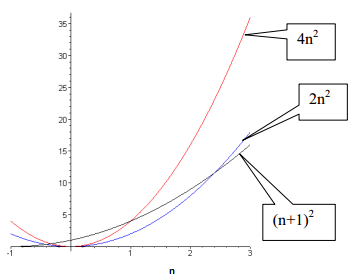
\includegraphics{MarcoTeorico/Imagenes/Cap2_1_1.png}
            \caption{Complejidad de los algoritmos.}      
            \label{fig:Cap2_1_1}
    \end{figure}    
    
    
\subsubsection{Orden de los algoritmos}
Por lo general la mayoría de los problemas tienen un parámetro de entrada que es el número de datos que hay que tratar, esto es, N. La cantidad de recursos del algoritmo es tratada como una función de N. 
Según \cite {[NIVIZI]} de esa manera puede establecerse un tiempo de ejecución del algoritmo que suele ser proporcional a una de las siguientes funciones:
\begin{itemize}
\item \textbf{$1$ (Tiempo de ejecución constante): }Significa que la mayoría de las instrucciones se ejecutan una cantidad  constante de tiempo.
\item \textbf{$logN$ (Tiempo de ejecución logarítmico): }Se puede considerar como una gran constante. La base del logaritmo (la más común es 2) cambia la constante, pero no demasiado. El programa es más lento cuanto más crezca \textit{N}, pero es inapreciable, pues \textit{logN} no se duplica hasta que \textit{N} llegue a $N^2$.
\item \textbf{$N$ (Tiempo de ejecución lineal): }Estos algoritmos puede resumirse como un bucle que se repite un número \textit{N} fijo de veces. Un caso en el que \textit{N} valga 40, tardará el doble que otro en que \textit{N} valga 20, pero si \textit{N} vale 30 tendría un tiempo intermedio de los \textit{N} anteriores. 
\item \textbf{$NlogN$ (Tiempo de ejecución en $NlogN$ ): }Es común encontrarlo en algoritmos como Quick Sort y otros del estilo divide y vencerás. Si N se duplica, el tiempo de ejecución es ligeramente mayor del doble.
\item \textbf{$N^2$ (Tiempo de ejecución cuadrático): }Suele ser habitual cuando se tratan pares de elementos de datos, como por ejemplo un bucle anidado doble. Si \textit{N} se duplica, el tiempo de ejecución aumenta cuatro veces. El peor caso de entrada del algoritmo Quick Sort se ejecuta en este tiempo.
\item \textbf{$N^3$ (Tiempo de ejecución cúbico): }Como ejemplo se puede dar el de un bucle anidado triple. Si \textit{N} se duplica, el tiempo de ejecución se multiplica por ocho.
\item \textbf{$2^N$ (Tiempo de ejecución exponencial): }No suelen ser muy útiles en la práctica por el elevado tiempo de ejecución. El problema de la mochila resuelto por un algoritmo de búsqueda exhaustiva es un ejemplo. Si N se duplica, el tiempo de ejecución crece de manera exponencial (de ahí el nombre).
\item \textbf{$n!$ (Tiempo de ejecución factorial): }La mayoría de ellos son intratables debido a que su exponente es igual al número de entradas que recibe. Si se aplica búsqueda exhaustiva a TSP, el tiempo de ejecución sería factorial.
\end{itemize}

En la figura \ref {fig:Ordenes_de_complejidad} se presenta una gráfica con el orden de crecimiento de cada uno de los conceptos en relación a su número de entradas y el tiempo que se tarda en resolverla.\\
\begin{figure}[hbtp]
    \centering
        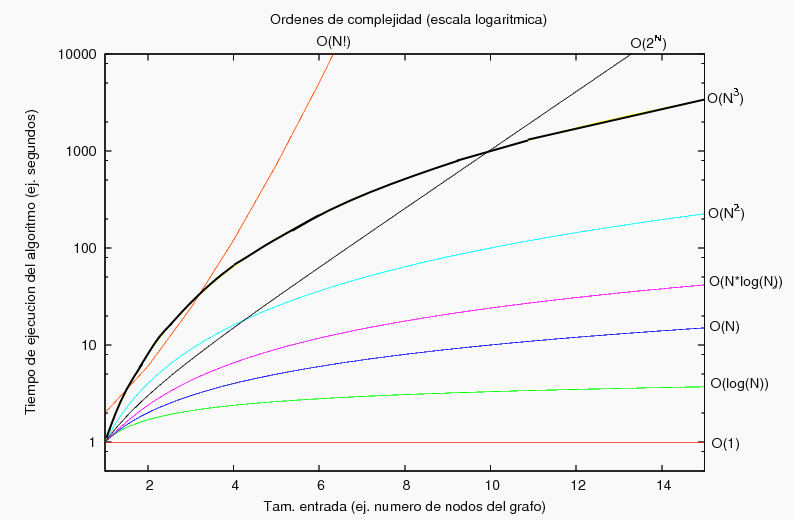
\includegraphics[width=0.8\textwidth]{MarcoTeorico/Imagenes/Ordenes_de_complejidad.png}
        \caption{Ordenes de complejidad.}      
        \label{fig:Ordenes_de_complejidad}
\end{figure}   

\subsubsection{Clasificación de los problemas}
Los problemas que tratan de resolver con algoritmos se pueden clasificar de diferentes perspectivas. De acuerdo con \cite{[MIGADA]} se tienen estas posibles clasificaciones:
\begin{enumerate}
\item 
\textbf{Por su naturaleza: }Se toma en cuenta la dificultad para resolver los algoritmos.
    \begin{itemize}
    \item \textbf{No computables: }Problemas que no admiten solución algorítmica, los problemas no computables que se basan en decisiones se llaman indecidibles.
    \item \textbf{Tratables:}Son los problemas para los cuales existen algoritmos de complejidad polinomial para resolverlos.
    \item \textbf{No tratables: }Son problemas que admiten solución y para los cuales de manera comprobada no pueden ser resueltos por algoritmos de complejidad polinomial.
    \end{itemize}
\item 
\textbf{Por el tipo de respuesta: }Es el determinar o responder SI o NO a una pregunta dada o solicitada.
\begin{itemize}
    \item \textbf{Problemas de decisión: }Es el determinar o responder SI o NO a una pregunta dada o solicitada.
    \item \textbf{Problemas de búsqueda: }Tienen como objetivo encontrar, en caso que exista, una estructura que verifique las restricciones del problema, dicha estructura es denominada de solución viable.
    \item \textbf{Problemas de optimización: }Comparte el mismo objetivo que los problemas de búsqueda pero este tipo en particular tiene que encontrar una estructura que optimice un criterio pre-definido es decir, debe encontrar la mejor solución. 
\end{itemize}
\item 
\textbf{Por su Tratabilidad: }Los problemas que admiten solución son clasificados de acuerdo a la complejidad que presentan los algoritmos para resolverlos.
\begin{itemize}
\item \textbf{La clase P: }Está constituida por todos los problemas que pueden ser resueltos por algoritmos de complejidad polinomial en una máquina convencional (máquina de Turing deterministica).
\item \textbf{La clase NP: }Es el conjunto de problemas que pueden ser resueltos en tiempo polinómico por una máquina de Turing no determinista, también contiene todos los problemas pertenecientes a las clases P, estos problemas tienen algoritmos ineficientes
\item \textbf{La clase NP-Completo: } Se dice que un problema es NP-completo si todos los problemas de la clase NP pueden reducirse a él, son los problemas más difíciles de la clase de problemas NP. Debido a la reducción, si se encuentra un algoritmo en tiempo polinomial para un problema NP-completo, se sabría que todos los problemas de la clase NP requieren un tiempo polinómico para resolverse.

\end{itemize}
\end{enumerate}

\subsubsection{Ejemplos de problemas NP-Completos}
Existen varios problemas NP-Completos, entre los más representativos se encuentran el problema de satisfacibilidad booleana y el problema del agente viajero 

\hspace*{1cm}\textbf{El problema de satisfacibilidad booleana:} De acuerdo a \cite{[Wilf]} el problema de satisfacibilidad booleana (SAT) fue el primer problema identificado como perteneciente a la clase de complejidad NP-completo en 1971. Según \cite{[Wilf]} el objetivo de SAT se enfoca a encontrar una asignación de valores a un conjunto de variables lógicas que son utilizadas para construir una fórmula lógica, de forma que dicha asignación produzca que ésta sea verdadera (una asignación satisfacible).\\
\hspace*{1cm}Normalmente la fórmula lógica se debe presentar en su forma normal conjuntiva (FNC) donde las variables lógicas se agrupan en claúsulas, que son una conjunción de literales. Como ejemplo considerando el siguiente conjunto de variables $x_1, x_2, x_3, x_4$ se tiene una fórmula lógica en su forma normal conjuntiva (FNC).
  $$(x_1 \lor \neg x_3 \lor x_4) \land (\neg x_2 \lor x_3 \lor \neg x_4)$$
\hspace*{1cm}Como se muestra en la tabla \ref{table:Cap2_1}  se verifican todas las combinaciones posibles de entradas en la que 10 de las 16 posibles generan una asignación verdadera lo que lo convierte en satisfacible. Por el contrario, si no existiera ninguna asignación que generara un resultado verdadero, entonces la fórmula sería insatisfacible.\\  

 \begin{table}[hbtp]
 \centering
    \caption{Ejemplo de satisfacibilidad booleana.} 
    \begin{tabular}{ | l | l | l | l | c |  }
    \hline
      \rowcolor[gray]{0.5}
       $x_1$ & $x_2$ & $x_3$ & $x_4$ & $(x_1\lor\neg x_3\lor x_4)\land(\neg x_2\lor x_3\lor\neg x_4) $ \\ \hline 
         V & V & V & V & V \\ \hline
         F & V & V & V & V \\ \hline
         V & F & V & V & V \\ \hline
         V & V & F & V & F \\ \hline
         V & V & V & F & V \\ \hline
         F & F & V & V & V \\ \hline
         F & V & F & V & F \\ \hline
         F & V & V & F & F \\ \hline
         V & F & F & V & V \\ \hline
         V & F & V & F & V \\ \hline
         V & V & F & F & F \\ \hline
         F & F & F & V & V \\ \hline
         F & F & V & F & F \\ \hline
         F & V & F & F & V \\ \hline
         V & F & F & F & V \\ \hline
         F & F & F & F & V \\ \hline
    \end{tabular}
    \label{table:Cap2_1}
    \end{table}
    \newpage
    
\textbf{Problema de la mochila:} 
Según \cite {[KARP]} el problema de la mochila es un problema que modela la situación de llenar una mochila limitada a cierta capacidad de peso y con cierta cantidad de objetos con diferentes pesos y valores cada uno. Los objetos que se pongan en la mochila deben de maximizar el valor total, sin superar el peso máximo permitido.\\
\hspace*{1cm}Como se puede ver en la figura \ref {fig:imagen_mochila} se muestra el ejemplo del problema de la mochila: dada una mochila con una capacidad de 15 kg para llenar con cajas de distinto peso y valor, se debe de elegir la mayor cantidad de cajas que pueden caber en la mochila sin exceder el peso permitido pero a la vez no sobre tanto espacio.

    \begin{figure}[hbtp]
        \centering
            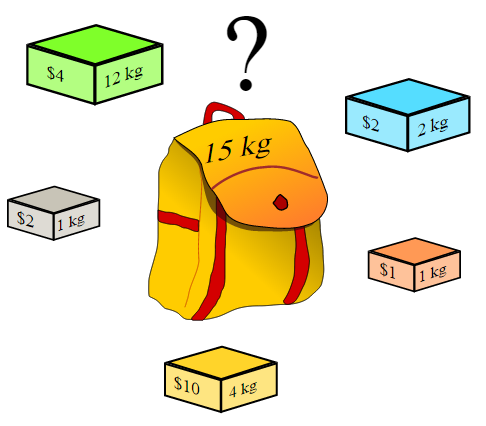
\includegraphics[width=0.5\textwidth]{MarcoTeorico/Imagenes/imagen_mochila.png}
            \caption{Ejemplo del problema de la mochila.}      
            \label{fig:imagen_mochila}
    \end{figure}   
    
Los datos del problema se pueden expresar en términos matemáticos.:
\begin{itemize}
\item Los objetos están numerados por el índice $i$ variando de $1$ a $N$ objetos (ítem).
\item De cada tipo de ítem se tienen $q_i$ ítems disponibles, donde $q_i$ es un entero positivo que cumple $1\leq q_i\leq\infty$.
\item Los números $w_{i}$ y $v_{i}$ representan el peso y el valor del número $i$. 
\item La capacidad de la mochila se denomina en esta fórmula $W$.
\item La solución al problema vendrá dado por la secuencia de variables $x_{n}$ donde el valor de $x_{i}$ indica cuantas copias se meterán en la mochila del tipo de ítem ${i}$
\end{itemize}
Con todo esto se puede formular matemáticamente de la siguiente forma:
%\begin{itemize}
%\item Maximizar $  \Sigma_{i=1}^{n}  v_{i} x_{i}$
%\item De tal manera que  $ \Sigma_{i=1}^{n}  w_{i} x_{i} \leq W $
%\item y $1\leq q_i\leq\infty$
%\end{itemize}

\begin{equation*}
\begin{aligned}
\text{maximizar } & \sum_{i=1}^N v_{i} x_{i} \\
\text{sujeto a }  & \sum_{i=1}^{n}  w_{i} x_{i} \leq W \\
                  & 1\leq q_i\leq\infty.
\end{aligned}
\end{equation*}  
    \subsection {Problema del agente viajero (TSP)}  
En TSP se tiene un número de nodos (ciudades, localidades, tiendas, empresas, etc.) que deben ser visitados por una entidad (persona, agente viajero, automóvil, avión, autobús, etc.), sin visitar 2 veces el mismo nodo. \\
\hspace*{1cm}Si se consideran 3 nodos (a, b y c) por visitar, entonces se tendrá una función de combinaciones sin repetición que se calcula con una función factorial ($n!$) es decir, se tendrán 6 posibles soluciones: abc, acb, bac, bca, cab, cba; para el caso de 4 nodos serian 24 combinaciones, para 10 nodos habría 3628800 combinaciones y así sucesivamente. En la figura \ref{fig:tsp1} se muestra otro ejemplo de los diferentes recorridos que puede dar un problema TSP, uno muestra un recorrido con un ineficiente resultado y otro con el resultado más eficiente.\\
    \begin{figure}[hbtp]
        \centering
            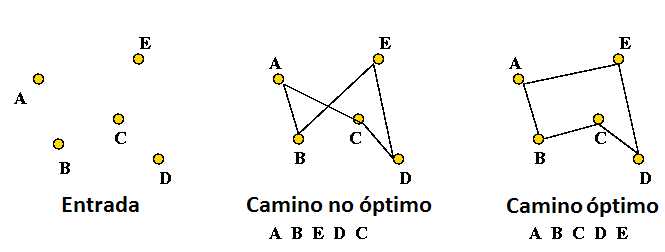
\includegraphics[width=1\textwidth]{MarcoTeorico/Imagenes/tsp1.png}
            \caption{Ejemplo de una instancia de TSP con 2 posibles soluciones.}                       
            \label{fig:tsp1}
    \end{figure} 
\hspace*{1cm}De acuerdo a \cite{[DANTZIG-RULKERSON]} la primera solución reportada para resolver una instancia del TSP fue en 1954, cuando Dantzig, Fulkerson y Johnson resolvieron una instancia de 49 ciudades.\\

\subsubsection{Características de TSP}
De acuerdo con \cite{[LENSTRA]}, TSP se encuentra clasificado como un problema de optimización combinatoria, es decir, en el problema en el que intervienen cierto número de variables donde cada variable puede tener N diferentes valores y cuyo número de combinaciones es de carácter factorial.\\
\hspace*{1cm}Para obtener una solución a una instancia del TSP se emplean diferentes métodos entre los cuales los principales se denominan heurísticas cuyo objetivo es generar soluciones de buena calidad en tiempos de cómputo mucho más pequeños (soluciones óptimas tiempo – respuesta). Las variables que han sido empleadas por la mayoría de los investigadores que dan solución a TSP son:

   \begin{itemize} 
      \item \textbf{Tiempo de recorrido entre ciudades:} Horas, minutos, días, semanas, etc.
      \item \textbf{Distancia de recorrido entre ciudades:} Metros, kilómetros, millas, milímetros, etc.
      \item \textbf{Costo de traslado:} Dinero, desgaste de las piezas, gasto de energía, etc.\\
   \end{itemize} 
   
\hspace*{1cm}Las variables que se pueden adoptar dependen de cada problema, por ejemplo:
   \begin{itemize} 
      \item \textbf{Circuitos electrónicos:} Cantidad de soldadura utilizada, menor espacio entre los puntos de soldadura de los circuitos, evitar el cruce entre las líneas de soldadura, tiempo de fabricación, distribución de los circuitos, entre otras.
      \item \textbf{Control de semáforos:} Número de semáforos (nodos), tiempo de traslado entre semáforos, cantidad de autos que pasan por un punto, entre otras variables.
      \item \textbf{Previsión del tránsito terrestre:} Puntos en una ciudad, cantidad de vehículos, tiempo de traslado, tipos de vehículos, horas pico, correlación entre variables, regresión lineal, etc.
      \item \textbf{Entrega de productos:} Peso de las entregas, número de entregas, nodos (domicilios) a visitar, recorridos, tiempos de traslado, tipo de vehículo, etc.
      \item \textbf{Estaciones de trabajo:} Secuencia de actividades, lugar de las herramientas (nodos), Tipo de herramientas, tiempo de uso, etc.
      \item \textbf{Edificación:} Puntos de edificación (construcciones), distancia entre las construcciones y los insumos, vehículos (grúas, camiones de volteo, etc.), cantidad de combustible que emplean, etc.
   \end{itemize} 

 
 \subsubsection {Algoritmo base}
 El TSP se puede modelar como un grafo cuyas aristas son los posibles caminos que puede seguir la entidad para visitar todos los nodos \cite{[ONCAN]}, y cuyo algoritmo se puede representar como en el pseudocódigo \ref{lst:codigo10}.\\
 
\begin{lstlisting}[language=HTML, caption=Algoritmo base del TSP., label=lst:codigo10]
* Definir el número de nodos, su posición y el costo por cada arista (i, j) donde i = ciudad 1 y j = ciudad 2.
* Elegir el nodo inicial i.
* Si el nodo más cercano no se ha visitado, visitar nodo j.
* Actualizar lista de nodos visitados.
* CostoTotal = CostoTotal + costo(i, j).
* Nodo i = nodo j.
* Repetir punto 3 hasta haber visitado todos los nodos.
\end{lstlisting}    
     
\subsubsection {Aplicaciones}
El TSP se puede emplear en cualquier situación que requiere seleccionar nodos en cierto orden que reduzca los costos:

\begin{itemize}
  \item \textbf{Reparto de productos:} Mejorar una ruta de entrega para seguir la más corta.
  \item \textbf{Transporte:} Mejorar el recorrido de caminos buscando la menor longitud.
  \item \textbf{Robótica:} Resolver problemas de fabricación para minimizar el número de desplazamientos al realizar una serie de perforaciones en un circuito impreso.
  \item \textbf{Turismo y agencias de viajes:} Aun cuando los agentes de viajes no tienen un conocimiento explícito del TSP, las compañías dedicadas a este giro utilizan un software que hace todo el trabajo. Estos paquetes son capaces de resolver instancias pequeñas del TSP.
  \item \textbf{Horarios de transportes laborales y/o escolares:} Estandarizar los horarios de los transportes es claramente una de sus aplicaciones, tanto que existen empresas que se especializan en ayudar a las escuelas a programarlos para optimizarlos en base a una solución del TSP.
  \item \textbf{Inspecciones a sitios remotos:} Ordenar los lugares que deberá visitar un inspector en el menor tiempo.
  \item \textbf{Secuencias:} Se refiere al orden en el cual n trabajos tienen que ser procesados de tal forma que se minimice el costo total de producción.
\end{itemize}
   
\subsubsection {Técnicas de solución}
El TSP puede resolverse de diferentes maneras:

\begin{itemize}
    \item \textbf{Enumeración de todas las soluciones factibles:} Es decir, listar todas las posibles soluciones al problema, calcular sus costos asociados e identificar, por comparación, cuál es la solución con el costo más conveniente.
 \item \textbf{Métodos exactos:} Intentan descartar familias enteras de posibles soluciones, tratando así de acelerar la búsqueda y llegar a una óptima. Los que más se usan para resolver el TSP son Ramificación y Acotamiento, y Ramificación y Corte.
 \item \textbf{Heurísticas:} Son métodos obtienen buenas soluciones en tiempos de cómputo muy cortos, aunque sin garantizar la solución única.
\end{itemize}

\hspace*{1cm}En la actualidad investigadores han propuesto diferentes estrategias para dar solución a TSP, de las cuales se pueden mencionar algunas técnicas empleadas:

\begin{itemize}
\item \textbf{Algoritmos genéticos:} La solución consiste en encontrar un individuo cuya combinación de genes (cada gen es una variable), den solución al problema de visitar todas las ciudades una vez. Otra solución es que cada gen es una ciudad y cuyo orden dependerá del orden en que serán visitadas.
\item \textbf{Redes neuronales:} Una red neuronal simula las conexiones entre los nodos (lugares por visitar), y cada recorrido por las diferentes neuronas genera al final un camino que involucra el tour por todas las ciudades visitadas una sola vez.
\item \textbf{Colonia de hormigas (ACO):} Las hormigas encuentran el camino más corto entre 2 puntos; para TSP, se considera el punto de inicio como el punto final, de esta manera, las hormigas deben recorrer todas las ciudades en un circuito, sin pasar 2 veces por la misma ciudad.
\item \textbf{Búsqueda Tabú:} Consiste en buscar el vecino próximo cuyos costos de traslado del nodo actual al siguiente sea el de menor costo en cuanto al uso de recursos.
\item \textbf{Combinación de propuestas:} Las técnicas de Inteligencia Artificial se pueden combinar para crear metaheurísticas conformando diferentes soluciones tales como: algoritmos genéticos con redes neuronales.
\end{itemize}

 
    \subsection {Metaheurísticas}  
El siguiente tema abordara sobre las metaheurísticas, sus características y principales ejemplos.
\subsubsection {Concepto de heurística}  
Según \cite{[ZANAEVA]} un heurístico es un “procedimiento simple, a menudo basado en el sentido común, que se supone que ofrecerá una buena solución (aunque no necesariamente la óptima) a problemas difíciles, de un modo fácil y rápido”. Las heurísticas se utilizan, por ejemplo, cuando no existe un método exacto de resolución, cuando existe un método exacto que consume mucho tiempo para ofrecer la solución óptima, cuando existen limitaciones de tiempo o como paso intermedio para obtener una solución inicial para la aplicación de otra técnica. Según \cite {[SILVER]} se propone la siguiente clasificación de métodos de resolución mediante heurísticas:
\begin{itemize}
\item \textbf{Métodos constructivos: } Se caracterizan por construir una solución definiendo diferentes partes de ella en sucesivos pasos.
\item \textbf{Métodos de descomposición: } Dividen el problema en varios más pequeños y la solución se obtiene a partir de la solución de cada uno de estos.
\item \textbf{Métodos de reducción: } Tratan de identificar alguna característica de la solución que permita simplificar el tratamiento del problema.
\item \textbf{Métodos de manipulación del modelo: } Obtienen una solución del problema original a partir de otra de otro problema simplificado (con menos restricciones, linealizando el problema, etc.)
\item \textbf{Métodos de búsqueda por entornos: } En las que se parte de una solución inicial a la que se realizan modificaciones en sucesivas iteraciones para obtener una solución final. En cada iteración existe un conjunto de soluciones vecinas candidatas a ser nueva solución en el proceso. En este grupo se encuadran las técnicas metaheurísticas.
\end{itemize}

\subsubsection {Características principales de las metaheurísticas} 

Las técnicas metaheurísticas son procedimientos de búsqueda que tampoco garantizan la obtención del óptimo del problema considerado y que también se basan en la aplicación de reglas relativamente sencillas.\\ 
\hspace*{1cm}A diferencia de las heurísticas, las técnicas metaheurísticas tratan de escapar de óptimos locales orientando la búsqueda en cada momento dependiendo de la evolución del proceso de búsqueda. \cite{[SADIQBIB]} dice que las metaheurísticas tienen como características:
\begin{itemize}
\item \textbf{Ser ciegas: } No saben si llegan a la solución óptima. Por lo tanto, se les debe indicar cuándo deben detenerse.
\item \textbf{Ser algoritmos de aproximación:} Por tanto no garantiza la obtención de la solución óptima.
\item \textbf{Aceptan ocasionalmente soluciones ineficientes: } Sin embargo pueden ser de utilidad para acceder a nuevas regiones y escapar de óptimos locales.
\item \textbf{Ser relativamente sencillos:} Todo lo que se necesita es una representación
adecuada del espacio de soluciones, una solución inicial (o un conjunto de ellas) y un mecanismo para explorar el campo de soluciones.
\item \textbf{Ser generales:} Prácticamente se pueden aplicar en la resolución de cualquier problema de optimización de carácter combinatorio. Sin embargo, la definición de la técnica será más o menos eficiente en la medida en que las operaciones tengan relación con el problema considerado.
\item \textbf{Ser impredecibles:} La regla de selección depende del instante del proceso y de la historia hasta ese momento. Si en dos iteraciones determinadas la solución es la misma, la nueva solución de la siguiente iteración no tiene por qué ser necesariamente la misma.
\end{itemize}

\hspace*{1cm}Aunque las soluciones que ofrecen los técnicas metaheurísticas no son las óptimas y, en general, ni siquiera es posible conocer la proximidad de las soluciones al óptimo, permiten estudiar problemas de gran complejidad de una manera sencilla y obtener soluciones suficientemente buenas en tiempos razonables.\\

De acuerdo a \cite{[BLUMROLI]} las metaheurísticas se pueden clasificar según:
\begin{itemize}
    \item Si están inspiradas en procesos naturales
    \item Si son dinámicas o estáticas
    \item Si manejan memoria
    \item Si están basados en poblaciones y manejan varias soluciones por proceso
    \item Si utilizan técnicas de agrupamiento 
\end{itemize}

\subsubsection {Algoritmo voraz (Greedy)}
Los algoritmos voraces (del inglés greedy) reciben esta denominación por las siguientes razones según \cite{[CORMENL]}:
\begin{itemize}
\item Siempre escoge el mejor candidato para formar parte de la solución: Aquel que tenga mejor valor de la función objetivo, lo que constituye el cumplimiento de cierto criterio goloso de selección.
\item Esta elección es única e inmodificable dado que no analiza más allá los efectos de haber seleccionado un elemento como parte de la solución. No deshacen una selección ya realizada: una vez incorporado un elemento a la solución permanece hasta el final y cada vez que un candidato es rechazado, lo es permanentemente.
\end{itemize}
\hspace*{1cm}Se sabe sin embargo la calidad de los algoritmos voraces está en relación con las características de las instancias que pretenden resolver: puede arrojar muy buenos resultados para determinadas instancias del problema pero para otras no. Otro inconveniente que presentan es que se estancan en óptimos locales de las funciones que pretenden optimizar y quizá no analizan vecindades más allá del criterio goloso por lo que pueden estar dejando de considerar al óptimo global.

A continuación el pseudocodigo \ref{lst:PseudocodigoGreedy} que muestra cómo funciona:
\begin{lstlisting}[language=C++, caption=Pseudocódigo base para el algoritmo greedy., label=lst:PseudocodigoGreedy]
/* Algoritmo de Greedy*/
Inicio
  S=Solucion Inicial
  Mientras (Condición establecida){
  S´= Se genera una solución nueva en base a la inicial
    if (S´> S){
        S = S´
    }
  }
  retorno S
Fin;
\end{lstlisting}

\hspace*{1cm}A diferencia de otros algoritmos éste no almacena soluciones adicionales y entre sus virtudes se encuentra en la simplicidad que tiene y por tanto, menor manejo de recursos, sin embargo su defecto se encuentra en el hecho de que no toma decisiones alejadas de la solución inicial, si ésta no cumple con su objetivo se deshace el cambio anterior y continua con el procedimiento hasta que cumpla con la condición establecida.\\

\subsubsection {Búsqueda local}  
Según \cite{[ADPEREZ]}, la idea básica de los algoritmos de búsqueda local es iniciar con una solución inicial ya sea generada aleatoriamente o hallada con algún otro algoritmo; una vez obtenida se realiza una transformación aleatoria de sus valores para mejorar la solución. Dicha transformación se repite hasta que ya no se pueda mejorar más la solución o bien, que cumpla con ciertas condiciones.\\
\hspace*{1cm}En la figura \ref{fig:EXPLOCAL.png} se puede ver un ejemplo de una gráfica formada por las ciudades $(v, x, y, z)$, analizando la ruta de la izquierda se puede crear una nueva ruta reemplazando dos caminos que comprenden los puntos $(x,y)$ y $(v,z)$ haciendo los caminos $(x,v)$ y $(y,z)$ produciendo un nuevo tour que es el que se puede apreciar a la derecha de la misma imagen.\\
%\hspace*{1cm}La vecindad de I consiste de todas aquellas soluciones que se obtienen haciendo el reemplazo de pares arcos.\\
%¿Cuántos vecinos tiene I si consiste de n ciudades vecinas?La respuesta viene siendo un problema del tipo O($N^2$) ya que cada ciudad tiene una probabilidad de 1 de 7 para conectarse con la ruta más óptima.\\

    \begin{figure}[hbtp]
        \centering
            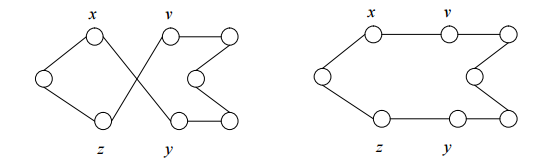
\includegraphics[width=0.6\textwidth]{MarcoTeorico/Imagenes/EXPLOCAL.png}
            \caption{Ejemplo de búsqueda local aplicado al TSP.}                       
            \label{fig:EXPLOCAL.png}
    \end{figure} 
    
\subsubsection {Recocido simulado}  

Recocido Simulado (SA por sus siglas en inglés) de acuerdo a \cite{[METROPOLIS]} es un método de optimización inspirado en el proceso de templado de metales. El algoritmo de recocido simulado es un método iterativo que inicia con una perturbación de cierto estado $s$. Mediante un proceso particular genera un estado vecino $s'$ al estado actual. Si la energía, o evaluación, del estado $s'$ es menor que la del estado $s$, se cambia el estado $s$ por $s'$. Si la evaluación de $s'$ es mayor que la de $s$ entonces se puede elegir $s'$ en lugar de $s$ con una cierta probabilidad que depende de las diferencias de las evaluaciones $\Delta f = f(s)-f(s') $ y de la temperatura actual del sistema $T$. La posibilidad de elegir un estado peor al actual es lo que le permite a SA salir de óptimos locales para poder llegar a los óptimos globales. La probabilidad de aceptar elegir un peor estado normalmente se calcula por la distribución de Boltzmann: $$ P(\Delta f, T) = e ^{\Delta f/T} $$
\hspace*{1cm}La cualidad de SA es que la temperatura va disminuyendo gradualmente conforme avanza la simulación. El código \ref{lst:recocidosimulado} representa una versión general del algoritmo de recocido simulado:\\

\begin{lstlisting}[language=HTML, caption=Pseudocódigo base para el algoritmo de recocido simulado., label=lst:recocidosimulado]
s := GeneraUnaSolucionInicial();
T := T0; g := 0;
mientras (CondicionesParoNoActivas(g, T)) hacer
    s' := Toma Un VecinoAleatorioDe(s);
    si ( f(s') < f(s))
        s := s';
    No
    //se usara la fórmula de temperatura
        si (Random(0, 1.0) < exp((f(s) - f(s'))/T)) 
            s := s';
        fin si;
    fin si;
g := g + 1; T := Actualiza(g, T);
fin mientras
\end{lstlisting}

%En la figura \ref{fig:RecocidoSimulado} se presenta un ejemplo propuesto de \cite{[GRANVILLE]}:  El problema consiste en disponer los píxeles en la imagen de tal manera que se minimice una función de energía potencial que causa que los colores similares se atraigan a distancias cortas y se repelan a distancias largas. En cada iteración se intercambian las posiciones de dos píxeles adyacentes. La imagen de la izquierda es obtenida con un protocolo de enfriado rápido, en el que la temperatura desciende rápidamente, y la de la derecha, con un protocolo lento, equiparables a los procesos de formación de sólidos amorfos y cristalinos respectivamente.

%    \begin{figure}[hbtp]
%        \centering
%            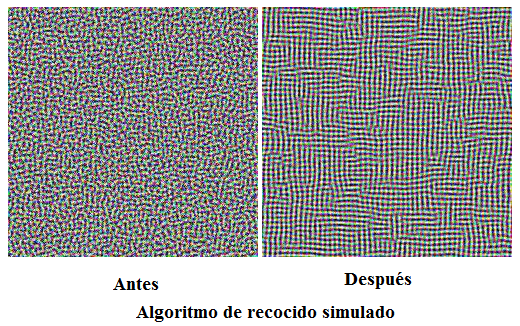
\includegraphics[width=0.6\textwidth]{MarcoTeorico/Imagenes/RecocidoSimulado.png}
%            \caption{Ejemplo de un problema de alineamiento de píxeles aplicando recocido simulado.}                       
%            \label{fig:RecocidoSimulado}
%    \end{figure} 


\subsubsection {Algoritmo genético}

Los algoritmos genéticos (AG) son métodos adaptativos que están basados en la teoría evolutiva de Darwin y la teoría genética de Mendel. En la naturaleza los individuos de una población compiten entre sí en la búsqueda de recursos tales como comida, agua y refugio. Incluso los miembros de una misma especie compiten a menudo en la búsqueda de un compañero. Aquellos individuos que tienen más éxito en sobrevivir y en atraer compañeros tienen mayor probabilidad de generar un gran número de descendientes.\\
\hspace*{1cm}Como se puede ver en la figura \ref{fig:agenetico} se tiene un grupo de individuos representado por círculos de colores, en algún momento 2 de estos círculos se juntarán y darán origen a un nuevo círculo, aunque posean algunas de las mismas características que sus padres es un ser único, este nuevo individuo se integrará al grupo y continuará su ciclo.

    \begin{figure}[hbtp]
        \centering
            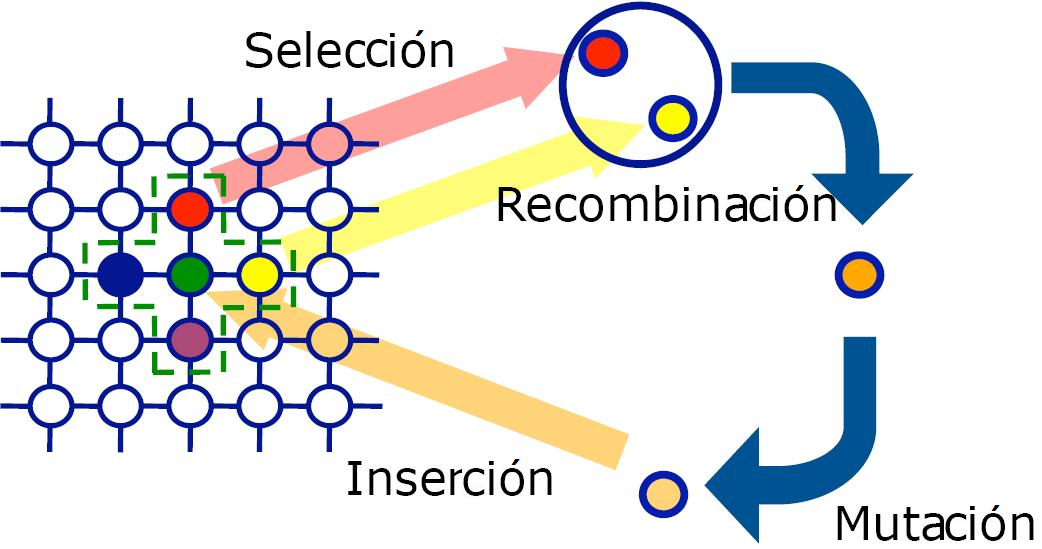
\includegraphics[width=0.7\textwidth]{MarcoTeorico/Imagenes/agenetico.png}
            \caption{Ejemplo de cómo funciona el algoritmo genético.}                       
            \label{fig:agenetico}
    \end{figure} 
    
\hspace*{1cm}A continuación se presentará un resumen basado en la idea general del algoritmo genético según \cite{[HOLLAND]}, \cite{[REEVES]}, \cite{[MICHALEWICZ]}, \cite{[DAVIS]},  \cite{[GOLDBERG]}. Las soluciones del problema se representan como un conjunto de parámetros llamados genes, los cuales agrupados forman un grupo de valores llamado cromosoma; el alfabeto que se usa para tratar con estos problemas puede ser cualquiera, pero para la siguiente explicación se usará el 1 y el 0. El conjunto de parámetros representando un cromosoma en específico se denomina fenotipo, el fenotipo contiene la información requerida para construir una solución el cual se refiere como genotipo.\\
\hspace*{1cm}La función de adaptación debe ser diseñada para cada problema de manera específica. Dado un cromosoma particular, la función de adaptación le asigna un valor numérico que se supone refleja el nivel de adaptación al problema del individuo representado por el cromosoma. Durante la fase reproductiva se seleccionan los individuos de la población para cruzarse y producir descendientes que constituirán, una vez mutados, la siguiente generación de individuos. La selección de padres se efectúa al azar usando un procedimiento que favorezca a los individuos mejor adaptados, ya que a cada individuo se le asigna una probabilidad de ser seleccionado que es proporcional a su función de adaptación. Es decir, los individuos bien adaptados se escogerán probablemente varias veces por generación, mientras que los pobremente adaptados al problema no se escogerán más que de vez en cuando. Una vez seleccionados los 2 padres, sus cromosomas se combinan utilizando habitualmente los operadores de cruce y mutación. Las formas básicas de dichos operadores se describen a continuación: 

\begin{itemize}
    \item El operador de cruce toma a los 2 padres seleccionados y divide sus genes en una posición escogida al azar para producir dos pares de cromosomas cada uno. Después se intercambian los cromosomas finales para crear una solución nueva (Figura \ref{fig:Codigo-genetico1}). Ambos descendientes heredan genes de cada uno de los padres. Este operador se conoce como operador de cruce basado en un punto.
    \item El operador de mutación se aplica a cada hijo de manera individual y consiste en la alteración aleatoria (normalmente con probabilidad pequeña) de cada gen componente del cromosoma.
\end{itemize}

\begin{figure}[hbtp]
    \centering
        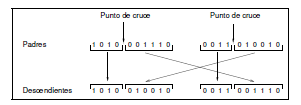
\includegraphics[width=0.7\textwidth]{MarcoTeorico/Imagenes/Codigo-genetico1.png}
        \caption{Operador de cruce basado en un punto.}                       
        \label{fig:Codigo-genetico1}
\end{figure} 
 
\hspace*{1cm}La figura \ref{fig:Codigo-genetico2} muestra la mutación del quinto gen del cromosoma.  Aunque el operador de cruce es más importante que el operador de mutación por proporcionar una exploración rápida del espacio de búsqueda, el operador de mutación asegura que ningún punto del espacio de búsqueda tenga probabilidad cero de ser examinado y es importante para asegurar la convergencia de un AG.

   \begin{figure}[hbtp]
        \centering
            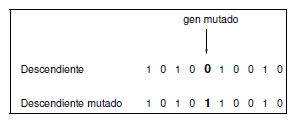
\includegraphics[width=0.7\textwidth]{MarcoTeorico/Imagenes/Codigo-genetico2.png}
            \caption{Operador de mutación.}                       
            \label{fig:Codigo-genetico2}
    \end{figure} 
    
\hspace*{1cm}El código \ref{lst:AlgoritmoGenetico} representa una versión general del algoritmo genético:\\

\begin{lstlisting}[language=C++, caption=Pseudocódigo base para el algoritmo algoritmo genético., label=lst:AlgoritmoGenetico]
/* Algoritmo Genético Simple */
Generar una población inicial().
Computar la función de evaluación de cada individuo().
MIENTRAS(NOT Terminado){
    /* Producir nueva generación */
    Ciclo (Tamaño población/2){
     /*Ciclo Reproductivo */
        1.-Seleccionar dos individuos de la anterior generación para el cruce (probabilidad de selección proporcional a la función de evaluación del individuo);
        2.-Cruzar con cierta probabilidad los dos individuos obteniendo dos descendientes;
        3.-Mutar los dos descendientes con cierta probabilidad. Computar la función de evaluación de los dos descendientes mutados;
        4.-Insertar los dos descendientes mutados en la nueva generación;
    }
}
SI( la población ha convergido) {
    Terminado := TRUE
}
Fin;

\end{lstlisting}
    
    \subsection {Autómata finitos}  
Según \cite{[PINOCHO]} un autómata finito (máquina de estados finitos), es un modelo computacional que realiza cómputos en forma automática sobre una entrada para producir una salida.\\
\hspace*{1cm}Este modelo está conformado por un alfabeto, un conjunto de estados y un conjunto de transiciones entre dichos estados. Su funcionamiento se basa en una función de transición, que recibe a partir de un estado inicial una cadena de símbolos pertenecientes al alfabeto (la entrada), y que va leyendo dicha cadena a medida que el autómata se desplaza de un estado a otro, para finalmente detenerse en un estado final o de aceptación, que representa la salida.\\
\hspace*{1cm}La finalidad de los autómatas finitos es la de reconocer lenguajes regulares. Formalmente, un autómata finito es una 5-tupla $<Q, \Sigma, q0, \delta, F>$ donde:
    \begin{itemize}
        \item \textbf{$Q$} es un conjunto finito de estados.
        \item \textbf{$\Sigma$} es un alfabeto finito de símbolos.
        \item \textbf{$q0$} es el estado inicial en Q.
        \item \textbf{$\delta$} es la relación de transiciones de la forma $<qi,x,qj>$ con $qi$ y $qj$ como estados de $Q$ y $x$, símbolo de $\Sigma$ ó puede ser también la cadena vacía.
        \item \textbf{$F$} es el conjunto de estados finales o de aceptación y (evidentemente) subconjunto de $Q$.
    \end{itemize}
    
%\hspace*{1cm}Los autómatas que se abarcara en este tema serán autómatas finitos deterministas y los autómatas finitos no deterministas.\\

\subsubsection {Autómatas finitos deterministas}  
Según \cite{[PINOCHO2]} un autómata finito determinista (AFD) es un autómata finito que además es un sistema determinista; es decir, para cada estado $q \in Q$ en que se encuentre el autómata, y con cualquier símbolo $\alpha \in \Sigma$ del alfabeto leído, existe siempre a lo más una transición posible $\delta(q,a)$. En la figura \ref{fig:AFN_CONVERTIDO.png} se puede apreciar un ejemplo de un AFD que consta de los elementos mencionados en la lista anterior:

\begin{itemize}
\item \textbf{$Q$}: (q0,q1,q2).
\item \textbf{$\Sigma$}: (a,b).
\item \textbf{$q0$}: (q0).
\item \textbf{$\delta$}: es la relación de transiciones que se muestran en la tabla \ref{table:AFN_CONVERTIDO}.
\item \textbf{$F$}: (q2).
\end{itemize}

\begin{table}[hbtp]
\centering
   \caption{Ejemplo de transiciones de un AFD.}
   \begin{tabular}{ | l | l | l |}
   \hline
     \rowcolor[gray]{0.5}
          &   a  &  b   \\ \hline
       q0 &  q1  & q0   \\ \hline   
       q1 &  q1  & q2   \\ \hline
      *q2 &  q1  & q0   \\ \hline
   \end{tabular}
   \label{table:AFN_CONVERTIDO}
\end{table}

    \begin{figure}[hbtp]
        \centering
            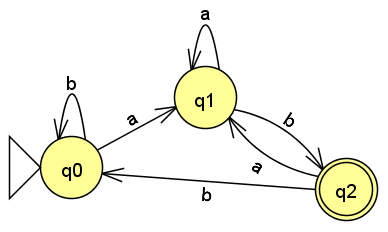
\includegraphics[width=0.5\textwidth]{MarcoTeorico/Imagenes/AFN_CONVERTIDO.png}
            \caption{Ejemplo de autómata finito determinista.}     
            \label{fig:AFN_CONVERTIDO.png}
    \end{figure} 

\hspace*{1cm}El autómata en cuestión acepta solamente las cadenas de símbolos que terminen con $ab$, una vez que ya no existen más caracteres y éste cae en el estado $q2$ (aquél que está en doble círculo) significa que es una cadena válida para el autómata.\\
\hspace*{1cm}En un AFD no pueden darse ninguno de estos dos casos:
    \begin{itemize}
        \item Que existan dos transiciones del tipo $\delta(q,a)=q1$ y $\delta(q,a)=q2$, siendo $q1 \neq q2$;
        \item Que existan transiciones del tipo $\delta(q,\epsilon)$, salvo que q sea un estado final, sin transiciones hacia otros estados.
    \end{itemize}    
\subsubsection {Autómatas finitos no deterministas}      
Según \cite{[PINOCHO3]} un autómata finito no determinista (AFND) es aquél que, a diferencia de los autómatas finitos deterministas, posee al menos un estado $ q \in Q$, tal que para un símbolo $\alpha \in \Sigma$ del alfabeto, existe más de una transición $\delta(q,a)$ posible. Haciendo la analogía con los AFDs, en un AFND puede darse cualquiera de estos dos casos:
    \begin{itemize}
        \item Que existan transiciones del tipo $\delta(q,a)=q1$ y $\delta(q,a)=q2$, siendo $q1 \neq q2$;
        \item Que existan transiciones del tipo $\delta(q,\epsilon)$, siendo q un estado no-final, o bien un estado final pero con transiciones hacia otros estados.
        \item Cuando se cumple el segundo caso, se dice que el autómata es un autómata finito no determinista con transiciones vacías o transiciones $\epsilon$ (abreviado AFND-$\epsilon$). Estas transiciones permiten al autómata cambiar de estado sin procesar ningún símbolo de entrada.
        \item También hacen transiciones $\epsilon$ que son aquellas donde se mueve a otro estado sin hacer nada, siempre y cuando el estado actual lo indique.
    \end{itemize}
\hspace*{1cm}Haciendo un ejemplo con el autómata de la figura \ref{fig:AFN_CONVERTIDO.png} se puede observar que se puede hacer un AFND con la misma cadena de aceptación:

    \begin{figure}[hbtp]
        \centering
            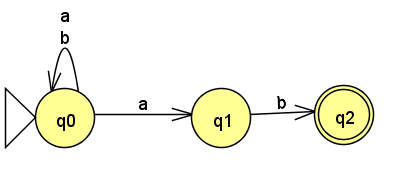
\includegraphics[width=0.5\textwidth]{MarcoTeorico/Imagenes/AFN.png}
            \caption{Ejemplo de autómata finito no determinista.}     
            \label{fig:AFN.png}
    \end{figure} 
    
\hspace*{1cm}Como se puede observar en la figura \ref{fig:AFN.png} tiene una menor cantidad de transiciones, como se puede ver en la tabla \ref{table:AFN} el estado $q0$ produce 2 estados en la transición $a$, una que lleva al estado $q1$ y otra que lleva nuevamente al estado $q0$, es este momento en el que se hacen 2 procesos por separado, cada uno siguiendo un distinto estado así sucesivamente hasta que termine la cadena.

\begin{table}[hbtp]
\centering
   \caption{Ejemplo de transiciones de un AFND.}
   \begin{tabular}{ | l | l | l |}
   \hline
     \rowcolor[gray]{0.5}
          &   a     &  b   \\ \hline
       q0 &  q0,q1  & q0   \\ \hline   
       q1 &         & q2   \\ \hline
      *q2 &         &      \\ \hline
   \end{tabular}
   \label{table:AFN}
\end{table}

\hspace*{1cm}Como se menciona anteriormente, las transiciones $\epsilon$ son, de acuerdo a \cite{[PINOCHO4]}, transiciones que permiten ir a otro estado sin necesidad de un símbolo. La figura \ref{table:EjemploAFND} muestra un autómata que acepta la expresión regular ($0*1*2*$):

 \begin{itemize}
\item \textbf{$Q$}: (q0,q1,q2).
\item \textbf{$\Sigma$}: (0,1,2).
\item \textbf{$q0$}: (q0).
\item \textbf{$\delta$}: es la relación de transiciones que se muestran en la tabla \ref{table:EjemploAFND}.
\item \textbf{$F$}: (q2).
\end{itemize}

 \begin{table}[hbtp]
\centering
   \caption{Ejemplo de AFND con transición $\epsilon$.}
   \begin{tabular}{ | l | l | l | l | l |}
   \hline
     \rowcolor[gray]{0.5}
          &  0  &  1  &  2  & $\epsilon$   \\ \hline
       q0 & q0  &     &     & q1           \\ \hline   
       q1 &     & q1  &     & q2           \\ \hline
      *q2 &     &     & q2  &              \\ \hline
   \end{tabular}
   \label{table:EjemploAFND}
\end{table}

 \begin{figure}[hbtp]
    \centering
        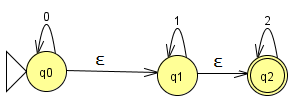
\includegraphics[width=0.5\textwidth]{MarcoTeorico/Imagenes/aufnd_b.png}
        \caption{Ejemplo de AFND con transición $\epsilon$.}     
        \label{fig:aufnd.png}
\end{figure} 

\hspace*{1cm}Como se puede observar en este ejemplo, la transición $\epsilon$ permite saltar de un estado a otro sin usar un símbolo; en caso de que el siguiente estado no posea ninguna transición con el símbolo actual puede tomar (en caso de que tenga) la transición $\epsilon$ actuando como un sustituto. También se puede dar el caso de que exista una transición $\epsilon$ y una transición con el símbolo actual. En este caso se generan 2 procesos en paralelo para satisfacer ambas transiciones. En el siguiente ejemplo se puede explicar lo mencionado anteriormente:

 \begin{itemize}
\item \textbf{$Q$}: (q0,q1,q2,q3).
\item \textbf{$\Sigma$}: (a,b).
\item \textbf{$q0$}: (q0).
\item \textbf{$\delta$}: es la relación de transiciones que se muestran en la tabla \ref{table:EjemploAFND2}.
\item \textbf{$F$}: (q2).
\end{itemize}

\begin{table}[hbtp]
\centering
   \caption{Segundo ejemplo de un AFND con transición $\epsilon$.}
   \begin{tabular}{ | l | l | l | l |}
   \hline
     \rowcolor[gray]{0.5}
          & a &  b     & $\epsilon$   \\ \hline
       q0 &   & q1,q3  & q0          \\ \hline   
       q1 &   & q2     &             \\ \hline  
      *q2 &   &        &             \\ \hline  
       q3 &   &        & q2          \\ \hline  
   \end{tabular}
   \label{table:EjemploAFND2}
\end{table}

 \begin{figure}[hbtp]
    \centering
        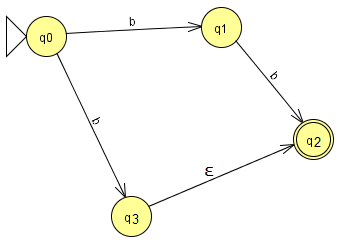
\includegraphics[width=0.5\textwidth]{MarcoTeorico/Imagenes/AFN2_b.png}
        \caption{Segundo ejemplo de AFND con transición $\epsilon$.}     
        \label{fig:AFN2.png}
\end{figure} 

\hspace*{1cm}En este ejemplo se puede observar que este autómata acepta solamente las cadenas $b$ y $bb$. En el estado inicial la transición $b$ lleva a dos estados distintos, en ese momento se tomarán en cuenta los 2 estados $q1$ y $q3$ donde el estado $q1$ podrá llegar al estado de aceptación $q2$ si encuentra otra cadena $b$ mientras que el estado $q3$ podrá llegar a su estado de aceptación si no existe otra cadena (que se interpreta con la transición $\epsilon$).\\  
    \subsection {Técnicas de agrupamiento (Clustering)}  
Según \cite{[PASPLASA]} y \cite{[PASPLASA2]} el problema del agrupamiento (también conocido como clustering) puede definirse como sigue: dados n puntos en un espacio n-dimensional, particionar los mismos en k grupos tales que los puntos dentro de un grupo son más similares que cada uno a los de los otros grupos; dicha similaridad se mide atendiendo a alguna función de distancia o alguna otra función. En la figura \ref{fig:Cap2_3_2_1} aparece un ejemplo del agrupamiento.\\

    \begin{figure}[hbtp]
        \centering
            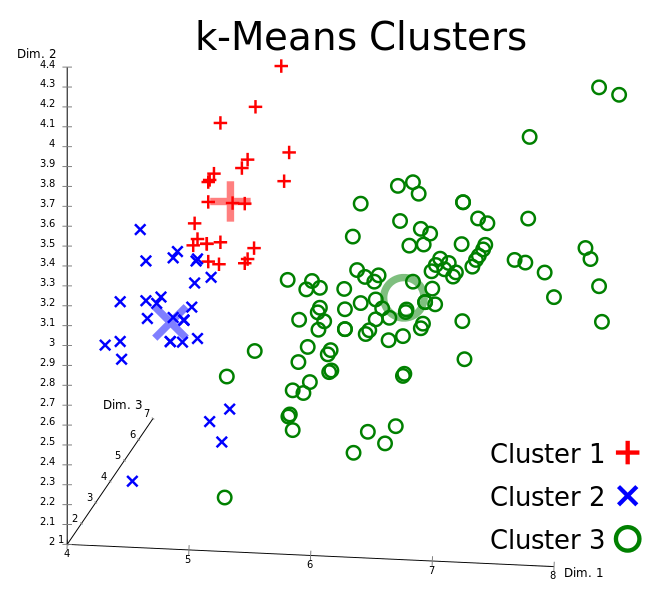
\includegraphics[width=0.6\textwidth]{MarcoTeorico/Imagenes/imagencluster.png}
            \caption{Ejemplo de agrupamiento.}                       
            \label{fig:Cap2_3_2_1}
    \end{figure} 
    
\hspace*{1cm}Los métodos de agrupamiento se pueden dividir en paramétricos y no paramétricos. Entre los métodos de agrupamiento paramétricos se encuentran las mixturas finitas, éstas son una poderosa herramienta para modelar densidades de probabilidad de conjuntos de datos univariados y multivariados, modelan observaciones las cuales se asume que han sido producidas por un conjunto de fuentes aleatorias alternativas e infieren los parámetros de estas fuentes para identificar qué fuente produjo cada observación, lo que lleva a un agrupamiento del conjunto de observaciones. Los métodos de agrupamiento no paramétricos pueden dividirse en tres grupos fundamentales: jerárquicos, particionales y basados en densidad.

 \subsubsection {Algoritmos jerárquicos}
Según \cite{[PASPLASA]} los algoritmos jerárquicos son aquellos en los que se va particionando el conjunto de datos por niveles, de modo que en cada nivel generalmente se unen o dividen dos grupos del nivel anterior de acuerdo al tipo de algoritmo: aglomerativo o divisivo. Según \cite{[DUHASTO]} las estrategias jerárquicas más conocidas son:
 \begin{itemize}
 \item \textbf{Single Link (SL): }En cada paso se unen los dos grupos cuyos elementos más cercanos 
tienen la mínima distancia.
 \item \textbf{Average Link (AL): }En cada paso se unen los dos grupos que tienen la mínima distancia promedio entre sus puntos.
 \item \textbf{Complete Link (CL): }En cada paso se unen los dos grupos tal que su unión tiene el diámetro mínimo o los dos grupos con la menor distancia máxima entre sus elementos.  
\item \textbf{Chameleon (AC): } Según \cite{[KARHANKU]} este método consta de dos fases. En la primera fase se construye un grafo con los  $k$ vécinos más cercanos y usa un algoritmo de partición para agrupar los puntos en subgrupos. En la segunda fase usa un algoritmo jerárquico aglomerativo para encontrar los clusters genuinos combinando repetidamente estos subgrupos. Esta fase determina el par de subgrupos más similares tomando en cuenta su conectividad y cercanía. A diferencia del algoritmo SL, este algoritmo permite unir varios pares de subgrupos en la misma iteración.
\end{itemize}
 
\subsubsection {Algoritmos particionales}
Los algoritmos particionales son los que realizan una división inicial de los datos en grupos y luego mueven los objetos de un grupo a otro según se optimice alguna función objetivo. Algunos de estos son:
 
\begin{itemize} 
 \item \textbf{Algoritmo K-Means: } Según \cite{[DUHASTO]}, la idea principal de este algoritmo es definir k centroides (uno para cada grupo) y luego tomar cada punto y situarlo en la clase de su centroide más cercano. El próximo paso es recalcular el centroide de cada grupo y volver a distribuir todos los puntos según el centroide más cercano. El proceso se repite hasta que ya no hay cambio en los grupos dentro del proceso iterativo.
 \item \textbf{Algoritmo CURE: }De acuerdo a \cite{[GURASHI]} este algoritmo es un enfoque híbrido entre los dos enfoques (jerárquico y particional), que trata de emplear las ventajas de ambos y de eliminar las limitaciones. En lugar de usar un solo punto como representante de un grupo se emplea $n$ puntos representativos del grupo. La similaridad entre dos grupos se mide por la similaridad del par de puntos representativos más cercanos, uno de cada grupo.
Para tomar los puntos representativos selecciona los $n$ puntos más dispersos y los atrae hacia el centro del mismo por un factor de contracción ${\alpha }$; en cada paso se unen los dos grupos más cercanos y una vez unidos se vuelve a calcular para éste su centro y los c puntos representativos.
\end{itemize}
 
\subsubsection {Algoritmos basados en densidad}
Los algoritmos basados en densidad enfocan el problema de la división de una base de datos en grupos teniendo en cuenta la distribución de densidad de los puntos, de modo tal que los grupos que se forman tienen una alta densidad de puntos en su interior mientras que entre ellos aparecen zonas de baja densidad. Entre los algoritmos que emplean esta técnica se pueden mencionar:
 
\begin{itemize} 
\item \textbf{Algoritmo DBSCAN:} Como se indica en \cite{[ESKRISAXU]} el algoritmo comienza seleccionando un punto p arbitrario y si p es un punto central, se comienza a construir un grupo y se ubican en su grupo todos los objetos denso-alcanzables desde p. Si p no es un punto central se visita otro objeto del conjunto de datos.\\
El proceso continúa hasta que todos los objetos han sido procesados. Los puntos que quedan fuera de los grupos formados se llaman puntos ruido y los puntos que no son ni ruido ni centrales se llaman puntos borde.\\
De esta forma DBSCAN construye grupos en los que sus puntos son o puntos centrales o puntos borde, un grupo puede tener más de un punto central. 
\item \textbf{Algoritmo OPTICS:} Según \cite{[ANBRUKRISA]} la motivación para la realización de este algoritmo se basa en la necesidad de introducir parámetros de entrada en casi todos los algoritmos de agrupamiento existentes que en la mayoría de los casos son difíciles de determinar, además en conjuntos de datos reales no existe una manera de determinar estos parámetros globales, el algoritmo OPTICS trata de resolver este problema basándose en el esquema del algoritmo DBSCAN creando un ordenamiento de la base de datos para representar la estructura del agrupamiento basada en densidad, además puede hacer una representación gráfica del agrupamiento incluso para conjuntos de datos grandes.
\end{itemize}
    \subsection {Comentarios finales}
Como se acaba de ver la resolución de problemas es un tema bastante extenso, aunque teóricamente se puede resolver mediante el método de fuerza bruta que consiste en probar con todas las combinaciones existentes y tomar la correcta, es el más tardado y en algunos casos imposibles de resolver, por eso se busca otros métodos capaces de encontrar una buena solución, no necesariamente tiene que ser la mejor, pero si lo más cercano o bien, que pueda resolver una parte especifica del problema.\\
%\hspace*{1cm}El tema es tan complejo que se tiene una clasificación de complejidad de acuerdo a la longitud y variedad de parámetros de cada problema, algunos como el TSP crecen de manera exponencial.\\
\hspace*{1cm}Uno de los algoritmos mencionados fue el de agrupamiento (Clustering) que permite dividir todo el conjunto de parámetros en diferentes grupos y de esa manera simplificar el proceso sin tener que realizar un proceso con soluciones de más y que a simple vista son ineficientes.\\
\hspace*{1cm}Además de los clásicos algoritmos que son capaces de dar la misma solución cada vez que se usa la respectiva fórmula, existen también las metaheurísticas que permite obtener secuencias aleatorias que proporciona soluciones que en los algoritmos convencionales no se permitiría ver, aunque son soluciones generadas al azar están controlados mediante ciertas normas que hacen que no se salgan del camino pero puedan seguir buscando diferentes soluciones.\\
\hspace*{1cm}Como comentario final, se pueden combinar los 2 tipos de algoritmos, primero usando algoritmos determinístas para crear una solución inicial, y luego aplicar metaheurísticas para ir explorando zonas alrededor de la solución inicial y poder encontrar una mejor solución.\\ 
        \chapter{}
    \vspace*{10cm}
    \begin{center}
        %\thispagestyle{empty} 
        \section*{ CAPÍTULO 3 : Método de agrupamiento basado en cuadrantes }
        \addcontentsline{toc}{section}{CAPÍTULO 3 : Método de agrupamiento basado en cuadrantes }
        \addtocounter{section}{1}
        \setcounter{subsection}{0}
        \setcounter{figure}{0}
        \setcounter{lstlisting}{0}
        \setcounter{table}{0} 
    \end{center}
    \clearpage \newpage
    \vspace*{8cm}
    
    En este capítulo se describe el método propuesto para agrupar y reordenar los nodos de un problema de TSP, que consiste en dividir el espacio en cuadrantes dentro de un proceso iterativo.

\subsection{Introducción}
    
Este método de agrupamiento jerárquico recibe un grupo de puntos y lo divide en 4 subgrupos (cuadrantes), cada uno de estos subgrupos en caso de no cumplir con la condición requerida se volverá a dividir en otros 4 subgrupos, y así sucesivamente. Este proceso de división puede repetirse hasta que cada grupo debe tener una cantidad igual o menor al límite establecido previamente.

 \subsection{Aplicación de agrupamiento} 
 
En la figura \ref {fig:FLOWCHART} se puede apreciar un diagrama de flujo cuyos pasos serán explicados con detalle en los siguientes párrafos.\\ 

\begin{figure}[hbtp]
   \centering
   \begin{tikzpicture}[node distance=1.5cm]

        \node (start) [startstop] 
		{
			\small	Inicio
		};
        \node (in1) [io, below of=start,] 
		{
        	\small	Recibe una lista de puntos
        };
        \node (dec1) [decision, below of=in1,yshift=-1.5cm] 
		{
        	\small	¿La lista mencionada supera el límite?
        };
        \node (pro1) [process, below of=dec1, yshift=-1.5cm] 
		{
        	\small	Dividir los puntos en 4 cuadrantes
        };
        \node (pro1_1) [process, below of=pro1, yshift=-0.1cm] 
		{
        	\small	Reordenar los cuadrantes
        };
        \node (pro1_2) [process, below of=pro1_1, yshift=-0.1cm] 
		{
        	\small	Tomar el siguiente cuadrante de la lista y comprobar
        };
        \node (pro2) [process, right of=dec1, xshift=7cm] 
		{
        	\small	Resolver mediante fuerza bruta
        };
        \node (pro2_1) [process, below of=pro2, yshift=-0.1cm] 
		{
        	\small	Agregar lista ordenada a la solución
        };
        \node (dec2) [decision, below of=pro2_1, yshift=-3cm] 
		{
        	\small	¿Quedan mas cuadrantes?
        };
        \node (pro3_1) [process, below of=dec2, yshift=-1.5cm] 
		{
        	\small	Mostrar los puntos que conforman la solución
        };
        \node (Fin) [startstop, below of=pro3_1, yshift=-0.1cm] 
		{
			\small	Fin
		};
        
        \draw [arrow] (start) -- (in1);
        \draw [arrow] (in1) -- (dec1);
        \draw [arrow] (dec1) -- node[anchor=east] {SI} (pro1);
        \draw [arrow] (pro1) -- (pro1_1);
        \draw [arrow] (pro1_1) -- (pro1_2);  
        \draw [arrow] (pro1_2.west) -- ([xshift=-2cm]pro1_2.west) |- (dec1);    
        \draw [arrow] (dec1) -- node[anchor=south] {NO} (pro2);
        \draw [arrow] (pro2) -- (pro2_1);
        \draw [arrow] (pro2_1) -- (dec2);
        \draw [arrow] (dec2) -- node[anchor=south] {SI} (pro1_2);
        \draw [arrow] (dec2) -- node[anchor=east] {NO} (pro3_1);
        \draw [arrow] (pro3_1) -- (Fin);
		
    \end{tikzpicture}       
    \caption{Diagrama de flujo del método de cuadrantes.}
    \label{fig:FLOWCHART}
\end{figure} 

\hspace*{1cm} Como indica la figura \ref {fig:FLOWCHART} después de recibir una lista de puntos y que su tamaño supere el límite establecido se dividirá en 4 cuadrantes de un plano cartesiano; una vez distribuidos se comprobará cada cuadrante para determinar si supera el límite. Cada cuadrante se dividirá en 4 de manera recursiva.\\
\hspace*{1cm} Si en algún momento del proceso la lista de puntos a comprobar no supera el límite se procederá a resolver mediante un proceso de fuerza bruta buscando la secuencia de puntos que produzca la ruta más corta; ya con estos puntos reordenados se agregarán a una nueva lista que representará la solución del problema, estos al leerse en ese orden mostrará la ruta a recorrer.\\
\hspace*{1cm} Ahora ya con este diagrama explicado se necesita determinar la forma en que el algoritmo determina hacia que cuadrante irá cada punto, para ello se tendrá que crear un punto adicional que servirá de centro. Para calcular el centro es necesario tomar como base la coordenada del punto más lejano tanto a la izquierda como a la derecha para el eje X´ y el más lejano de arriba hacia abajo para hacer el eje Y´; una vez que se encuentre un subgrupo que satisfaga el criterio se colocará el cursor (el supuesto agente viajero) e iniciará a recorrer el cuadrante. La figura \ref {fig:rectangulo} muestra un ejemplo de la definición del centro.\\
\hspace*{1cm} En la figura \ref {fig:rectangulo} se observa que el punto 5 es el que se encuentra más alejado a la izquierda y el 4 más alejado a la derecha, así como los puntos 2 y 4 de abajo hacia arriba respectivamente, por tanto el centro es el punto medio entre el ancho y alto de ambos.\\
\hspace*{1cm} El siguiente proceso consiste en buscar la mejor combinación que exista para llegar desde el punto donde está iniciando el recorrido al siguiente cuadrante. Para lograr este objetivo se usarán unos puntos creados para la ocasión que son intersecciones de un cuadrante a otro, estos servirán para indicar la salida y entrada de los cuadrantes.\\
\hspace*{1cm} Como se explicó anteriormente estos cuadrantes creados a partir de estos agrupamientos se unirán de cuadrante a cuadrante hasta que se recorran todos; al final del problema todos los puntos se encontrarán conectados. Todos los cuadrantes ya resueltos se unirán, de preferencia con el cuadrante que tenga adyacente y cuando los 4 subcuadrantes del cuadrante se hayan unido, se buscará otro cuadrante adjunto y así sucesivamente, el proceso terminará hasta resolver todos los cuadrantes.\\
 \begin{figure}[hbtp]
    \centering
        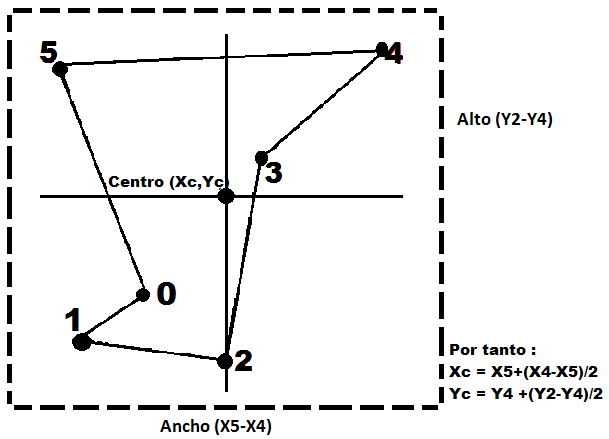
\includegraphics[width=0.95\textwidth]{MetodoRectanguloAureo/Imagenes/rectangulo.png}
        \caption{Ejemplo para calcular el centro del plano de búsqueda.}
        \label{fig:rectangulo}
\end{figure}

%\clearpage \newpage
%\begin{lstlisting}[language=JAVA, caption=Algoritmo Base del Método de Cuadrantes, label=lst:codigo11,escapechar=|]
funcion Inicio()
 {
	RutaSolucion{Puntos[n]}
	ArregloCuadrantes{Cuadrantes[Puntos[n]]}
	Limite = n
	Direccion = derecha
	SubcuadranteOrigen = -1
	CuadranteOrigen = -1
	CuadranteDestino = -1
	Comprobar()
}
funcion Comprobar()
{
	 While (ArregloCuadrantes.length > 0)
	 {
		CuadrantesActual = ArregloCuadrantes[0]
		l = 0
		While CuadrantesActual.length < l {
			PuntosActual = CuadrantesActual[l]
			If(PuntosActual.length < Limite)
			{
				Resolver()
			} 
			else 
			{
				Dividir()  
			}
			l++
		} 
		ArregloCuadrantes.remover[0]
	}
	Terminar()
}	
funcion Dividir()
{
	NuevosCuadrantes{Cuadrantes[Puntos[n]],Cuadrantes[Puntos[n]],Cuadrantes[Puntos[n]],Cuadrantes[Puntos[n]]} = Dividir PuntosActual en 4
	Se reordena el orden de los elementos de NuevosCuadrantes de acuerdo al automata de cuadrantes de la figura \ref {fig:automata.png}
		  -Para ello se calculan 2 ejes (X y Y) a partir de los valores que forman los puntos de ese cuadrante, de ahi se establece el centro que es igual a los valores divididos en 2
		  - A partir de ahi se establece el orden de cuadrantes que va a recorrer para completar la ruta basandose en
				-SubcuadranteOrigen: El cuadrante donde se encuentra
				-En caso de que el cuadrante pertenezca a uno mas grande, el cuadrante al que planea dirigirse el cuadrante padre
					-En caso de no ser menor a 0 significa que planea regresar a si mismo, por tanto puede viajar a direccion, izquierda,derecha,arriba o abajo (por preferencia se eligio izquierda), en el automata de la figura |\ref {fig:automata.png}| se interpretara como estado |$\lambda$|                    
				-En caso de que el cuadrante pertenezca a uno mas grande, el numero de cuadrante padre al que pertenece
					-En caso de no ser menor a 0 significa que planea regresar a si mismo, por tanto puede viajar a dirección, izquierda,derecha,arriba o abajo (por preferencia se eligio izquierda), en el automata de la figura |\ref {fig:automata.png}| se interpretara como estado |$\lambda$|       
	Agregar NuevosCuadrantes a ArregloCuadrantes reemplazando PuntosActual en el mismo lugar donde estaban
	Comprobar()	
}
funcion Resolver()
{
	PuntosActual = Reordenar orden de los elementos de PuntosActual usando metodo de Fuerza Bruta probando todas las combinaciones posibles y obtener el mejor resultado
	agregar PuntosActual a RutaSolucion
	Comprobar()
}
function Terminar()
{
	Mostrar resultados de RutaSolucion
}	
\end{lstlisting}   

\hspace*{1cm} El siguiente paso es definir el criterio que se aplica para saber en qué orden de subcuadrantes debe viajar para recorrer toda la sección.

\subsection{Aplicación de autómatas para el orden de los cuadrantes} 

Para determinar el orden de los cuadrantes por recorrer se utilizará un autómata que recibirá ciertos parámetros y devolverá una de varias soluciones predeterminadas. Los 3 parámetros del autómata son:
    \begin{itemize}
        \item El cuadrante origen: El cuadrante donde se encuentra el cursor.
        \item El cuadrante destino: El cuadrante a donde se dirigirá el cursor.
        \item El origen del subcuadrante: El subcuadrante del cuadrante origen de donde inicia la ruta.
    \end{itemize}
     \begin{figure}[hbtp]
        \centering
            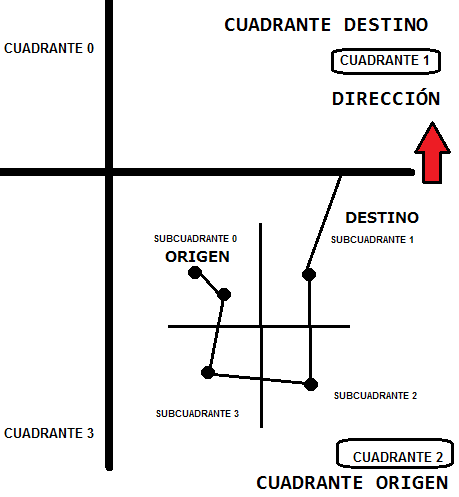
\includegraphics[width=0.6\textwidth]{MetodoRectanguloAureo/Imagenes/findpriori.png}
            \caption{Fragmento de ejemplo del método de cuadrantes.}
            \label{fig:findpriori.png}
    \end{figure}
\hspace*{1cm} En la figura \ref {fig:findpriori.png} se puede observar el fragmento de un ejemplo donde se presentan los cuadrantes 1 y 2; dentro del cuadrante 2 se puede observar que también está dividido en otros subcuadrantes y el punto de origen se encuentra en el subcuadrante 0; de esta forma se obtienen los parámetros necesarios donde:
    \begin{itemize}
        \item El cuadrante origen es 2.
        \item El cuadrante destino es 1.
        \item El origen del subcuadrante es 0.
    \end{itemize}
\hspace*{1cm} Lo primero a notar es que el cursor tendrá que viajar hacia arriba recorriendo los 4 cuadrantes sin pasar por el anterior ya que el cuadrante destino está sobre el cuadrante origen. Para ello se hará uso de una matriz de direcciones presentada en la figura \ref {fig:automatchart.png}.\\

     \begin{figure}[hbtp]
        \centering
            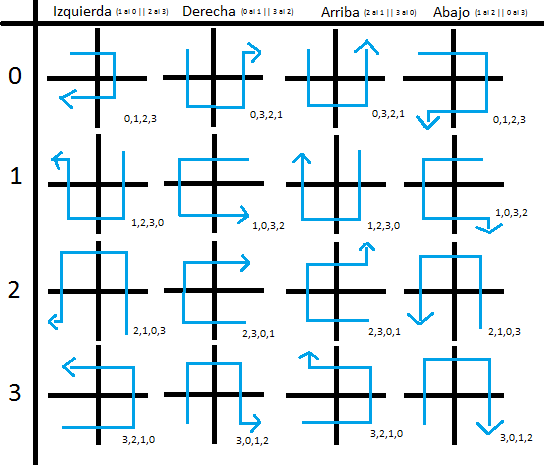
\includegraphics[width=0.8\textwidth]{MetodoRectanguloAureo/Imagenes/automatchart.png}
            \caption{Matriz de direcciones.}
            \label{fig:automatchart.png}
    \end{figure}
    
\hspace*{1cm} Como se puede ver en la figura \ref {fig:automatchart.png} ésta es una matriz de 4 filas y 4 columnas, las filas representan el origen del subcuadrante en donde se va a empezar  (en este caso 0) y las columnas representan la dirección a la que tiene que ir (en este caso hacia arriba y del cuadrante 2 al 1), al tener estas 2 coordenadas se determina como solución la secuencia (0,3,2,1) que determina el orden de subcuadrantes por los que tiene que viajar para pasar por todos los puntos. Cada subcuadrante puede seguir dividiéndose, para tal caso el subcuadrante del origen es siempre el que se está resolviendo al momento, el cuadrante origen y cuadrante destino forman parte del cuadrante anterior.\\
\hspace*{1cm} La primera vez que se vaya a dividir el conjunto de puntos, el parámetro de destino será el mismo punto de origen por tanto; ya teniendo los otros 2 parámetros se puede tomar la solución de cualquiera de las 4 columnas, dando 4 posibles soluciones dependiendo del giro principal. En la figura \ref {fig:example.png} se podrá ver un ejemplo completo aplicando todas las reglas mencionadas.\\

     \begin{figure}[hbt]
        \centering
            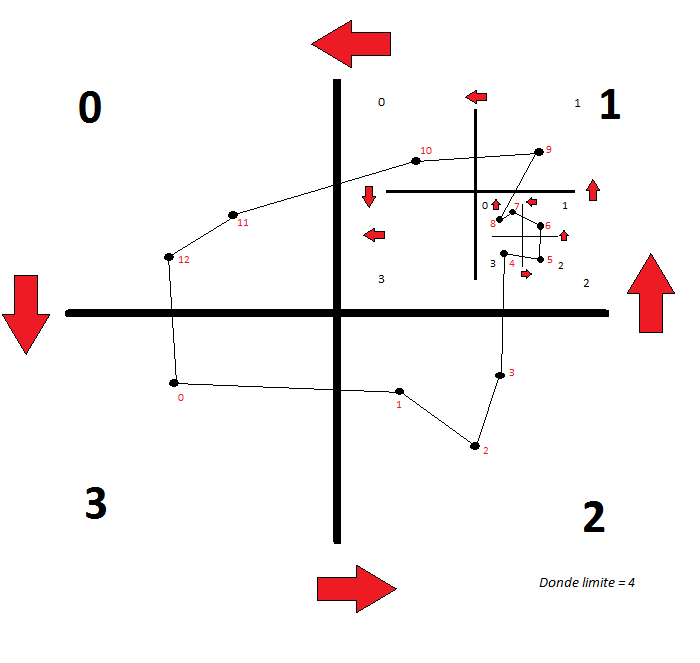
\includegraphics[width=0.7\textwidth]{MetodoRectanguloAureo/Imagenes/example.png}
            \caption{Ejemplo completo de un problema TSP aplicando las reglas mencionadas.}
            \label{fig:example.png}
    \end{figure}
    
\subsubsection{Descripción del autómata}    

En la figura \ref {fig:automata.png} se puede ver el autómata que recibe los 3 parámetros (el cuadrante inicial, el cuadrante donde se tiene que dirigir, y por último el origen del subcuadrante). En la tabla \ref{table:DeclaracionAutomata} se podrá ver su declaración formal.\\

    \begin{figure}[hbtp]
        \centering
            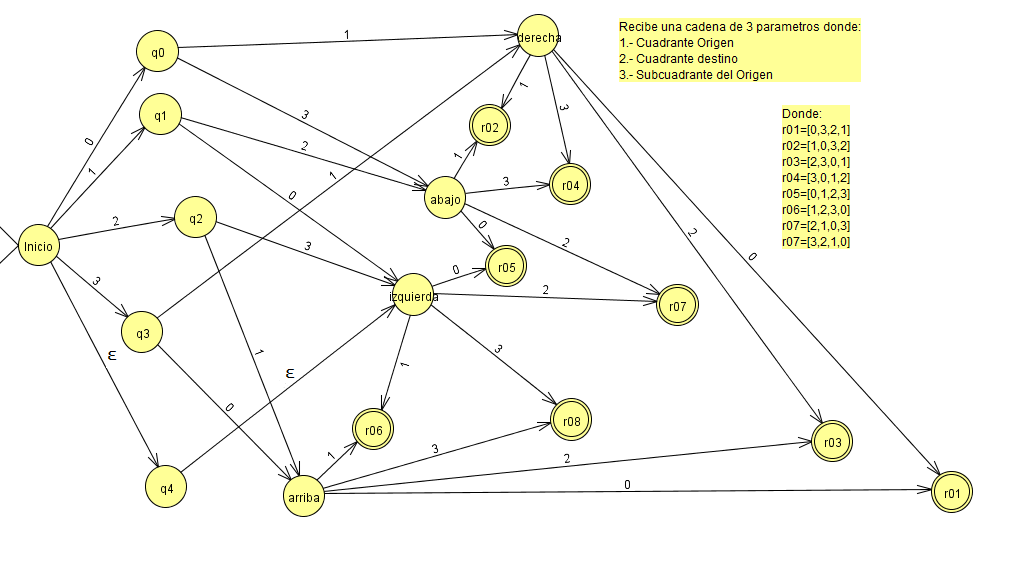
\includegraphics[width=1\textwidth]{MetodoRectanguloAureo/Imagenes/automata2_b.png}
            \caption{Autómata del método de cuadrantes.}
            \label{fig:automata.png}
    \end{figure}    

    \begin{table}[hbtp]
		\centering
		   \caption{Elementos del autómata del método de cuadrantes.}		
		   \begin{tabular}{ | l | l |}
		   \hline
			\rowcolor[gray]{0.5}
			 \hline\multicolumn{2}{|c|}{ \rowcolor[gray]{0.5}Declaración formal} \\\hline
		   \textbf{$\Sigma$}:  & 0, 1, 2, 3      \\ \hline
				 \textbf{$Q$}: & Inicio, q0, q1, q2, q3,q4\\   
							   & izquierda, derecha, arriba, abajo,\\ 
							   & r01, r02, r03, r04, r05, r06, r07, r08     \\ \hline
				\textbf{$q0$}: & Inicio     \\ \hline
				\textbf{$F$}:  & r01, r02, r03, r04, r05, r06, r07, r08     \\ \hline
			\textbf{$\delta$}: & Es la relación de transiciones que se muestran en la tabla \ref{table:Automata}. \\ \hline
		   \end{tabular}
		   \label{table:DeclaracionAutomata}
       \end{table}
       
\hspace*{1cm} Como se puede ver en la tabla \ref{table:Automata}, la transición de eventos que realiza el autómata es del tipo no determinista ya que posee estados vacíos y transiciones $\epsilon$.

	 \begin{table}[hbtp]
		 \centering
			\caption{Transiciones del autómata del método de cuadrantes.}		 
			\begin{tabular}{ | l | l | l | l | l | l |}
			\hline
			  \rowcolor[gray]{0.5}
				   & 0         & 1       & 2       & 3         &$\epsilon$   \\ \hline
			Inicio & q0        & q1      & q2      & q3        & q4         \\ \hline      
				q0 &           & derecha &         & abajo     &            \\ \hline
				q1 & izquierda &         & abajo   &           &            \\ \hline
				q2 &           & arriba  &         & izquierda &            \\ \hline
				q3 & arriba    &         & derecha &           &            \\ \hline
				q4 &           &         &         &           & izquierda  \\ \hline
		 izquierda & r05       & r06     & r07     & r08       &            \\ \hline
		   derecha & r01       & r02     & r03     & r04       &            \\ \hline
			arriba & r01       & r06     & r03     & r08       &            \\ \hline
			 abajo & r05       & r02     & r07     & r04       &            \\ \hline
			  *r01 &           &         &         &           &            \\ \hline
			  *r02 &           &         &         &           &            \\ \hline
			  *r03 &           &         &         &           &            \\ \hline
			  *r04 &           &         &         &           &            \\ \hline
			  *r05 &           &         &         &           &            \\ \hline
			  *r06 &           &         &         &           &            \\ \hline
			  *r07 &           &         &         &           &            \\ \hline
			  *r08 &           &         &         &           &            \\ \hline
			\end{tabular}
			\label{table:Automata}
	\end{table}
    

    
\hspace*{1cm} En el ejemplo a la figura \ref {fig:example.png} el cuadrante 1 está dividido en otros subcuadrantes, el origen del subcuadrante sería el punto el 4 que se encuentra en el cuadrante 2, ya que a la dirección por la que va tiene que ir al cuadrante principal 0. Por tanto, los parámetros que recibiría el autómata en ese mismo orden sería: 

\begin{itemize}
\item El cuadrante origen: El cuadrante 1.
\item El cuadrante destino:El cuadrante 0 que se encuentra a su izquierda.
\item El origen del subcuadrante: El subcuadrante 2.
\end{itemize}

\hspace*{1cm}Como se observa en la figura \ref {fig:automata.png}, primero se recorrería al estado $q2$, luego pasaría por el estado $izquierda$ y por último al estado $r7$, dando como resultado los parámetros (2,1,0,3) que vendrían siendo los cuadrantes por recorrer en la iteración inicial. Sin embargo el subcuadrante 1 excede con el límite de puntos establecido teniendo que resolver primero este inconveniente repitiendo el proceso de subdivisión esta vez poniendo el origen, destino y subcuadrante del origen como 2, 1 y 3 respectivamente, lo que daría el estado $r8$ con los parámetros (3,2,1,0).\\
\hspace*{1cm} De ahí en adelante se resuelven los demás cuadrantes usando el método de fuerza bruta, que gracias a las divisiones que se fueron haciendo agilizan el proceso, terminando mucho más rápido que haber intentado hacer el método de fuerza bruta con todos los puntos.\\

\subsection{Comentarios finales}
Este método hace uso del sentido común y de la distribución uniforme para cumplir con el objetivo deseado, no se busca obtener todavía un resultado definitivo, sino una buena solución que servirá de base para la aplicación de las metaheurísticas correspondientes.\\
\hspace*{1cm} El uso de cuadrantes permite seccionar por zonas de manera finita y no salir de cada una de ellas hasta pasar por todos los lugares, reduciendo el tiempo de cálculo y evitando realizar combinaciones innecesarias.\\ 
\hspace*{1cm} Sin embargo y a pesar de obtener una buena solución, el resultado obtenido a través de este algoritmo no es la mejor ruta que se haya creado hasta la fecha, sino es una respuesta cercana que se puede refinar aplicando metaheurísticas, tema que se verá en el capítulo 5.\\
\hspace*{1cm} Lo que destaca de este método es la de obtener buenos resultados y la preferencia de recorrer zonas cercanas con tiempos de cálculo breves en lugar de intentar hacer movimientos audaces o combinaciones reiterativas que pueden ser solo una pérdida de tiempo, aunque eso también implica una desventaja ya que jamás podría obtener resultados mejores a costa de mayor trabajo.\\
\hspace*{1cm} Como se muestra en la figura \ref {fig:monalisatsp2.png}, es un retrato de la Mona Lisa hecho a base de un problema de TSPLIB obtenido de \cite{[MONALISA]}, usando el algoritmo de cuadrantes se pudo unir los puntos que componían el problema mostrando la figura presentada.
    \begin{figure}[hbtp]
        \centering
            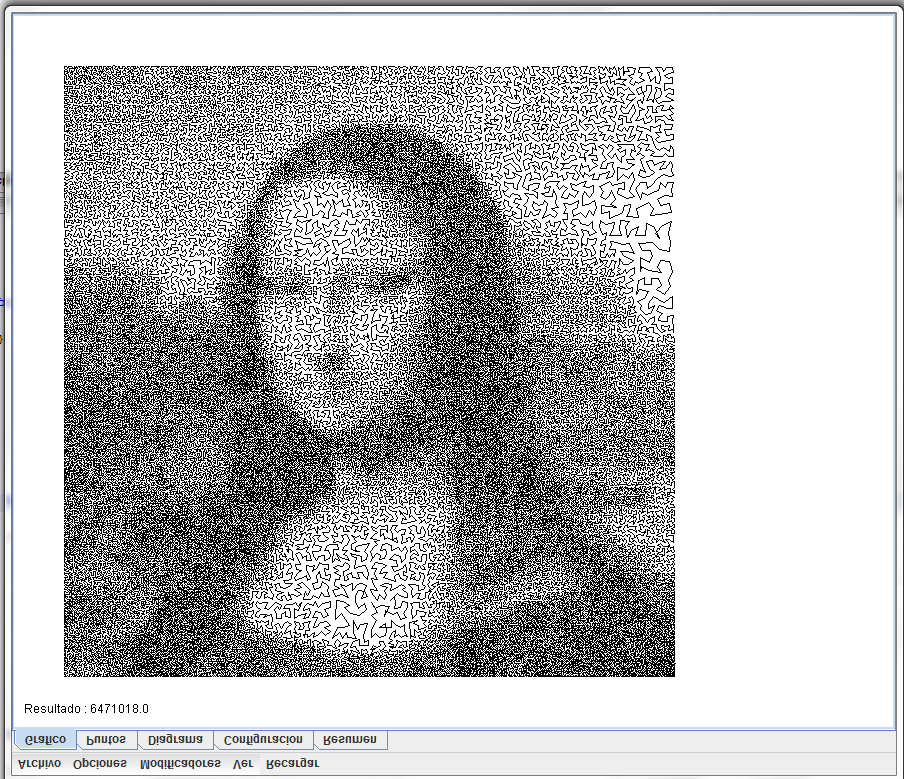
\includegraphics[width=0.9\textwidth]{MetodoRectanguloAureo/Imagenes/monalisatsp.png}
            \caption{Ejemplo de ejercicio de la MonaLisa hecha en TSP.}
            \label{fig:monalisatsp2.png}
    \end{figure} 
        \chapter{}
    \vspace*{10cm}
    \begin{center}
        %\thispagestyle{empty} 
        \section*{ CAPÍTULO 4 : Documentación del software usado en las pruebas }
        \addcontentsline{toc}{section}{CAPÍTULO 4 : Documentación del software usado en las pruebas }
        \addtocounter{section}{1}
        \setcounter{subsection}{0}
        \setcounter{figure}{0}
        \setcounter{lstlisting}{0}
        \setcounter{table}{0} 
    \end{center}

    \clearpage \newpage
    \vspace*{8cm}
    \subsection{Introducción}
 Para poder aplicar el algoritmo propuesto con las instancias obtenidas de la TSPLIB, se desarrolló un programa utilizando el lenguaje de programación JAVA que permita almacenar datos en diferentes formatos (XML, JSON,TSPLIB).\\
 \hspace*{1cm}Otro propósito de este programa es que sea de código abierto con el fin de que otras personas puedan continuar con la investigación o utilizarlo como referencia para otros proyectos. Una vez que se explique la composición del software y la forma en la que se utiliza en el siguiente capítulo se procederá al desarrollo de los experimentos.\\
 
\subsection{Componentes} 
En la figura \ref {fig:Software_1} se muestra la ventana principal del programa que está compuesto por:
    \begin{enumerate}[label=\Alph*.-]
    \item Una barra de herramientas
    \item 3 pestañas cuyo contenido se explicará a continuación
    \item La pantalla principal que muestra un problema de TSP
    \end{enumerate}
\hspace*{1cm}Como se observa en la figura \ref {fig:Software_1} la ventana muestra la posición de los puntos del problema y las rutas que éste recorrió de principio a fin; también se muestran los cuadrantes que se trazaron para realizar el cálculo así como el orden de puntos en que se fue recorriendo.\\ 
     \begin{figure}[hbtp]
        \centering
            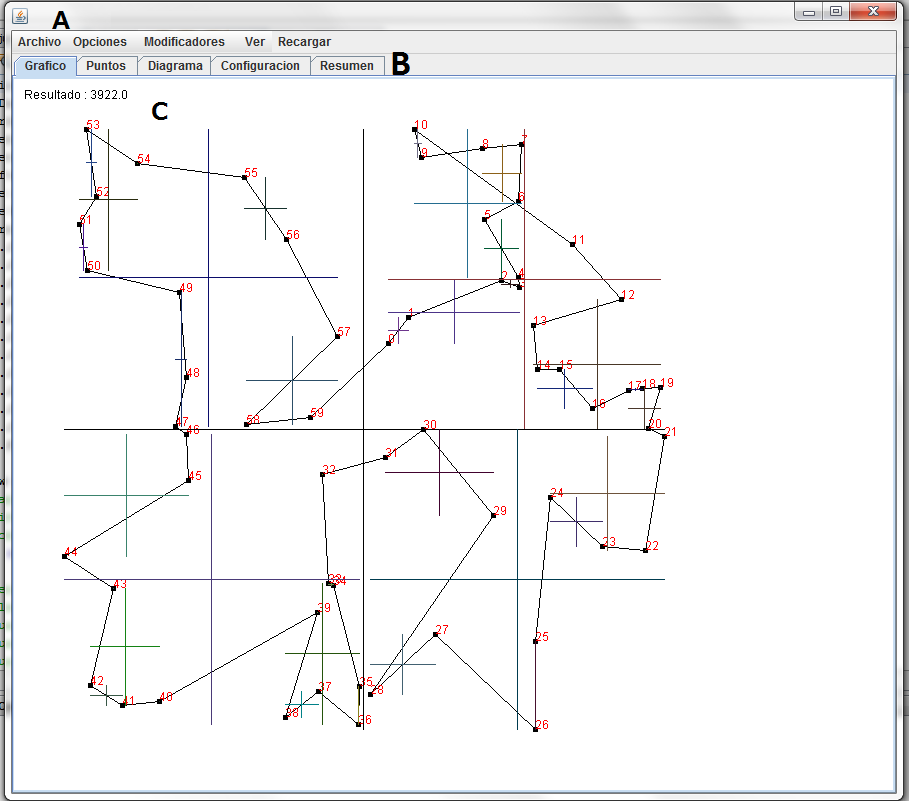
\includegraphics[width=1\textwidth]{Software/Imagenes/Software_1.png}
            \caption{Descripción de la ventana principal del software.}
            \label{fig:Software_1}
    \end{figure}

\hspace*{1cm}En la figura \ref {fig:Software_2} se muestran las coordenadas de los puntos del problema junto con el resultado mostrado en la figura \ref {fig:Software_1}.\\
     \begin{figure}[hbtp]
        \centering
            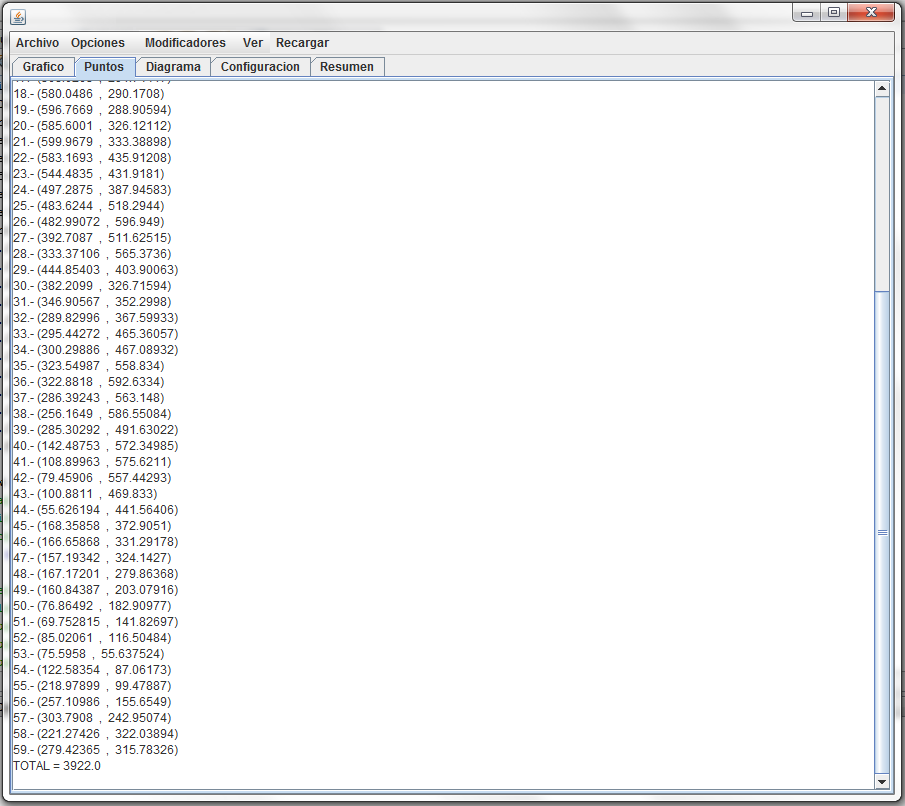
\includegraphics[width=0.4\textwidth]{Software/Imagenes/Software_2.png}
            \caption{Coordenadas de los puntos del problema.}
            \label{fig:Software_2}
    \end{figure}
    
\hspace*{1cm}En la figura \ref {fig:Software_3} se muestra la gráfica de los resultados obtenidos en el problema utilizando diferentes metaheurísticas. En este ejemplo se aplicó únicamente el algoritmo de recocido simulado.\\
     \begin{figure}[hbtp]
        \centering
            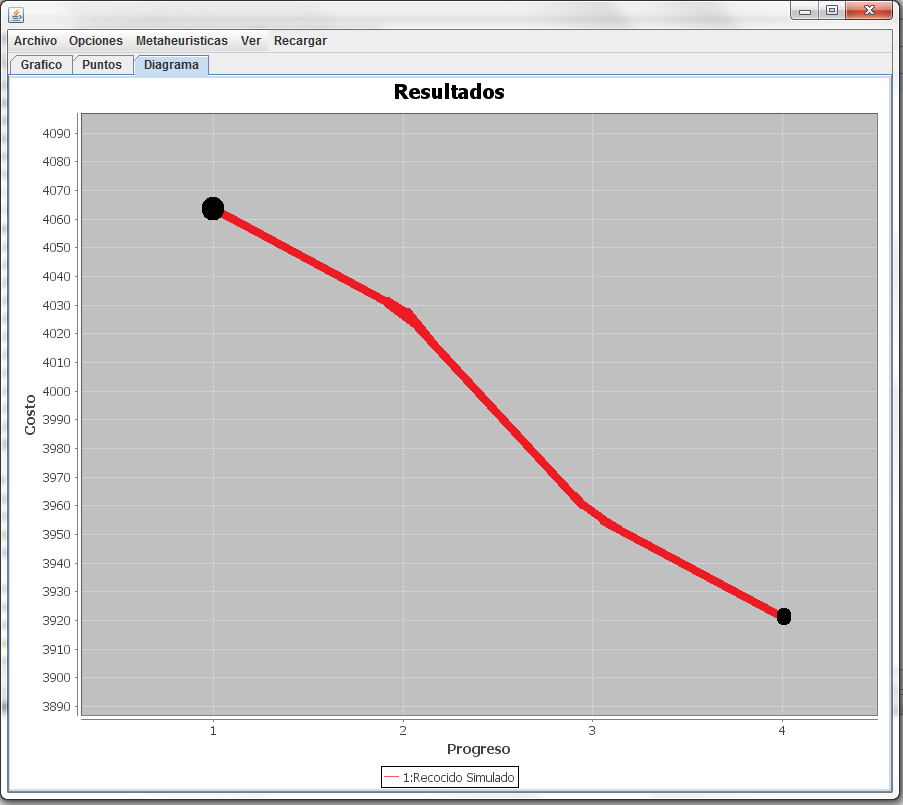
\includegraphics[width=0.4\textwidth]{Software/Imagenes/Software_3.png}
            \caption{Gráfica de los resultados del problema.}
            \label{fig:Software_3}
    \end{figure}
  
\hspace*{1cm}En la figura \ref {fig:Software_9} se muestra la ventana de configuraciones que se puede realizar para cada metaheurística, como la cantidad de ciclos que se puede hacer, el tamaño de los genes, factor de temperatura para el proceso de recocido simulado, etc. El uso de estas variables se explicarán en el siguiente capítulo.\\
     \begin{figure}[hbtp]
        \centering
            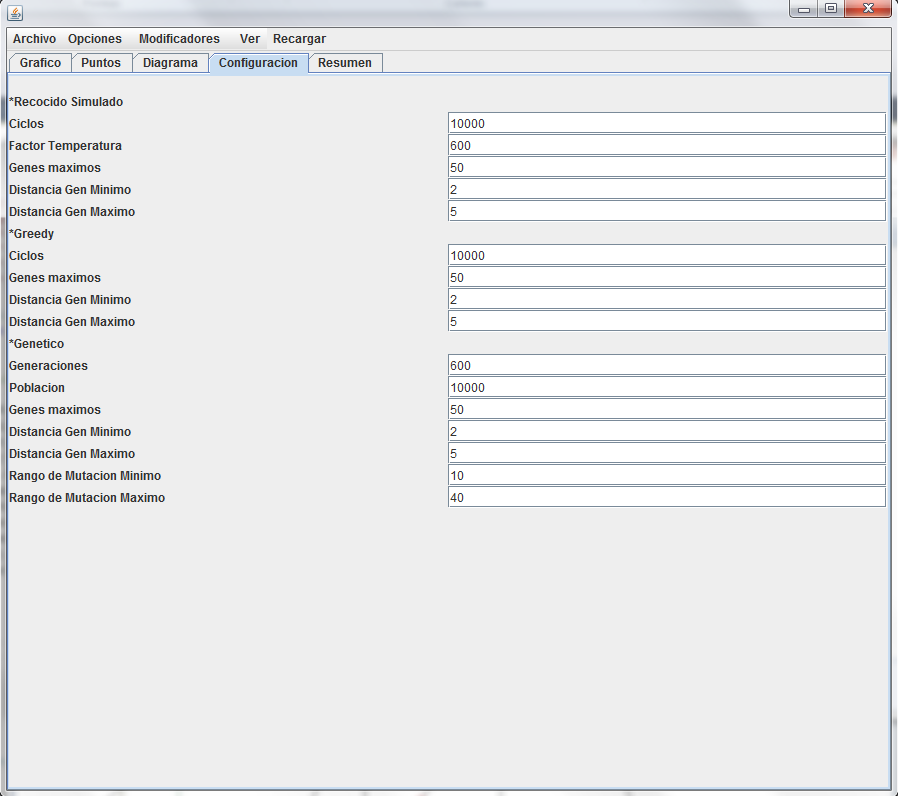
\includegraphics[width=0.6\textwidth]{Software/Imagenes/Software_9.png}
            \caption{Ventana de configuración.}
            \label{fig:Software_9}
    \end{figure}
    
\hspace*{1cm}En la figura \ref {fig:Software_10} se muestra una pantalla que despliega la cantidad de tiempo que tarda el algoritmo cada vez que se ejecuta un problema.\\
     \begin{figure}[hbtp]
        \centering
            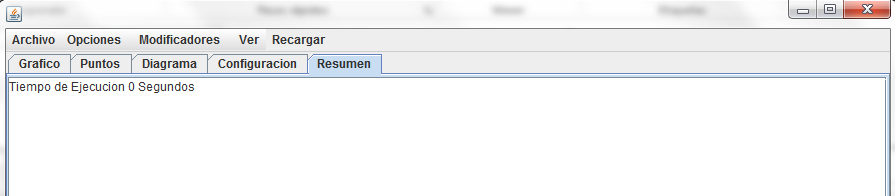
\includegraphics[width=0.7\textwidth]{Software/Imagenes/Software_10.png}
            \caption{Ventana de resultados.}
            \label{fig:Software_10}
    \end{figure}
    
\hspace*{1cm}En la figura \ref {fig:Software_4} se puede observar el menú de Archivo de la barra de herramientas, que tiene las siguientes opciones:

\begin{enumerate}[label=\Alph*.-]
\item \textbf{Guardar:} Permite guardar las coordenadas para poder usarse en experimentos futuros en un archivo .TSP.
\item \textbf{Abrir:} Abre un documento .TSPLIB o .TXT y carga sus coordenadas en el programa, una vez que se carguen los datos el problema se resolverá automáticamente.
\item \textbf{Abrir sin resolver:}Lo mismo que el botón anterior, solo que no resuelve el problema de forma automática.
\item \textbf{Abrir Prueba:} Permite abrir un archivo XML ó JSON y cargar un problema con sus respectivos resultados. Estos problemas se consiguen a través de los siguientes botones.
\item \textbf{Guardar (XML):} Permite guardar un problema con todos los resultados obtenidos en un archivo XML.
\item \textbf{Guardar (JSON):} Lo mismo que el anterior, pero lo guarda en formato JSON.
\item \textbf{Realizar Experimento:} Este será la función que se usará para realizar las actividades del siguiente capítulo, permite realizar de manera consecutiva una serie de ejecuciones del mismo listado de puntos que se encuentra cargados, guardando los resultados de forma física con el archivo .JSON de cada resultado y su gráfica correspondiente. Por ejemplo si se seleccionan 30 ejecuciones devolverá 30 archivos .json y 30 gráficas de cada uno.
\end{enumerate}

     \begin{figure}[hbtp]
        \centering
            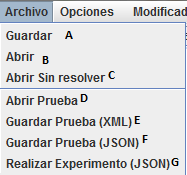
\includegraphics{Software/Imagenes/Software_4.png}
            \caption{Barra de herramientas, Archivo.}
            \label{fig:Software_4}
    \end{figure}
    
\hspace*{1cm}En la figura \ref {fig:Software_5} se muestra el menú de Opciones, la cual contiene funciones de diversos propósitos:
\begin{enumerate}[label=\Alph*.-]
\item  \textbf{Aleatorio:} Permite generar una serie de coordenadas al azar y que resolverá de manera automática, el propósito original de esta función fue la de probar el algoritmo de búsqueda por cuadrantes conforme se fue desarrollando.
\item  \textbf{Borrar resumen:} Permite limpiar la pantalla de la ventana de resumen de la figura \ref {fig:Software_10}.
\end{enumerate}
     \begin{figure}[hbtp]
        \centering
            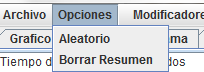
\includegraphics{Software/Imagenes/Software_5.png}
            \caption{Barra de herramientas, Opciones.}
            \label{fig:Software_5}
    \end{figure}

\hspace*{1cm}En la figura \ref {fig:Software_6} se puede observar el menú de modificadores que se encarga de aplicar las perturbaciones de la solución base; éstas se harán al final de la ejecución del método de cuadrantes (si se marcó como seleccionado el método de cuadrantes) con el fin de optimizar la solución base, los algoritmos que se pueden seleccionar son:
    
\begin{enumerate}[label=\Alph*.-]
\item Cuadrantes 
\item Búsqueda Exhaustiva
\item Recocido Simulado
\item Búsqueda Greedy
\item Algoritmo Genético
\end{enumerate}

     \begin{figure}[hbtp]
        \centering
            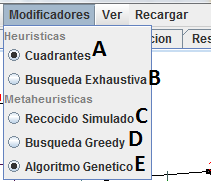
\includegraphics[width=0.3\textwidth]{Software/Imagenes/Software_6.png}
            \caption{Barra de herramientas, Modificadores.}
            \label{fig:Software_6}
    \end{figure}
    
\hspace*{1cm}En la figura \ref {fig:Software_7} se puede observar el menú de Ver, que permite dibujar el diagrama de la figura \ref {fig:Software_1} de acuerdo a los elementos que aparecen en el listado:

\begin{enumerate}[label=\Alph*.-]
\item \textbf{Ruta:} Las líneas que muestra el recorrido de punto a punto.
\item \textbf{Puntos:}Los nodos que indican la ubicación exacta de cada punto.
\item \textbf{Lineas:} Las divisiones de colores que los cuadrantes de acuerdo al método de cuadrantes.
\item \textbf{Números:} El orden de los puntos que recorrió la ruta de principio a fin.
\item \textbf{Final:} La última ruta que se recorre del último punto hacia el punto de inicio.
\end{enumerate}

     \begin{figure}[hbtp]
        \centering
            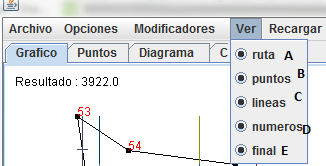
\includegraphics[width=0.7\textwidth]{Software/Imagenes/Software_7.png}
            \caption{Barra de herramientas, Ver.}
            \label{fig:Software_7}
    \end{figure}
    
\hspace*{1cm}En la figura \ref {fig:Software_8} se puede observar la opción de Recargar que permite volver a generar el problema; la utilidad de esta función es la de reutilizar el mismo problema usando los diferentes métodos de la figura \ref {fig:Software_6} o bien, esperar obtener resultados diferentes.\\

     \begin{figure}[hbtp]
        \centering
            
\includegraphics{Software/Imagenes/Software_8.png}
            \caption{Barra de herramientas, Recargar.}
            \label{fig:Software_8}
    \end{figure}
    
\subsection{Uso del software}
Ya conociendo los componentes que conforman el programa se procederá a explicar la manera en que se usará para los experimentos.\\
\hspace*{1cm}Al iniciar el programa se mostrará una ventana parecida a la de la figura \ref {fig:Software_1} donde se muestra un problema formado por un conjunto de puntos al azar ya resuelto, sin embargo para esta ocasión se usará un archivo .TSP como prueba. Primero se usará la opción de Abrir sin resolver como se muestra en la figura \ref {fig:Software_Uso_1}.
     \begin{figure}[hbtp]
        \centering
            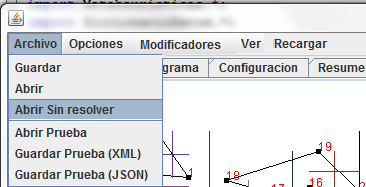
\includegraphics[width=0.5\textwidth]{Software/Imagenes/Software_Uso_1.png}
            \caption{Abrir sin resolver.}
            \label{fig:Software_Uso_1}
    \end{figure}
    
\hspace*{1cm}Para este ejemplo se usará el archivo 'ch150.tsp' como se muestra en la figura \ref {fig:Software_Uso_2}, la mejor ruta conocida para este problema es de 6528 unidades. 
     \begin{figure}[hbtp]
        \centering
            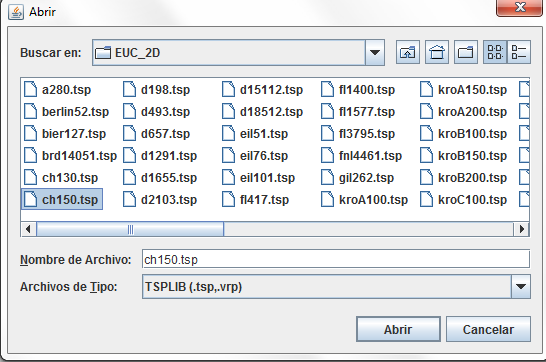
\includegraphics[width=0.55\textwidth]{Software/Imagenes/Software_Uso_2.png}
            \caption{Archivo .TSP.}
            \label{fig:Software_Uso_2}
    \end{figure}
    
\hspace*{1cm}En la figura \ref {fig:Software_Uso_3} se puede apreciar que los puntos se encuentran desordenados, por tanto genera una ruta de lo más ineficiente con un costo de 52890 unidades ya que uno los puntos en el mismo orden que los va leyendo.\\

    \begin{figure}[hbtp]
        \centering
            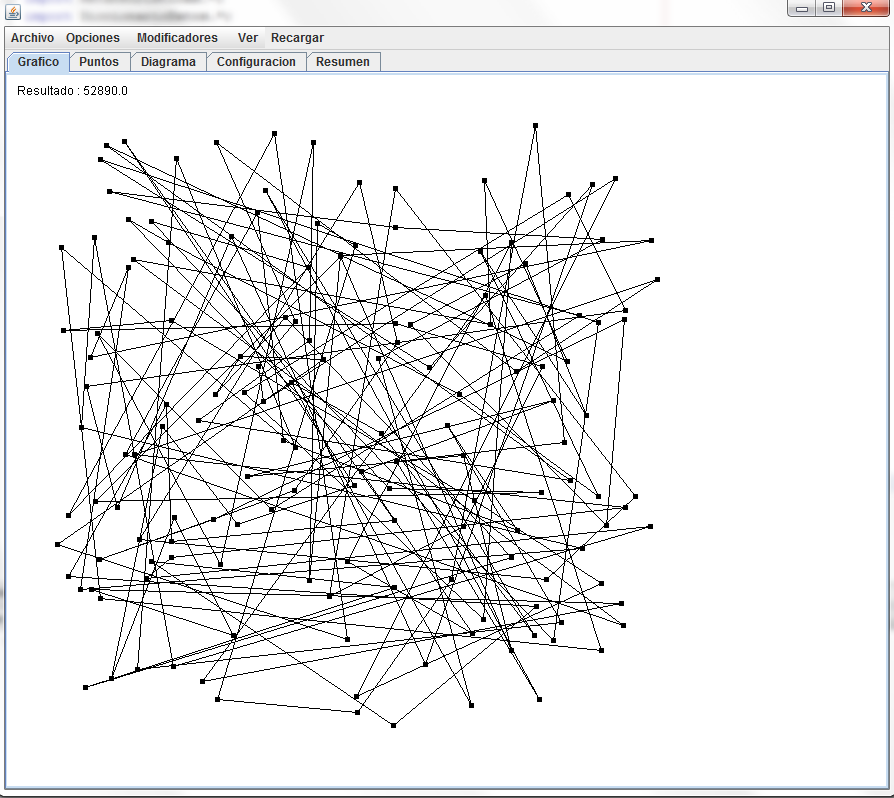
\includegraphics[width=0.9\textwidth]{Software/Imagenes/Software_Uso_3.png}
            \caption{Archivo sin resolver.}
            \label{fig:Software_Uso_3}
    \end{figure}

\clearpage \newpage

\hspace*{1cm}Sin embargo si se aplica la opción de recargar se aplicará las fórmulas que se tienen seleccionadas, en este caso solo se aplicará el método de cuadrantes, tal como se muestra en la figura \ref {fig:Software_Uso_4}. Los puntos siguen siendo los mismos pero el trazado de rutas está ordenado de acuerdo dicho método trayendo un costo de 8579 unidades, siendo menos de una sexta parte del costo de la figura \ref {fig:Software_Uso_3}.\\

    \begin{figure}[hbtp]
        \centering
            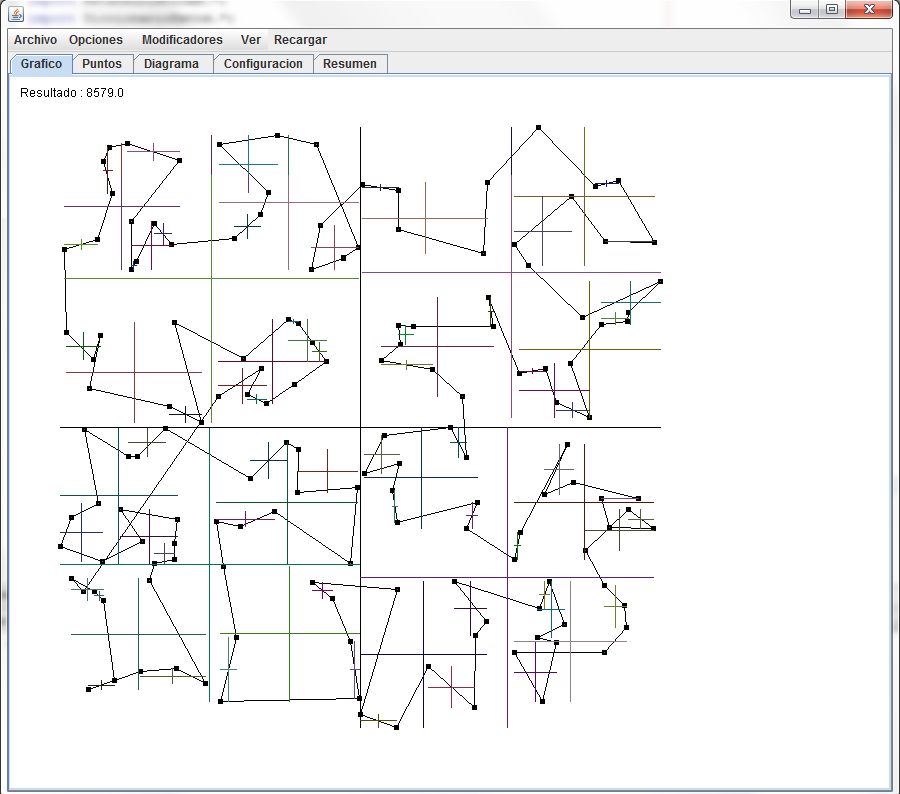
\includegraphics[width=0.9\textwidth]{Software/Imagenes/Software_Uso_4.png}
            \caption{Problema resuelto con el método de cuadrantes.}
            \label{fig:Software_Uso_4}
    \end{figure}
\clearpage \newpage

\hspace*{1cm}En la figura \ref {fig:Software_Uso_5} se volvió a recargar el mismo problema pero esta vez usando el método de búsqueda exhaustiva la cual trae un valor de 8252 unidades, un valor ligeramente menor al anterior con 327 unidades de diferencia.\\

    \begin{figure}[hbtp]
        \centering
            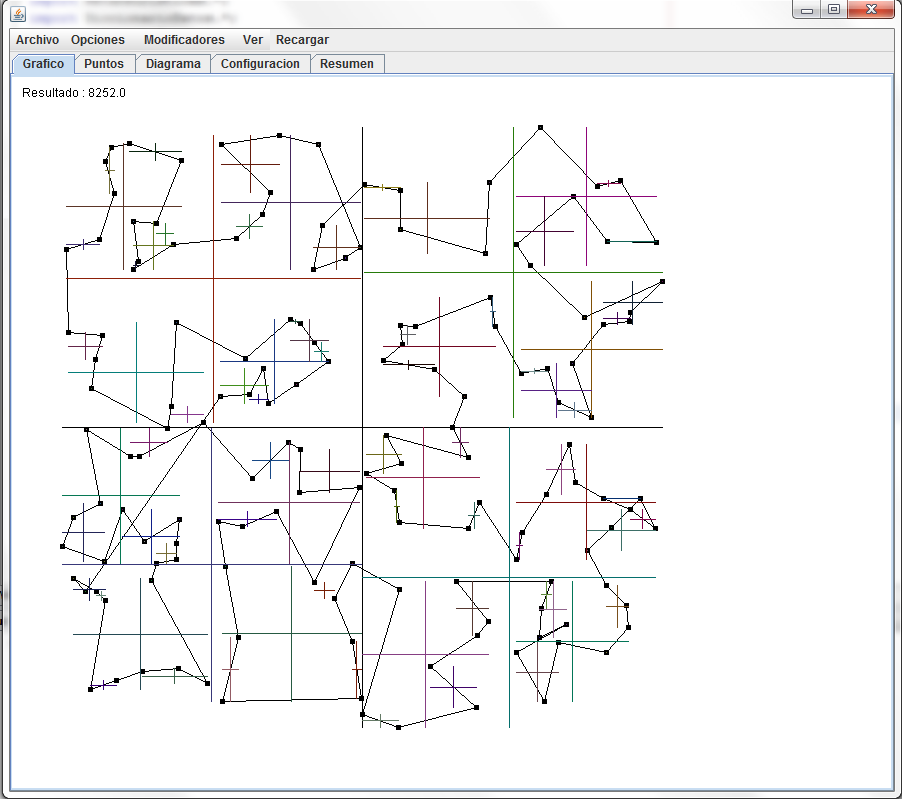
\includegraphics[width=0.9\textwidth]{Software/Imagenes/Software_Uso_5.png}
            \caption{Problema resuelto con el método de cuadrantes y la búsqueda exhaustiva en el orden correspondiente.}
            \label{fig:Software_Uso_5}
    \end{figure}
\clearpage \newpage

\hspace*{1cm}En la figura \ref {fig:Software_Uso_6} se volvió a recargar el mismo problema pero esta vez marcando también el método de recocido simulado con un resultado de 8179 unidades, una mejora de la figura \ref {fig:Software_Uso_5} con 73 unidades de diferencia.\\

    \begin{figure}[hbtp]
        \centering
            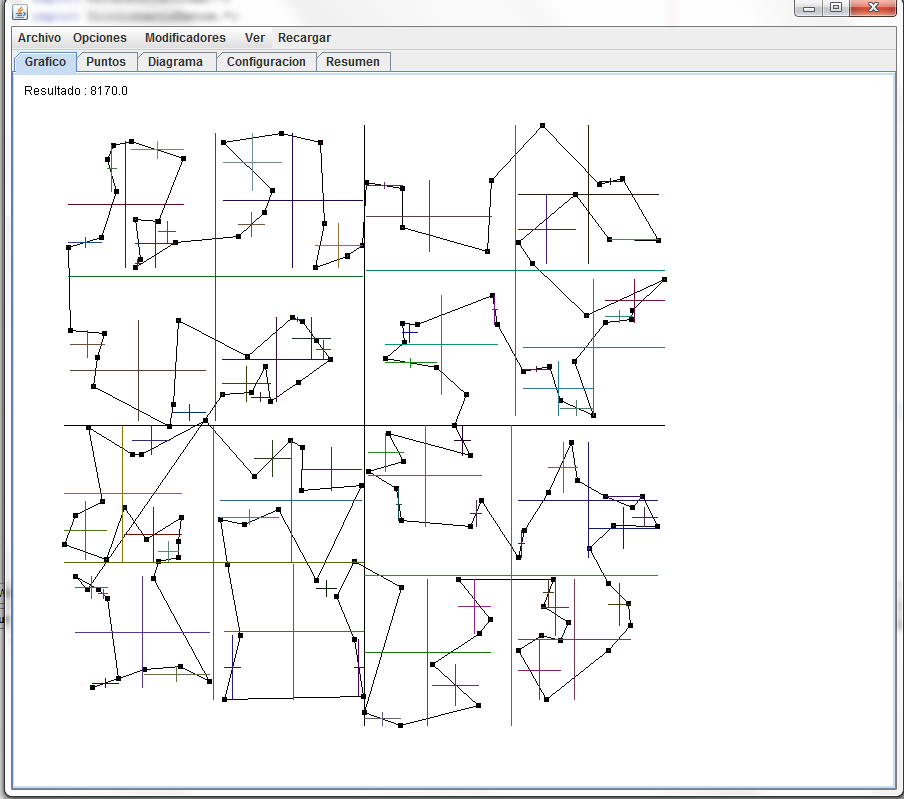
\includegraphics[width=0.9\textwidth]{Software/Imagenes/Software_Uso_6.png}
            \caption{Problema resuelto con el método de cuadrantes, recocido simulado y búsqueda exhaustiva en el orden correspondiente.}
            \label{fig:Software_Uso_6}
    \end{figure}
\clearpage \newpage

\hspace*{1cm}En la figura \ref {fig:Software_Uso_7} se puede mostrar la gráfica de la forma en que fue mejorando la solución obtenida por el programa. El método de Búsqueda exhaustiva siempre se ejecutará al final del proceso.\\

    \begin{figure}[hbtp]
        \centering
            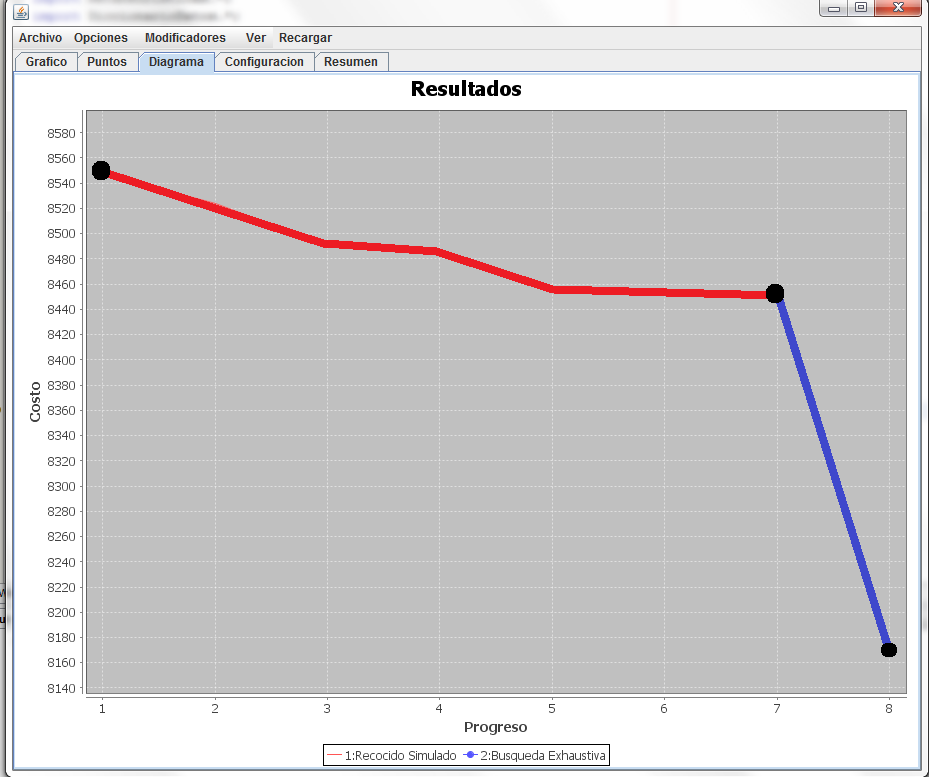
\includegraphics[width=0.9\textwidth]{Software/Imagenes/Software_Uso_7.png}
            \caption{Gráfica que muestra los resultados.}
            \label{fig:Software_Uso_7}
    \end{figure}
\clearpage \newpage

\hspace*{1cm}Por último, aplicando el algoritmo genético en la figura \ref {fig:Software_Uso_8} con el fin de obtener el mejor resultado posible, deja un costo de 7342 unidades con una notable diferencia de 837 unidades.\\

    \begin{figure}[hbtp]
        \centering
            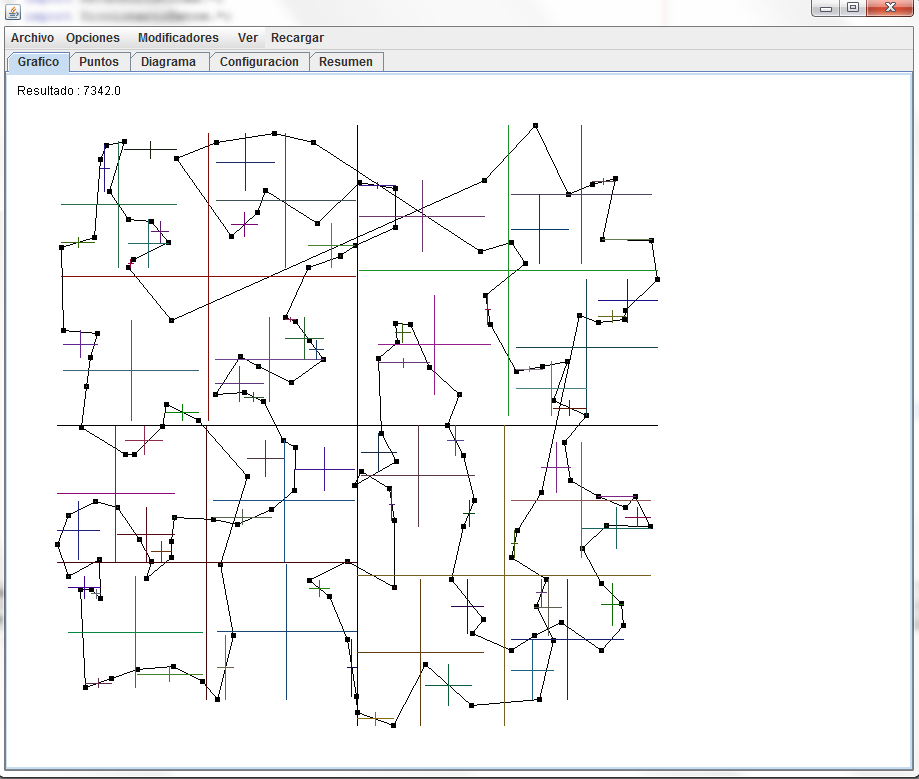
\includegraphics[width=0.9\textwidth]{Software/Imagenes/Software_Uso_8.png}
            \caption{Problema resuelto usando todas las metaheurísticas.}
            \label{fig:Software_Uso_8}
    \end{figure}
\clearpage \newpage

\hspace*{1cm}En la figura \ref {fig:Software_Uso_9}, se puede observar la gráfica con el resultado de la figura \ref {fig:Software_Uso_8} el cual muestra un resultado favorable en la línea que representa el algoritmo genético, debido a su simplicidad el método de búsqueda exhaustiva se aplica al final de las demás metahuerísticas.\\

    \begin{figure}[hbtp]
        \centering
            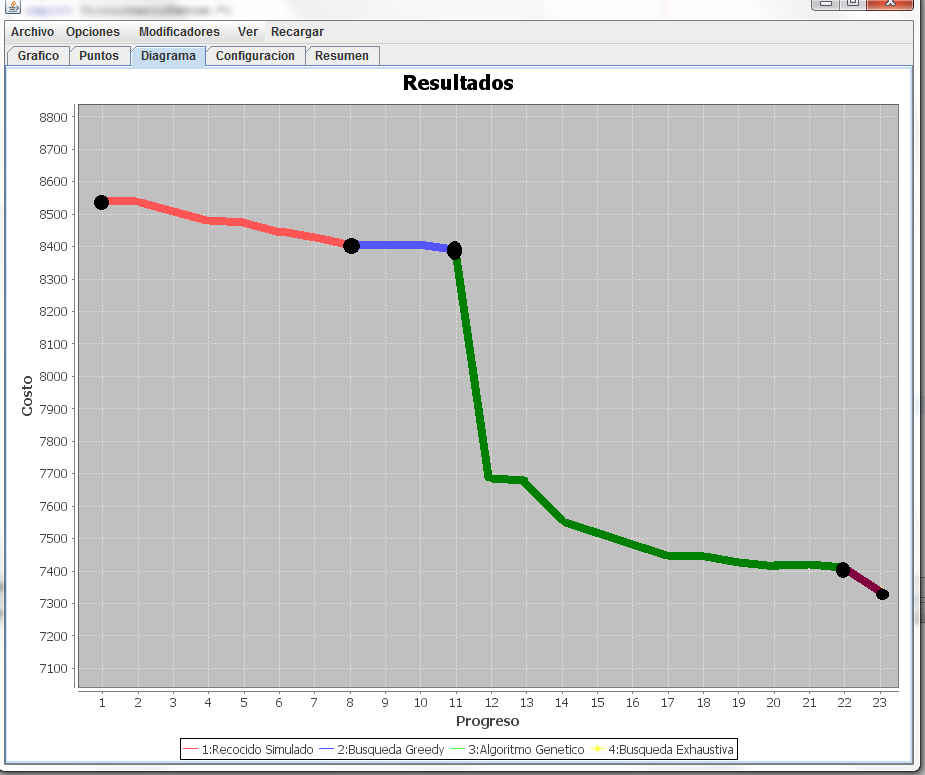
\includegraphics[width=0.9\textwidth]{Software/Imagenes/Software_Uso_9.png}
            \caption{Gráfica que muestra el progreso después de aplicar todas las metahuerísticas.}
            \label{fig:Software_Uso_9}
    \end{figure}  
\clearpage \newpage

\hspace*{1cm}Para finalizar si se desea mostrar el problema resuelto se puede guardar por medio de un archivo .XML o un .JSON descritos en la figura \ref {fig:Software_4}. En la figura \ref {fig:Software_Uso_10} se eligió en formato .JSON.\\
    \begin{figure}[hbtp]
        \centering
            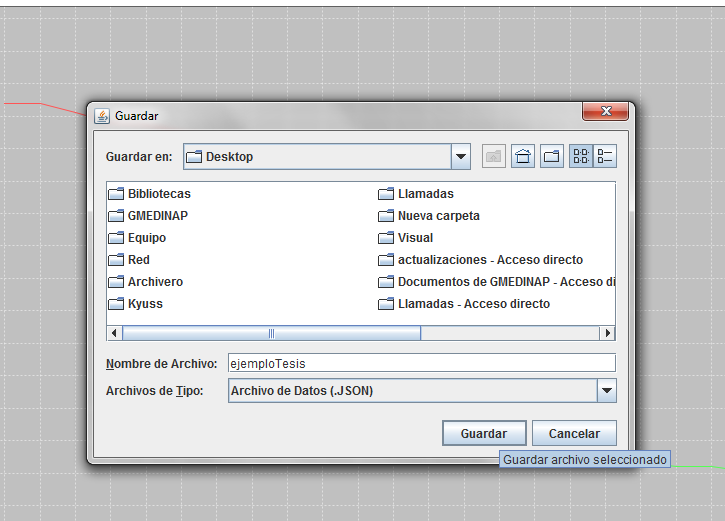
\includegraphics[width=0.5\textwidth]{Software/Imagenes/Software_Uso_10.png}
            \caption{Problema solucionado guardado en un JSON.}
            \label{fig:Software_Uso_10}
    \end{figure}

\subsection{Comentarios finales}
La ayuda de este programa fue esencial para poder realizar los experimentos, ya que gracias a esta herramienta fue posible leer, interpretar y almacenar los resultados correspondientes.\\
\hspace*{1cm}Una de las ventajas de este programa es que sigue el mismo formato de las TSPLIB, por tanto puede utilizarse para otros proyectos futuros, sin embargo solo está limitado a resolver problemas que utilizan distancia euclidiana (EUC2D).\\ 
        \chapter{}
    \vspace*{10cm}
    \begin{center}
        %\thispagestyle{empty} 
        \section*{ CAPÍTULO 5 :  Pruebas y análisis de resultados }
        \addcontentsline{toc}{section}{CAPÍTULO 5 : Pruebas y análisis de resultados}
        \addtocounter{section}{1}
        \setcounter{subsection}{0}
        \setcounter{figure}{0}
        \setcounter{lstlisting}{0}
        \setcounter{table}{0} 
    \end{center}

    \clearpage \newpage
    \vspace*{8cm}
    En este capítulo se aplicará lo expuesto en los capítulos 3 y 4 para realizar los experimentos correspondientes, y se describirán los resultados obtenidos.

\subsection{Introducción}
    
El último capítulo trata sobre el uso de los algoritmos y metaheurísticas aplicados sobre problemas reales de TSP, primero se explicará el proceso que se realizó y al final se mostrarán los resultados obtenidos.\\
\hspace*{1cm}Cada uno de los problemas de TSP se probará tanto con el método de cuadrantes como sin este método; en ambos casos se probará con algo conocido como "mutación" que alterará la solución base reordenando algunos de sus puntos con el fin de obtener resultados aleatorios pero coherentes. Como se muestra en la tabla \ref {table:DescripcionPruebasTSP} estos serán los problemas a utilizar obtenidos en la página de la Universidad de Heidelberg \cite {[TSPLIB]} y cuyas descripciones se obtuvieron de la Universidad de Waterloo \cite{[TSPLIB2]}.

% Please add the following required packages to your document preamble:
% \usepackage[table,xcdraw]{xcolor}
% If you use beamer only pass "xcolor=table" option, i.e. \documentclass[xcolor=table]{beamer}
\begin{table}[]
\centering
\caption{Descripción de los problemas de TSP usados para las pruebas.}
\resizebox{1\textwidth}{!}{
\rotatebox{0}{
\begin{tabular}{lcll}
\hline
\rowcolor[HTML]{9B9B9B} 
\multicolumn{1}{c}{\cellcolor[HTML]{9B9B9B}{\color[HTML]{FFFFFF} \textbf{Problema}}} & {\color[HTML]{FFFFFF} \textbf{Ciudades}} & \multicolumn{1}{c}{\cellcolor[HTML]{9B9B9B}{\color[HTML]{FFFFFF} \textbf{Descripción}}} & \multicolumn{1}{c}{\cellcolor[HTML]{9B9B9B}{\color[HTML]{FFFFFF} \textbf{Autor}}} 	\\ \hline
a280.tsp                                                                             & 280                                      & Problema de perforación						                                   		  & Ludwig                                   		  								  	\\ \hline
brd14051.tsp                                                                         & 14051                                    & Republica federal de Alemania en 1989                                                   & Bachem y Wottawa                                   		  							\\ \hline
ch150.tsp                                                                            & 150                                      & Problema de 150 ciudades							                                      & Churritz                                   		  									\\ \hline
d1655.tsp                                                                            & 1655                                     & Problema de perforación						                                          & Reinelt                                   		  									\\ \hline
d493.tsp                                                                             & 493                                      & Problema de perforación						                                          & Reinelt                                   		  									\\ \hline
eil101.tsp                                                                           & 101                                      & Problema de 101 ciudades 						                                          & Christofides y Eilon                                   		  						\\ \hline
fl417.tsp                                                                            & 417                                      & Problema de perforación 					                                           	  & Reinelt                                   		  									\\ \hline
lin318.tsp                                                                           & 318                                      & Problema de 318 ciudades				                                                  & Lin y Kernighan                                   		  							\\ \hline
p654.tsp                                                                             & 654                                      & Problema de perforación					                                              & Reinelt                                   		  									\\ \hline
pcb3038.tsp                                                                          & 3038                                     & Problema de perforación 								                                  & Reinelt y Juenger                                   		  						\\ \hline
rd400.tsp                                                                            & 400                                      & Problema de aleatorio de 400 ciudades			                                          & Reinelt                                   		  									\\ \hline
rl5934.tsp                                                                           & 5934                                     & Problema de 5934 ciudades				                                                  & Reinelt                                   		  									\\ \hline
u159.tsp                                                                             & 159                                      & Problema de perforación						                                          & Reinelt                                   		  									\\ \hline
u724.tsp                                                                             & 724                                      & Problema de perforación						                                          & Reinelt                                   		  									\\ \hline
vm1084.tsp                                                                           & 1084                                     & Problema de 1084 ciudades			                                                      & Reinelt                                   		  									\\ \hline
\end{tabular}
}
}
\label{table:DescripcionPruebasTSP}
\end{table}



%Gerhard Reinelt
%Ludwig
%Bachem
%Wottawa
%Churritz
%Christofides
%Eilon
%Lin
%Kernighan
%Juenger 

\subsection{Procedimiento}
\subsubsection{Mutación de la solución base}
Una mutación consiste en obtener un resultado distinto en base a uno fijo, para ello se usará el concepto de Especie, una especie es un conjunto de variables numéricas compuestas por 2 arreglos del mismo tamaño, estos arreglos se llaman respectivamente cromosomas y genes cuya función se explicará a continuación.\\
\hspace*{1cm}Como se explicó con el método de cuadrantes, la constante división en partes más pequeñas permite realizar cálculos más rápidos; al momento de trazar una ruta se espera que el siguiente destino sea el más cercano al lugar de donde se partió y el uso de cuadrantes permite crear zonas aisladas donde algunos de los puntos se encuentran más cerca entre sí.\\
\hspace*{1cm}Sin embargo, ¿qué pasa si hay un punto más cercano a un grupo, pero debido a la división hecha por el algoritmo se ubica en un cuadrante diferente? En este caso se perdería un importante ahorro de distancia.\\
\hspace*{1cm}Para solucionar este problema se hará uso de las metaheurísticas creando especies de valores aleatorios permitiendo alterar la solución base y así obtener una solución diferente.\\
\hspace*{1cm}Como ejemplo se mostrará el problema eil51.tsp; en la figura \ref {fig:eil51_original.png} se muestra la solución obtenida por el método de cuadrantes con el resultado de 507 unidades de distancia, sin embargo se puede mejorar como muestra el recuadro dentro de la figura mencionada.

     \begin{figure}[hbtp]
        \centering
            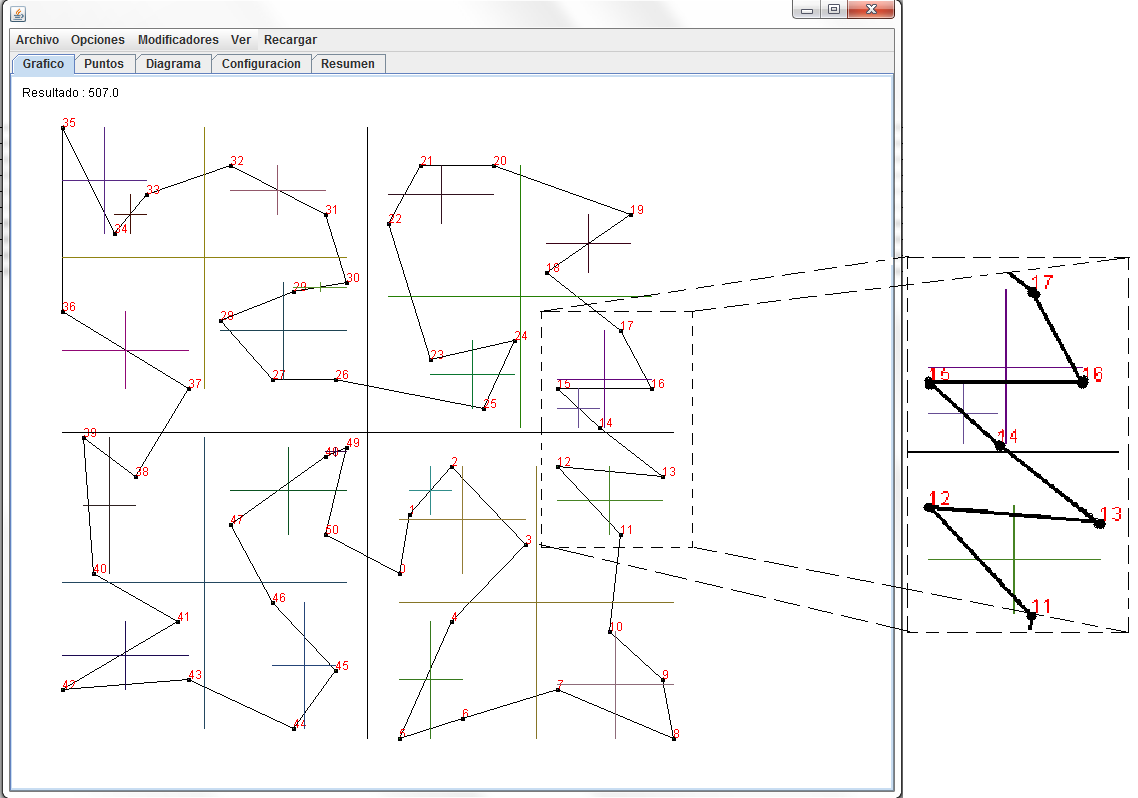
\includegraphics[width=0.7\textwidth]{PruebasResultados/Imagenes/eil51_original_recuadro.png}
            \caption{Problema eil51.tsp resuelto por el método de cuadrantes.}
            \label{fig:eil51_original.png}
    \end{figure}
    
\hspace*{1cm}Como se ha mencionado anteriormente, una especie está formada por 2 arreglos, cada arreglo tiene uno de estos valores: el gen que se encargará de seleccionar uno de los puntos y el cromosoma que indicará hacia donde se desplazará el intercambio; el objetivo de la especie es reordenar los puntos seleccionados, y debido a que ya se resolvió el problema con el método de cuadrantes, no es necesario hacer intercambio con todos los elementos de la lista sino solo con los más cercanos.\\

\hspace*{1cm} En la figura \ref {fig:eil51_explicado.png} se podrá ver que se generó una especie formada por 2 arreglos, una señala al punto 11 y otro al 12,en ambos indica como tipo de cromosoma el número 2. El proceso se dividió en 3 fases:
 \begin{figure}[hbtp]
        \centering
            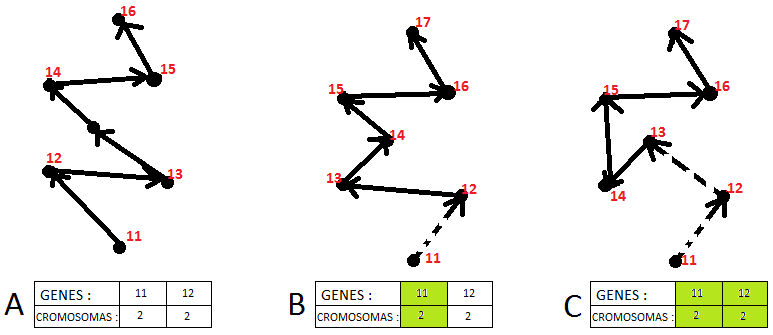
\includegraphics[width=0.75\textwidth]{PruebasResultados/Imagenes/eil51_explicado.png}
            \caption{Problema eil51.tsp resuelto por el método de cuadrantes con una especie aplicada.}
            \label{fig:eil51_explicado.png}
    \end{figure}
\begin{itemize}
    \item \textbf{A:} Éste es el tramo inicial que donde se puede observar que aún no se ha modificado el segmento de la ruta.
    \item \textbf{B:} Aquí se hace el reemplazo, el gen marca el punto 11 y el cromosoma 2, eso quiere decir que el punto 11 tendrá  como siguiente objetivo aquél que este 2 lugares delante de él (13), se intercambiarán las posiciones 12 con el 13, generando una nueva ruta, a diferencia de la fase A, el punto 12 y 13 se encuentran en lugares distintos.
    \item \textbf{C:} Por último se repite lo mostrado en la fase B, esta vez con el nuevo punto 12 y el 14, de nuevo intercambiarán posiciones los puntos 13 y 14 volviendo a generar una nueva ruta.
\end{itemize}

\hspace*{1cm}En la figura \ref {fig:eil51_recocido.png} se muestra la ruta completa con el cambio realizado que tendrá de resultado 502 unidades de distancia, ahorrándose 5 unidades. Este ejemplo es solo hipotético, y para que pueda funcionar se tendrán que hacer varias generaciones de especies, algunos haciendo movimientos para llegar a dicha solución, además de que el reordenamiento puede generar rutas más cortas pero a su vez otras más largas. El objetivo de este procedimiento es ir refinando las especies generadas con el fin de obtener una que mejore la solución obtenida.
     \begin{figure}[hbtp]
        \centering
            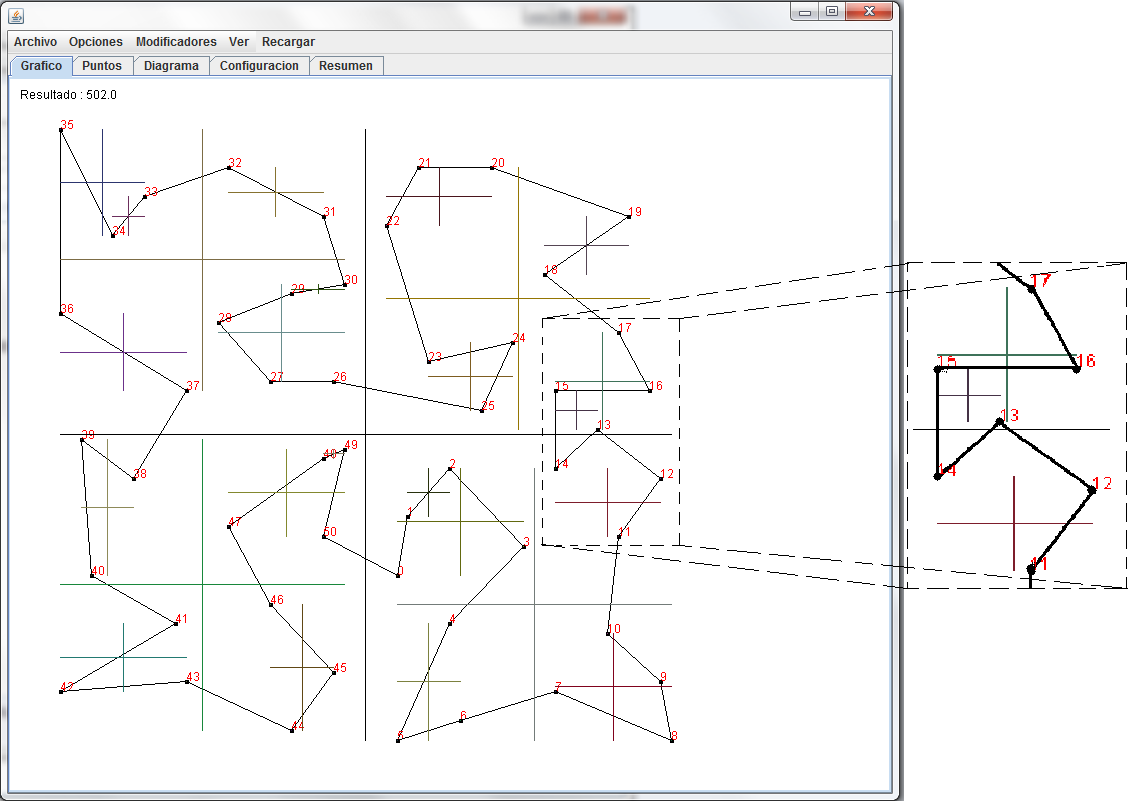
\includegraphics[width=0.7\textwidth]{PruebasResultados/Imagenes/eil51_recocido_recuadro.png}
            \caption{Problema eil51.tsp resuelto por el método de cuadrantes explicando cómo funciona el uso de las especies.}
            \label{fig:eil51_recocido.png}
    \end{figure}    
    \subsection{Metaheurísticas aplicadas en las pruebas}
A continuación se mostrarán las metaheurísticas aplicadas en los experimentos, primero se explicarán los pasos realizados que se muestran en el diagrama de la figura \ref{fig:FLOWCHART2}, después se mostrará la funcionalidad de cada metaheurística programada para este experimento junto con la configuración de parámetros usados en el mismo.
\begin{figure}[hbtp]
   \centering
   \begin{tikzpicture}[node distance=1.6cm]

        \node (start) [startstop] 
		{
				Inicio
		};
        \node (in1) [io, below of=start, text width=5cm] 
		{
        	Recibe un problema de TSP
        };
        \node (pro1) [process, below of=in1, yshift=-0.1cm, text width=12cm] 
		{
        	Resolver el problema por el método de cuadrantes (solución original)
        };       
        \node (pro2) [process, below of=pro1, yshift=-0.1cm, text width=12cm] 
		{
        	Se aplicará una metaheurística (Recocido Simulado, Greedy o Genético) para mutar la solución original
        };    
        \node (in2) [io, below of=pro2, text width=5cm] 
		{
        	Se guardará el resultado obtenido
        };
        \node (pro3) [process, below of=in2, yshift=-0.1cm, text width=12cm] 
		{
        	 Se volverá a mutar la solución original cuantas veces se requiera 
        }; 
        \node (pro4) [process, below of=pro3, yshift=-0.1cm, text width=12cm] 
		{
           De los resultados obtenidos se clasificará el mejor, peor y promedio así mismo se comparará por problema cual fue el mejor de los 3
        }; 
        \node (pro5) [process, below of=pro4, yshift=-0.1cm, text width=12cm] 
		{
           Así mismo se harán experimentos saltándose el método de cuadrantes y se anotarán los resultados en una comparativa diferente
        }; 
        \node (Fin) [startstop, below of=pro5, yshift=-0.1cm,] 
		{
				Fin
		};
        
        \draw [arrow] (start) -- (in1);
        \draw [arrow] (in1) -- (pro1);
        \draw [arrow] (pro1) -- (pro2);
        \draw [arrow] (pro2) -- (in2);
        \draw [arrow] (in2) -- (pro3);
        \draw [arrow] (pro3) -- (pro4);
        \draw [arrow] (pro4) -- (pro5);
        \draw [arrow] (pro5) -- (Fin);
		
    \end{tikzpicture}       
    \caption{Diagrama de flujo del experimento de método de cuadrantes con metaheurísticas.}
    \label{fig:FLOWCHART2}
\end{figure} 
\clearpage \newpage

\subsubsection{Algoritmo de Recocido Simulado}
Aquí se aplicará lo aprendido en el código \ref{lst:recocidosimulado} donde usando un valor de aleatoriedad combinado con la diferencia de resultados obtenidos se irá viendo si el resultado (mejor o peor que el anterior) será el objetivo actual. En la tabla \ref{table:ConfiguracionRS.tsp} se describen las variables usadas y en el código \ref{lst:AlgoritmoRecocidoSimuladoPruebas} se muestra la implementación del algoritmo de Recocido simulado.  

% Please add the following required packages to your document preamble:
% \usepackage[table,xcdraw]{xcolor}
% If you use beamer only pass "xcolor=table" option, i.e. \documentclass[xcolor=table]{beamer}
\begin{table}[hbtp]
\centering
\caption{Configuración de las variables de recocido simulado durante las pruebas.}
\begin{tabular}{llr}
\hline
\rowcolor[HTML]{656565} 
\multicolumn{1}{c}{\cellcolor[HTML]{656565}{\color[HTML]{FFFFFF} \textbf{Nombre}}} & \multicolumn{1}{c}{\cellcolor[HTML]{656565}{\color[HTML]{FFFFFF} \textbf{Descripción}}}                                    & \multicolumn{1}{c}{\cellcolor[HTML]{656565}{\color[HTML]{FFFFFF} \textbf{Valor}}} \\ \hline
Ciclos                                                                             & Cantidad de veces en que se repetirá el proceso                                                                            & 10000                                                                             \\ \hline
Genes máximos                                                                      & \begin{tabular}[c]{@{}l@{}}La cantidad de genes que tendrá la especie durante \\ el proceso de búsqueda local\end{tabular} & 100                                                                               \\ \hline
Distancia gen mínimo                                                               & \begin{tabular}[c]{@{}l@{}}El número mínimo que tendrá en el intercambio de \\ posiciones\end{tabular}                     & 2                                                                                 \\ \hline
Distancia gen máximo                                                               & \begin{tabular}[c]{@{}l@{}}El número máximo que tendrá en el intercambio de \\ posiciones\end{tabular}                     & 5                                                                                 \\ \hline
Temperatura inicial                                                                & Al momento de capturarse se multiplica por $10^{-10}$                                        								& 600                                                                               \\ \hline
\end{tabular}

\label{table:ConfiguracionRS.tsp}
\end{table} 

\begin{lstlisting}[language=C++, caption=Algoritmo de recocido simulado aplicado en las pruebas, label=lst:AlgoritmoRecocidoSimuladoPruebas]
    Inicio
    
    Ciclos
    Genes máximos
    Distancia gen mínimo
    Distancia gen máximo
    Factor de temperatura
    
    Recibir una lista de puntos para trabajar convirtiéndose en la lista de puntos actual.
    MIENTRAS(NO se hayan cumplido la cantidad de Ciclos){
    	1.- Crear una nueva especie con una longitud igual a la cantidad de genes máximos.
    	2.- Los números que conformara la especie oscilara entre el número mínimo y máximo declarados anteriormente.
    	3.- Una vez declarada alterara la lista de puntos actual para obtener una lista nueva.
    	4.- Una vez alterada la lista de puntos actual con la nueva, en caso de obtener un mejor resultado 
    	SI(el resultado es mejor){
    		1.-esta lista es sustituida por la nueva.
    	}SINO{
    		1.-Aplicar formula de temperatura
    		SI(APLICA){
    		    1.-La especie, aunque ineficiente se convierte en la lista de puntos actual.
    		    2.-Se ajusta la temperatura.
    		}
    	}
    }
    
    Fin
\end{lstlisting}

\clearpage \newpage

\subsubsection{Algoritmo Greedy}
A diferencia del algoritmo de recocido simulado, el algoritmo Greedy (o voraz) es más directo, intenta sacar al azar una solución y verifica que éste sea el mejor, si lo es sustituye al original, sino lo es lo descarta y continua el proceso hasta que se cumpla el criterio de paro, que en este caso son el número de veces (o ciclos) que se repetirá el proceso. En la tabla \ref{table:ConfiguracionGR.tsp} se describen las variables usadas y en el código \ref{lst:AlgoritmoGreedyPruebas} muestra la implementación del algoritmo Greedy.

% Please add the following required packages to your document preamble:
% \usepackage[table,xcdraw]{xcolor}
% If you use beamer only pass "xcolor=table" option, i.e. \documentclass[xcolor=table]{beamer}
\begin{table}[hbtp]
\centering
\caption{Configuración de las variables de método greedy durante las pruebas.}
\begin{tabular}{llr}
\hline
\rowcolor[HTML]{656565} 
\multicolumn{1}{c}{\cellcolor[HTML]{656565}{\color[HTML]{FFFFFF} \textbf{Nombre}}} & \multicolumn{1}{c}{\cellcolor[HTML]{656565}{\color[HTML]{FFFFFF} \textbf{Descripción}}}                                    & \multicolumn{1}{c}{\cellcolor[HTML]{656565}{\color[HTML]{FFFFFF} \textbf{Valor}}} \\ \hline
Ciclos                                                                             & Cantidad de veces en que se repetirá el proceso.                                                                            & 10000                                                                             \\ \hline
Genes máximos                                                                      & \begin{tabular}[c]{@{}l@{}}La cantidad de genes que tendrá la especie durante \\ el proceso de búsqueda local.\end{tabular} & 100                                                                               \\ \hline
Distancia gen mínimo                                                               & \begin{tabular}[c]{@{}l@{}}El número mínimo que tendrá el intercambio de \\ posiciones.\end{tabular}                     & 2                                                                                 \\ \hline
Distancia gen máximo                                                               & \begin{tabular}[c]{@{}l@{}}El número máximo que tendrá el intercambio de \\ posiciones.\end{tabular}                     & 5                                                                                 \\ \hline
\end{tabular}
\label{table:ConfiguracionGR.tsp}
\end{table} 

\begin{lstlisting}[language=C++, caption=Algoritmo greedy aplicado en las pruebas, label=lst:AlgoritmoGreedyPruebas]
    Inicio
    
    Ciclos
    Genes máximos
    Distancia gen mínimo
    Distancia gen máximo
    
    Recibir una lista de puntos para trabajar convirtiéndose en la lista de puntos actual.
    MIENTRAS(NO se hayan cumplido la cantidad de Ciclos){
    	1.- Crear una nueva especie con una longitud igual a la cantidad de genes máximos
    	2.- Los números que conformará la especie oscilará entre el número mínimo y máximo declarados anteriormente
    	3.- Una vez declarada alterara la lista de puntos actual para obtener una lista nueva.
    	4.- Una vez alterada la lista de puntos actual con la nueva, en caso de obtener un mejor resultado esta lista es sustituida por la nueva
    }
    
    Fin
\end{lstlisting}

\clearpage \newpage

\subsubsection{Algoritmo Genético}
Por último el algoritmo genético en vez de modificar una solución candidata, utiliza una población de ellas donde soluciones con mejor resultado tendrá la prioridad para reproducirse, y durante varias generaciones los descendientes irán modificando el resultado original hasta que al final devuelva uno mejor. Entre los aspectos a destacar son el hecho de dividir los genes en dominantes y recesivos: los primeros jamás se modificarán y representan aquellos cambios que son capaces de mejorar el resultado y luego están los recesivos que estarán sujetos a una mutación devolviendo otro conjuntos de valores numéricos que pueden o no mejorar la solución. En la tabla \ref{table:ConfiguracionAG.tsp} se describen las variables usadas y en el código \ref{lst:AlgoritmoGeneticoPruebas} muestra la implementación del algoritmo genético.

% Please add the following required packages to your document preamble:
% \usepackage[table,xcdraw]{xcolor}
% If you use beamer only pass "xcolor=table" option, i.e. \documentclass[xcolor=table]{beamer}
\begin{table}[hbtp]
\centering
\caption{Configuración de las variables de algoritmo genético durante las pruebas.}
\begin{tabular}{
>{\columncolor[HTML]{FFFFFF}}l lr}
\hline
\multicolumn{1}{c}{\cellcolor[HTML]{656565}{\color[HTML]{FFFFFF} \textbf{Nombre}}} & \multicolumn{1}{c}{\cellcolor[HTML]{656565}{\color[HTML]{FFFFFF} \textbf{Descripción}}}                                                                                                          & \cellcolor[HTML]{656565}{\color[HTML]{FFFFFF} \textbf{Valor}} \\ \hline
Generaciones                                                                       & \begin{tabular}[c]{@{}l@{}}Cantidad de veces que se repetirá el proceso, en \\ este caso la cantidad de nuevas generaciones de hijos.\end{tabular}                                                & 1000                                                          \\ \hline
{\color[HTML]{000000} Población}                                                   & \begin{tabular}[c]{@{}l@{}}Cantidad máxima que tendrá cada generación, en caso \\ de ser impar se eliminará el único que quede sin pareja \\ durante el proceso de cruza.\end{tabular}            & 100                                                           \\ \hline
{\color[HTML]{000000} Genes máximos}                                               & \begin{tabular}[c]{@{}l@{}}La cantidad de genes que tendrá la especie durante \\ el proceso de búsqueda local.\end{tabular}                                                                       & 100                                                           \\ \hline
{\color[HTML]{000000} Distancia gen mínimo}                                        & \begin{tabular}[c]{@{}l@{}}El número mínimo que tendrá el intercambio de \\ posiciones.\end{tabular}                                                                                           & 2                                                             \\ \hline
{\color[HTML]{000000} Distancia gen máximo}                                        & \begin{tabular}[c]{@{}l@{}}El número máximo que tendrá el intercambio de \\ posiciones.\end{tabular}                                                                                           & 5                                                             \\ \hline
\begin{tabular}[c]{@{}l@{}}Rango de mutación \\ mínimo\end{tabular}                & \begin{tabular}[c]{@{}l@{}}Porcentaje aleatorio mínimo de genes recesivos \\ que serán modificados durante la mutación,\\ esta cantidad se calcula junto con el valor de \\ genes máximos.\end{tabular} & 10                                                            \\ \hline
\begin{tabular}[c]{@{}l@{}}Rango de mutación \\ máximo\end{tabular}                & \begin{tabular}[c]{@{}l@{}}Porcentaje aleatorio máximo de genes recesivos \\ que serán modificados durante la mutación,\\ esta cantidad se calcula junto con el valor de \\ genes mínimos.\end{tabular} & 40                                                            \\ \hline
\end{tabular}
\label{table:ConfiguracionAG.tsp}
\end{table}

\begin{lstlisting}[language=C++, caption=Algoritmo genético aplicado en las pruebas, label=lst:AlgoritmoGeneticoPruebas]
    Inicio
        
    Generaciones
    Población
    Genes máximos
    Distancia gen mínimo
    Distancia gen máximo
    Rango de mutación mínimo
    Rango de mutación máximo
    
    1.-Recibir una lista de puntos para trabajar convirtiéndose en la lista de puntos actual.
    
    MIENTRAS(NO se hayan creado la cantidad de Generaciones establecidas)
    {
    
    	1.-Se crea una nueva población conformada de Especies.
    	
    	2.-Cada Especie tiene una cantidad de genes igual al valor de genes máximos y sus valores oscilan entre los números máximos y mínimos de distancia.
    	
    	3.-Todas las especies se cruzan con la lista de puntos actual, se ordenan de acuerdo a su desempeño.
    	
    	4.-Si mejor especie supera a la solución actual, es reemplazada, de lo contrario la solución actual permanecerá dentro de la población sustituyendo a la solución más débil.
    	
    	5.-Una vez que se haya terminado la evaluación se procederá el siguiente paso.
    	
    	MIENTRAS (Existan Especies sin pareja)
    	{
    	
    		1.- La mejor especie selecciona al azar cualquier miembro de la población convirtiéndose en padre y madre de la siguiente especie.
    		
    		2.- Este hijo sera el resultado de la combinación de los genes en posiciones pares del padre y los genes de las posiciones impares de la madre.
    		
    		3.- Los genes que ayuden a mejorar el rendimiento de la solución se llamaran dominantes mientras que los que afecten se llamaran recesivos.
    		
    		4.- Los genes recesivos se someterán a un proceso de mutación, donde sus valores serán alterados de acuerdo a las distancias mínimas y máximas, la cantidad de genes mutados será determinado por los rangos mínimos y máximos de mutación.
    		
    		5.- El hijo sera agregado a la nueva población y los padres serán descartados.
    		
    		6.- El proceso se repite esta vez con la siguiente mejor Especie.
    		
    	}
    	
    }
               
    Fin
\end{lstlisting}

\clearpage \newpage

\subsection{Experimentos}
A continuación se presenta una breve explicación de los elementos que compondrán los experimentos. Se llevaron a cabo 15 experimentos con las instancias de la TSPLIB. Se hicieron 100 corridas de cada problema con el fin de obtener diferentes resultados. Todos los experimentos mantienen la misma configuración y se prefirió no ajustarla con el fin de asegurar el mismo rendimiento en ambos problemas.\\
Los datos arrojados quedaron registrados en las siguientes 3 presentaciones:\\

\begin{enumerate}[label=\Alph*.-]
\item Una tabla comparativa del mismo experimento (figura \ref {fig:ExplicacionExperimento_A.png}) que muestra los resultados agrupados por tipo de metaheurística y si se aplicó o no el método de cuadrantes. Las celdas coloreadas ayuda a representar entre los 3 el mejor resultado, el mejor porcentaje y de los peores resultados el más pequeño.
\item Una imagen comparativa del resultado original (sin aplicar metaheurísticas) y otro que muestra el mejor resultado usando la metaheurística ganadora (en ambos están aplicando el método de cuadrantes). Como se puede observar en la figura \ref {fig:ExplicacionExperimento_B.png}, los círculos marcados muestran los puntos cuyo orden es distinto en comparación a la imagen de la izquierda.
\item Una gráfica comparativa mostrando los resultados de las 100 corridas (figura \ref {fig:ExplicacionExperimento_C.png}) que están ordenados de manera descendente para observar el progreso comparado con las demás metaheurísticas. Esta gráfica muestra los resultados obtenidos aplicando o no el método de cuadrantes.
\end{enumerate}

\clearpage \newpage

\begin{figure}[hbtp]
    \centering
        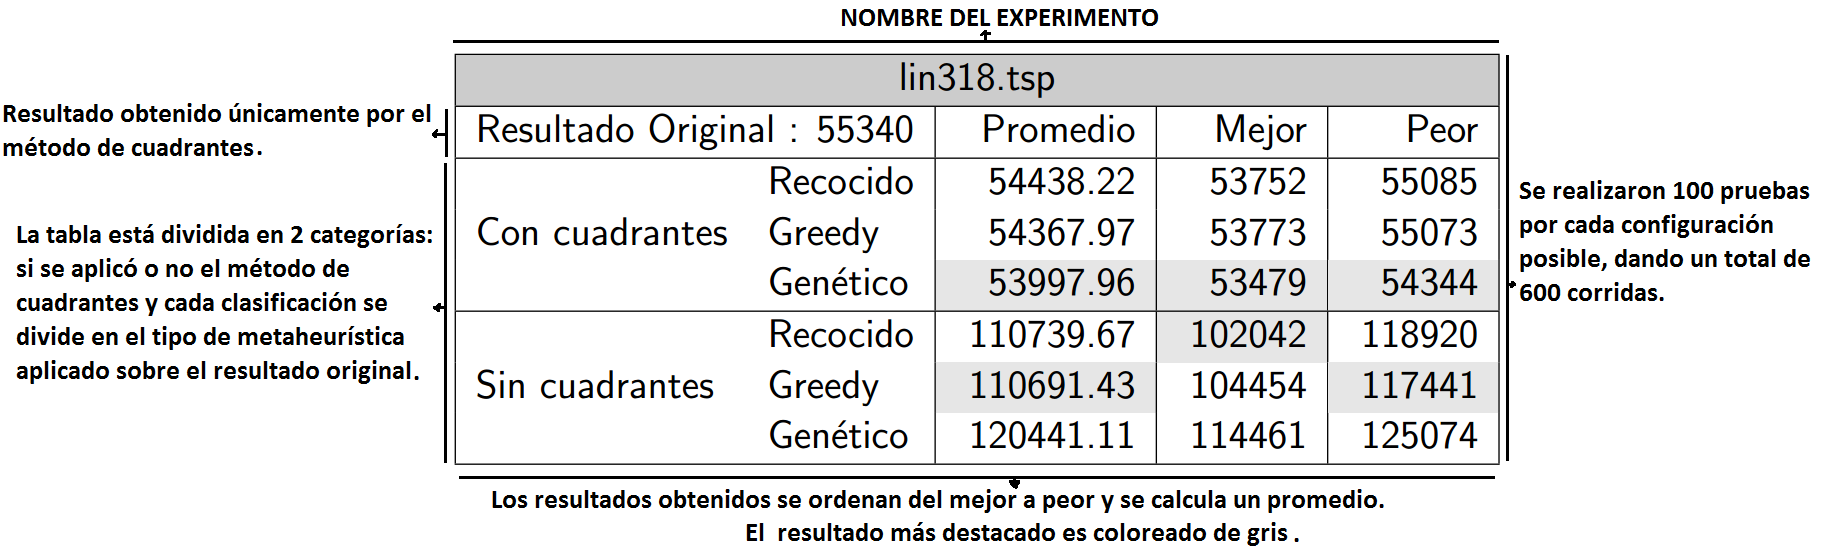
\includegraphics[width=1\textwidth]{PruebasResultados/Imagenes/ExplicacionExperimento_A.png}
        \caption{Explicación del experimento (punto A), tabla comparativa.}
        \label{fig:ExplicacionExperimento_A.png}
\end{figure}

\begin{figure}[hbtp]
    \centering
        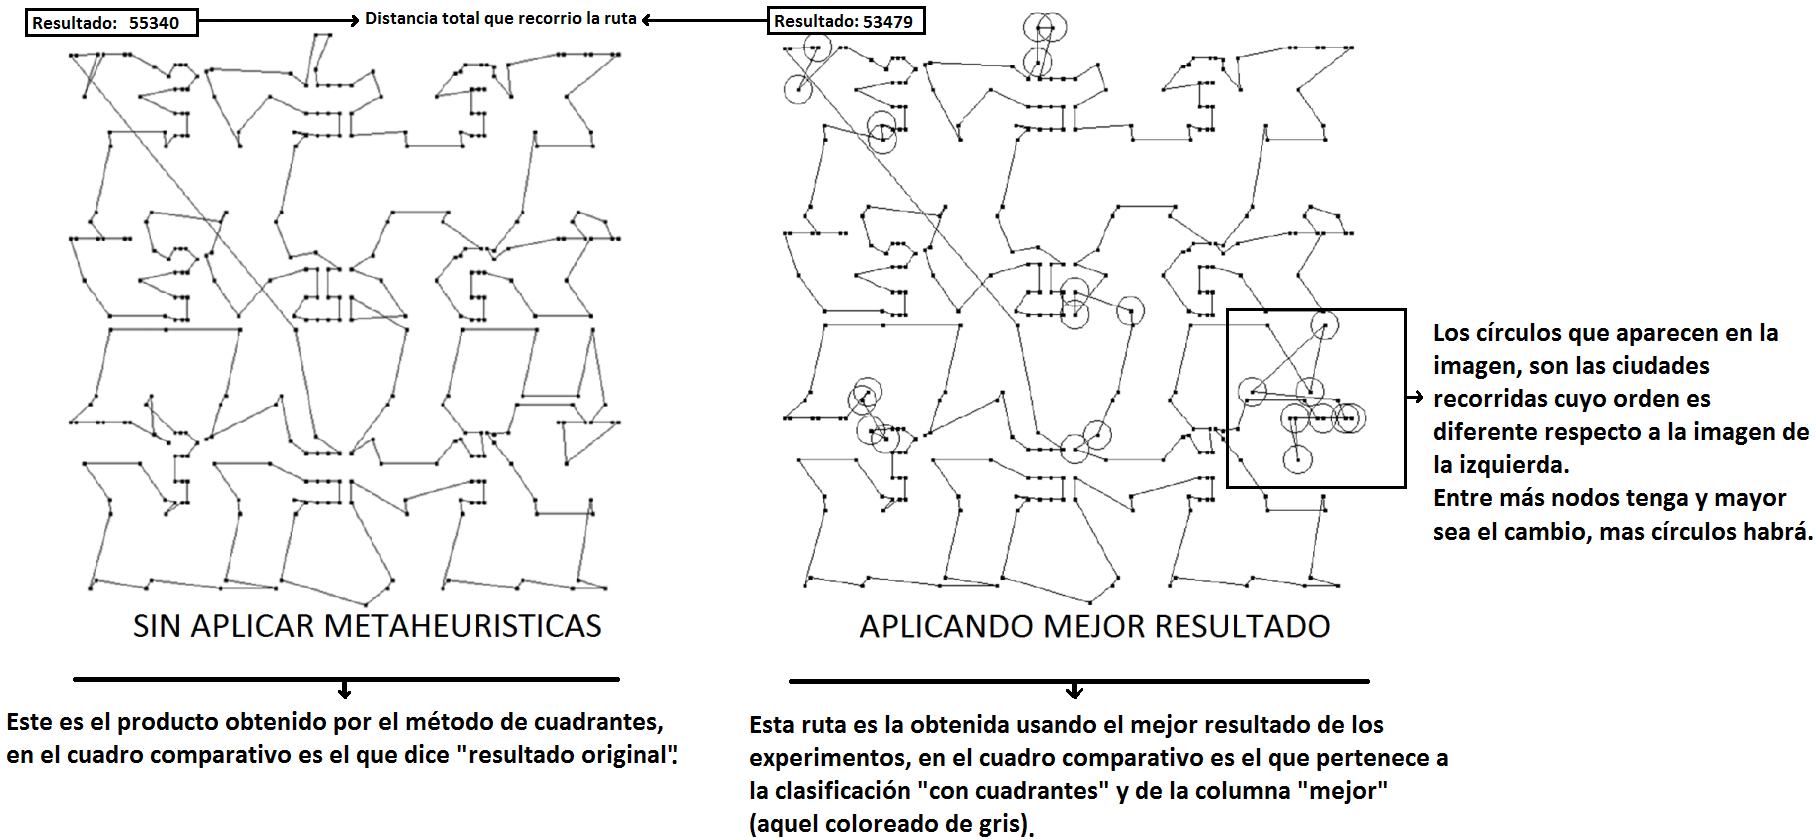
\includegraphics[width=1\textwidth]{PruebasResultados/Imagenes/ExplicacionExperimento_B.png}
        \caption{Explicación del experimento (punto B), comparación de rutas.}
        \label{fig:ExplicacionExperimento_B.png}
\end{figure}

\begin{figure}[hbtp]
    \centering
        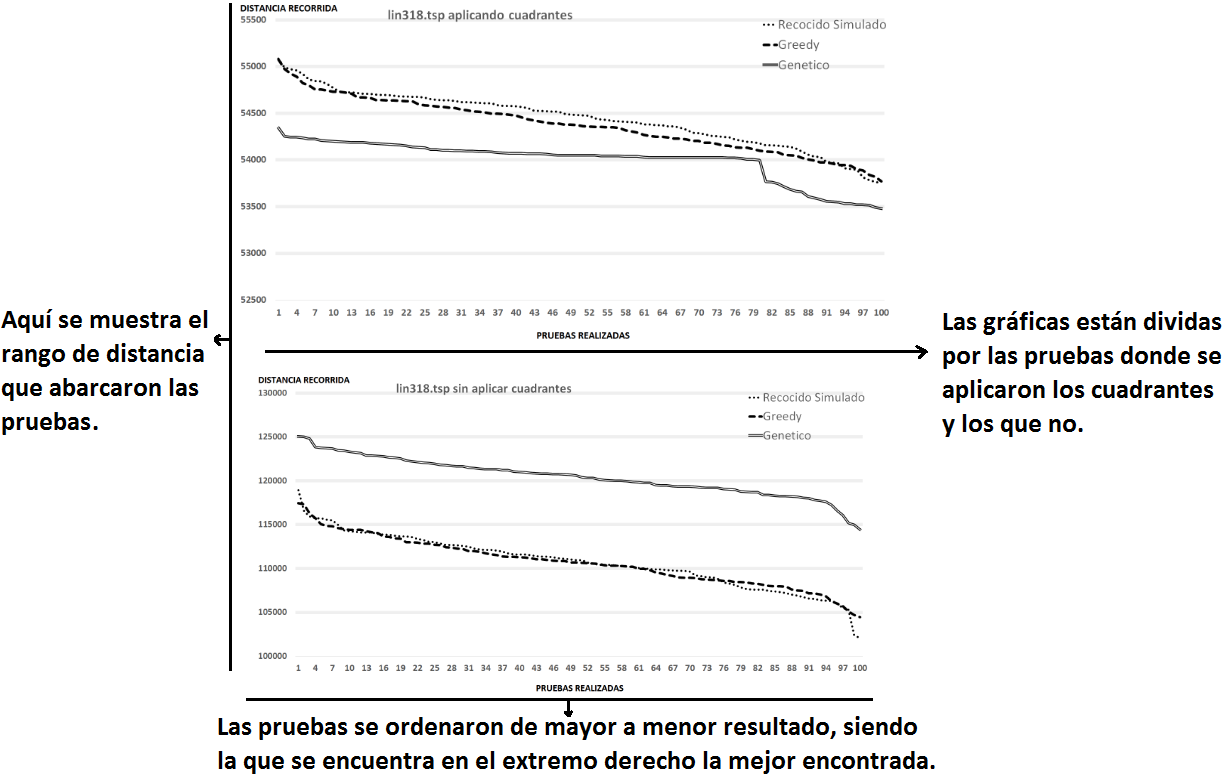
\includegraphics[width=1\textwidth]{PruebasResultados/Imagenes/ExplicacionExperimento_C.png}
        \caption{Explicación del experimento (punto C), gráfica que compara los resultados obtenidos aplicando o no el método de cuadrantes.}
        \label{fig:ExplicacionExperimento_C.png}
\end{figure}

\clearpage \newpage
    
%A280.TSP
\subsubsection{a280.TSP}
\begin{table}[hbtp]
    \centering
    \caption{Experimento con el problema a280.TSP.}    
    \small
    \begin{tabular}{| l   l | r | r | r |   }
    \hline\multicolumn{5}{|c|}{ \rowcolor[gray]{0.8}a280.TSP} \\\hline
    \multicolumn{2}{|l|}{Resultado Original : 3418}   & Promedio & Mejor & Peor \\ 
                \hline
                & Recocido  &  3364.17 & 3329 & \cellcolor[gray]{0.9} 3394  \\ 
Con cuadrantes  & Greedy    &  3363.79 & 3335 & 3396  \\ 
                & Genético  & \cellcolor[gray]{0.9} 3354.06 & \cellcolor[gray]{0.9} 3318 & 3418 \\ 
                    \hline
                & Recocido  &  5078.51 & \cellcolor[gray]{0.9} 4711 & 5345   \\ 
Sin cuadrantes  & Greedy    &  5101.88 & 4804 & 5410   \\ 
                & Genético  &  \cellcolor[gray]{0.9} 4876.34 & 4747 & \cellcolor[gray]{0.9} 5066 \\ 
                    \hline
    \end{tabular}
    \label{table:EXP_a280.TSP}
\end{table}
 \begin{figure}[hbtp]
    \centering
        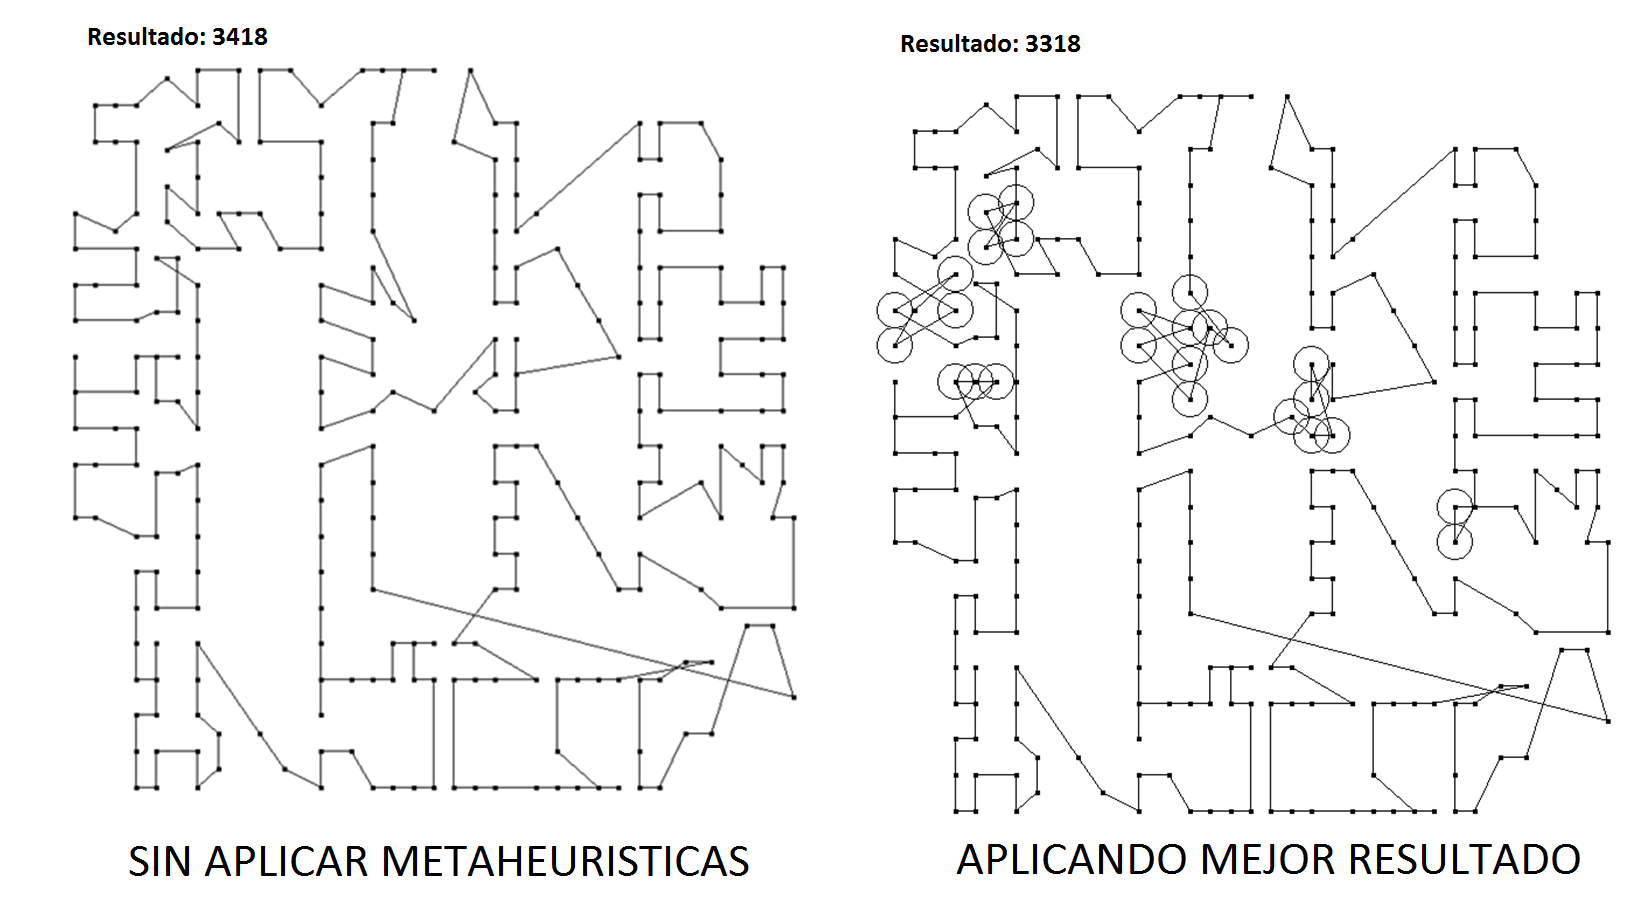
\includegraphics[width=1\textwidth]{PruebasResultados/Experimentos_Comparativas/a280.png}
        \caption{Comparativa a280.tsp.}
        \label{fig:a280_comparativa.png}
\end{figure}
 \begin{figure}[hbtp]
    \centering
        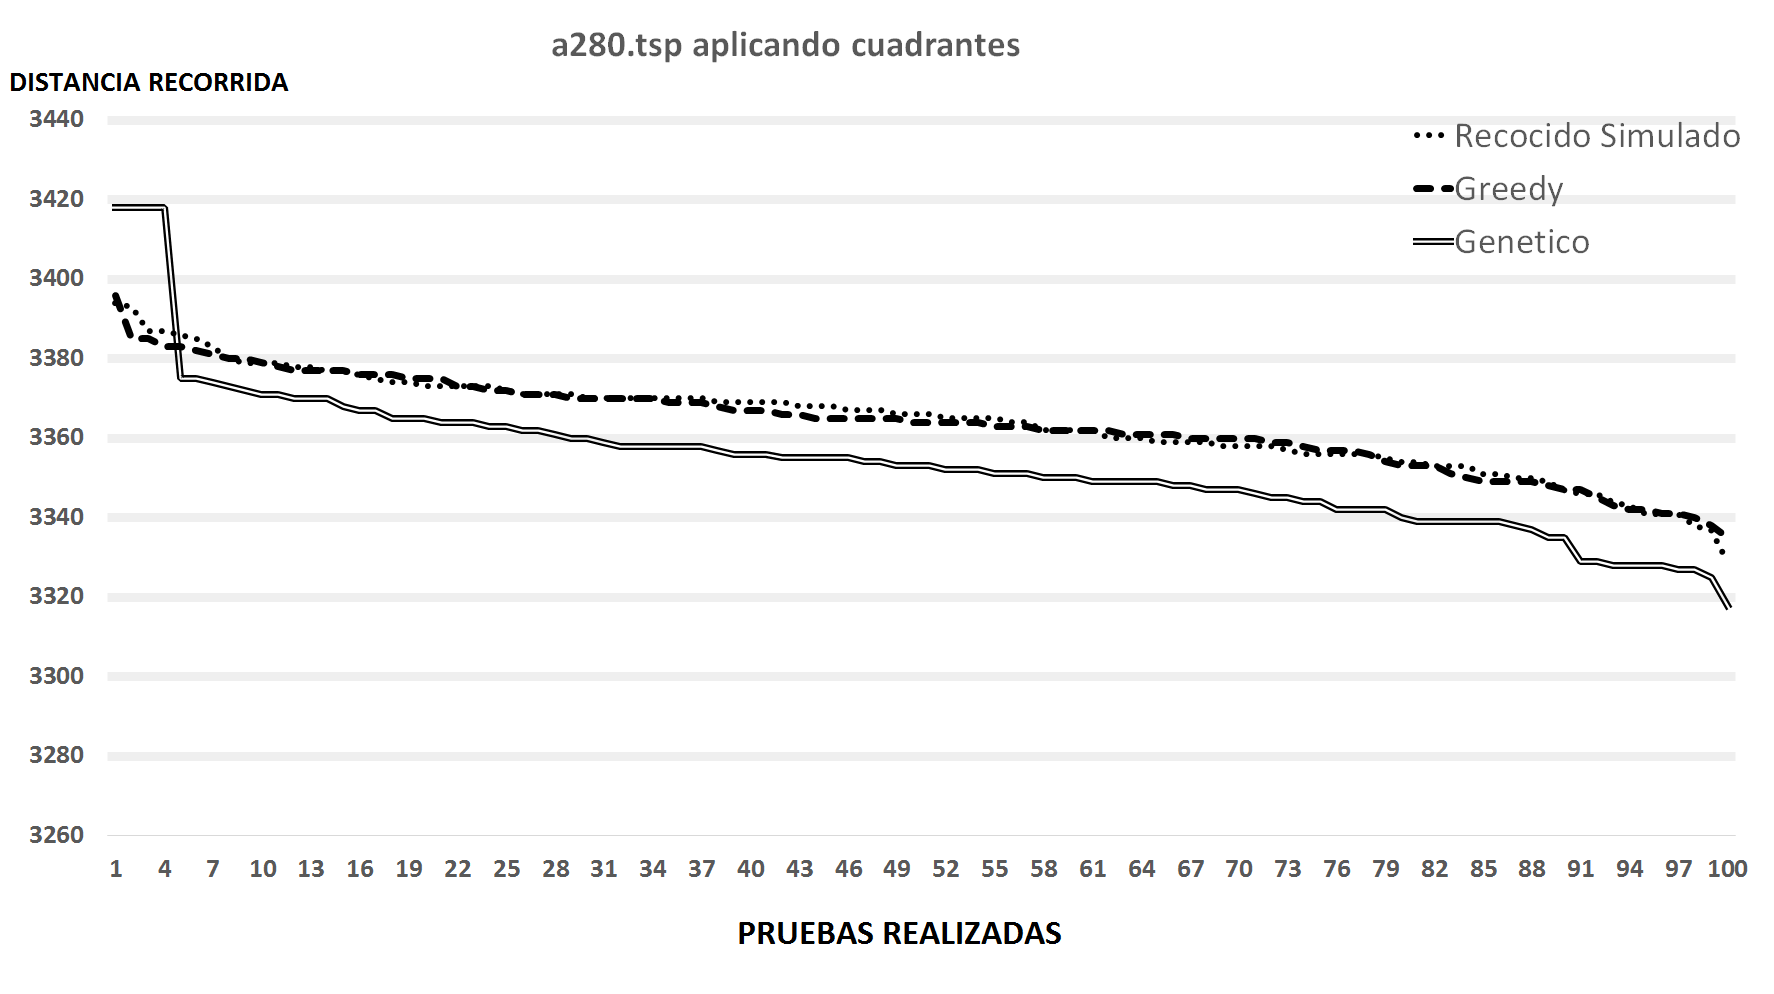
\includegraphics[width=1\textwidth]{PruebasResultados/Experimentos_Graficos_Con/a280.png}
        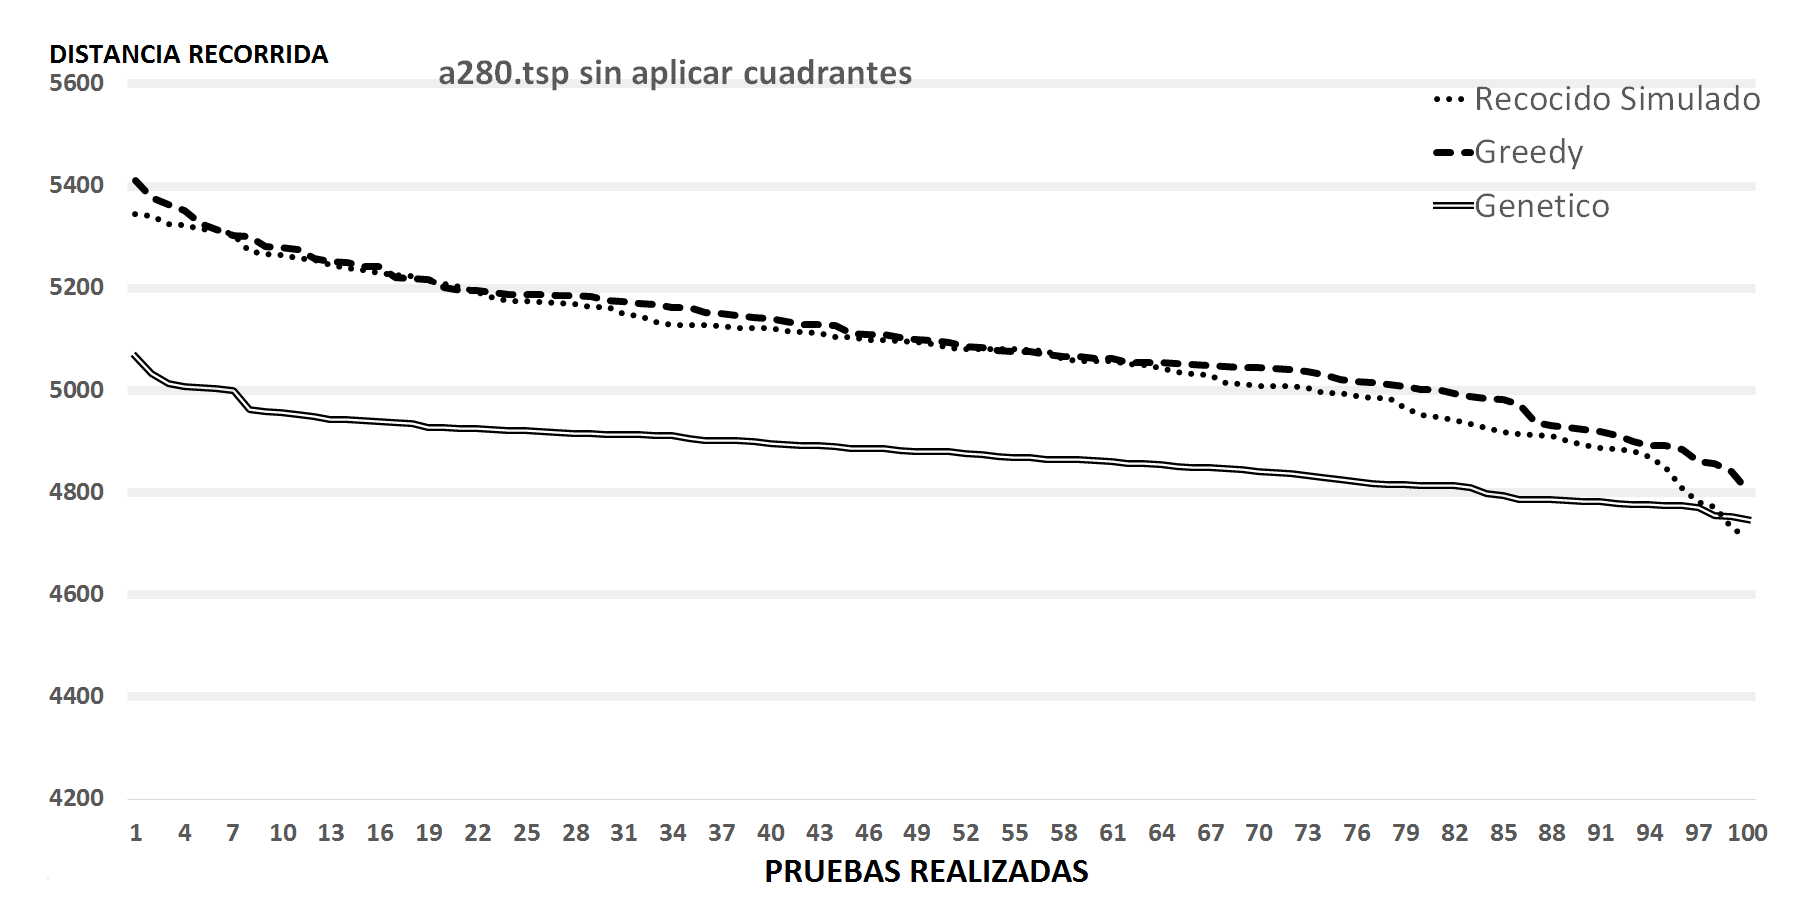
\includegraphics[width=1\textwidth]{PruebasResultados/Experimentos_Graficos_Sin/a280.png}
        \caption{Gráficos a280.tsp con cuadrantes y sin cuadrantes.}
        \label{fig:a280_grafica.png}
\end{figure}
\newpage

\hspace*{1cm}Como se puede observar en la figura \ref{fig:a280_explicado.png}, los círculos marcan las zonas mutadas de la solución obtenida mediante el método de cuadrantes. En la figura \ref{fig:a280_comparativa.png} algunos puntos que se muestran en la imagen de la derecha están encerrados en círculos, estos puntos están marcados así porque fueron colocados fuera de la posición original que se le asignó por el método de cuadrantes.\\
\hspace*{1cm}Regresando a la figura \ref{fig:a280_explicado.png} se puede ver 3 imágenes:
\begin{itemize}
    \item \textbf{A: }Es el problema resuelto por el método de cuadrantes.
    \item \textbf{B: }El mismo problema, solo que fue modificado usando metaheurísticas, aquí se puede apreciar que varios puntos fueron encerrados en círculos ya comentando su funcionalidad 
    \item \textbf{C: }Es la imagen B sin los puntos marcados, para que se puede apreciar con mejor detalle las diferencias que tiene con la imagen A.
\end{itemize}

\begin{figure}[hbtp]
    \centering
        \includegraphics[width=1\textwidth]{PruebasResultados/Imagenes/a280_explicado.png}
        \caption{Explicación de los cambios realizados en el a280.tsp.}
        \label{fig:a280_explicado.png}
\end{figure}

\hspace*{1cm}Ya conociendo para que sirve esta imagen se procederá con los demás experimentos.

\newpage

%brd14051.TSP
\subsubsection{brd14051.TSP}
\begin{table}[hbtp]
    \centering 
    \caption{Experimento con el problema brd14051.tsp.}    
	\begin{tabular}{ | l   l | r | r | r |   }
    \hline\multicolumn{5}{|c|}{ \rowcolor[gray]{0.8}brd14051.tsp} \\\hline
    \multicolumn{2}{|l|}{Resultado Original :623324}  & Promedio & Mejor & Peor \\ 
                \hline
                & Recocido  & \cellcolor[gray]{0.9} 619876.89 & \cellcolor[gray]{0.9} 618878 & \cellcolor[gray]{0.9} 620546 \\ 
 Con cuadrantes & Greedy    & 619899.03 & 619060 & 620743  \\ 
                & Genético  & 621842.30 & 621273 & 622688  \\ 
                \hline
                & Recocido  & 13091307.46 & \cellcolor[gray]{0.9} 12612710 & 13458979 \\ 
 Sin cuadrantes & Greedy    & \cellcolor[gray]{0.9} 13071094.56 & 12811921 & \cellcolor[gray]{0.9} 13411800 \\ 
                & Genético  & 23478563.40 & 23433764 & 23520252 \\ 
                \hline
    \end{tabular}
    \label{table:EXP_brd14051.tsp}
\end{table}
\begin{figure}[hbtp]
    \centering
        \includegraphics[width=1\textwidth]{PruebasResultados/Experimentos_Comparativas/brd14051.png}
        \caption{Comparativa brd14051.tsp.}
        \label{fig:brd14051_comparativa.png}
\end{figure}
 \begin{figure}[hbtp]
    \centering
        \includegraphics[width=1\textwidth]{PruebasResultados/Experimentos_Graficos_Con/brd14051.png}
        \includegraphics[width=1\textwidth]{PruebasResultados/Experimentos_Graficos_Sin/brd14051.png}
        \caption{Gráficos brd14051.tsp con cuadrantes y sin cuadrantes.}         
        \label{fig:brd14051_grafica.png} 
\end{figure}
\newpage

%CH150.TSP
\subsubsection{ch150.TSP}
\begin{table}[hbtp]
 \centering	
    \caption{Experimento con el problema ch150.tsp.} 
	\begin{tabular}{ | l   l | r | r | r |   }
         \hline\multicolumn{5}{|c|}{ \rowcolor[gray]{0.8} ch150.tsp } \\\hline
         \multicolumn{2}{|l|}{Resultado Original : 8579}   & Promedio & Mejor & Peor \\ 
                \hline
                & Recocido  &  8445.98 & 8272 & 8535  \\ 
 Con cuadrantes & Greedy    &  8446.02 & 8315 & 8540  \\ 
                & Genético  & \cellcolor[gray]{0.9}8358.81 & \cellcolor[gray]{0.9}8231 & \cellcolor[gray]{0.9}8427 \\ 
                \hline
                & Recocido  & \cellcolor[gray]{0.9} 26500.85 & 23162 & \cellcolor[gray]{0.9} 28674 \\ 
 Sin cuadrantes & Greedy    &  26614.55 & \cellcolor[gray]{0.9} 22417 & 29187 \\ 
                & Genético  &  34548.11 & 32091 & 37844 \\ 
                \hline
    \end{tabular}
    \label{table:EXP_ch150.tsp}
\end{table}
\begin{figure}[hbtp]
    \centering
        \includegraphics[width=1\textwidth]{PruebasResultados/Experimentos_Comparativas/ch150.png}
        \caption{Comparativa ch150.tsp.}
        \label{fig:ch150_comparativa.png}
\end{figure}
 \begin{figure}[hbtp]
    \centering
        \includegraphics[width=1\textwidth]{PruebasResultados/Experimentos_Graficos_Con/ch150.png}
        \includegraphics[width=1\textwidth]{PruebasResultados/Experimentos_Graficos_Sin/ch150.png}
        \caption{Gráficos ch150.tsp con cuadrantes y sin cuadrantes.}
        \label{fig:ch150_grafica.png}
\end{figure}
\newpage

%d1655.TSP
\subsubsection{d1655.TSP}
\begin{table}[hbtp]
 \centering 
    \caption{Experimento con el problema d1655.tsp.} 
	\begin{tabular}{ | l   l | r | r | r |   }
         \hline\multicolumn{5}{|c|}{ \rowcolor[gray]{0.8}d1655.tsp} \\ \hline
         \multicolumn{2}{|l|}{Resultado Original :83605}  & Promedio & Mejor & Peor \\ 
                \hline
                & Recocido  & 82500.78 & 82098 & 82881 \\ 
 Con cuadrantes & Greedy    & 82489.63 & 82014 & 82839 \\ 
                & Genético  & \cellcolor[gray]{0.9} 82244 & \cellcolor[gray]{0.9} 81996 & \cellcolor[gray]{0.9} 82447 \\ 
                \hline
                & Recocido  & 235605.87 & \cellcolor[gray]{0.9} 222473 & \cellcolor[gray]{0.9} 243750 \\ 
 Sin cuadrantes & Greedy    & 236306.2 & 226740 & 246172 \\ 
                & Genético  & \cellcolor[gray]{0.9} 264556.11 & 262348 & 266415 \\ 
                \hline
    \end{tabular}
    \label{table:EXP_d1655.tsp}
\end{table}
\begin{figure}[hbtp]
    \centering
        \includegraphics[width=1\textwidth]{PruebasResultados/Experimentos_Comparativas/d1655.png}
        \caption{Comparativa d1655.tsp.}
        \label{fig:d1655_comparativa.png}
\end{figure}
 \begin{figure}[hbtp]
    \centering
        \includegraphics[width=1\textwidth]{PruebasResultados/Experimentos_Graficos_Con/d1655.png}
        \includegraphics[width=1\textwidth]{PruebasResultados/Experimentos_Graficos_Sin/d1655.png}
        \caption{Gráficos d1655.tsp con cuadrantes y sin cuadrantes.}
        \label{fig:d1655_grafica.png}
\end{figure}
\newpage

%D493.TSP
\subsubsection{d493.TSP}
\begin{table}[hbtp]
 \centering 
    \caption{Experimento con el problema d493.tsp.}
	\begin{tabular}{ | l   l | r | r | r |   }
        \hline\multicolumn{5}{|c|}{ \rowcolor[gray]{0.8} d493.tsp} \\ \hline
        \multicolumn{2}{|l|}{Resultado Original : 45731} & Promedio & Mejor & Peor \\ 
                \hline
                & Recocido  & 44582.69 & 44124 & 45012  \\ 
 Con cuadrantes & Greedy    & 44604.21 & 44054 & 45275  \\ 
                & Genético  & \cellcolor[gray]{0.9} 43987.43 & \cellcolor[gray]{0.9} 43373 & \cellcolor[gray]{0.9} 44918  \\ 
                \hline
                & Recocido  & 96827.13 & 91468 & 102751   \\ 
 Sin cuadrantes & Greedy    & \cellcolor[gray]{0.9} 96002.89 & \cellcolor[gray]{0.9} 89956 & \cellcolor[gray]{0.9} 100955   \\ 
                & Genético  & 121326.2 & 115991 & 124989    \\ 
                \hline
    \end{tabular}
    \label{table:EXP_d493.tsp}
\end{table}
\begin{figure}[hbtp]
    \centering
        \includegraphics[width=1\textwidth]{PruebasResultados/Experimentos_Comparativas/d493.png}
        \caption{Comparativa d493.tsp.}
        \label{fig:d493_comparativa.png}
\end{figure}
 \begin{figure}[hbtp]
    \centering
        \includegraphics[width=1\textwidth]{PruebasResultados/Experimentos_Graficos_Con/d493.png}
        \includegraphics[width=1\textwidth]{PruebasResultados/Experimentos_Graficos_Sin/d493.png}
        \caption{Gráficos d493.tsp con cuadrantes y sin cuadrantes.}
        \label{fig:d493_grafica.png}
\end{figure}
\newpage

%EIL101.TSP
\subsubsection{eil101.TSP}
\begin{table}[hbtp]
 \centering
     \caption{Experimento con el problema eil101.tsp.}
\begin{tabular}{ | l   l | r | r | r |   }
	    \hline\multicolumn{5}{|c|}{ \rowcolor[gray]{0.8} eil101.tsp} \\ \hline
         \multicolumn{2}{|l|}{Resultado Original : 828}   & Promedio & Mejor & Peor \\ 
                \hline
                & Recocido  & 804.91 & 788 & 822  \\ 
 Con cuadrantes & Greedy    & 806.93 & 788 & 825  \\ 
                & Genético  & \cellcolor[gray]{0.9} 787.33 & \cellcolor[gray]{0.9} 781 & \cellcolor[gray]{0.9} 802  \\ 
                \hline
                & Recocido  & 1747.41 & \cellcolor[gray]{0.9} 1585 & 1917   \\ 
 Sin cuadrantes & Greedy    & 1744.97 & 1630 & 1855   \\ 
                & Genético  & \cellcolor[gray]{0.9} 1705.49 & 1602 & \cellcolor[gray]{0.9} 1740    \\ 
                \hline
    \end{tabular}
    \label{table:EXP_eil101.tsp}
\end{table}
 \begin{figure}[hbtp]
    \centering
        \includegraphics[width=1\textwidth]{PruebasResultados/Experimentos_Comparativas/eil101.png}
        \caption{Comparativa eil101.tsp.}
        \label{fig:eil101_comparativa.png}
\end{figure}
 \begin{figure}[hbtp]
    \centering
        \includegraphics[width=1\textwidth]{PruebasResultados/Experimentos_Graficos_Con/eil101.png}
        \includegraphics[width=1\textwidth]{PruebasResultados/Experimentos_Graficos_Sin/eil101.png}
        \caption{Gráficos eil101.tsp con cuadrantes y sin cuadrantes.}
        \label{fig:eil101_grafica.png}
\end{figure}
\newpage

%fl417.TSP
\subsubsection{fl417.TSP}
\begin{table}[hbtp]
 \centering 
    \caption{Experimento con el problema fl417.tsp.}
	\begin{tabular}{ | l   l | r | r | r |   }
       \hline\multicolumn{5}{|c|}{ \rowcolor[gray]{0.8} fl417.tsp} \\\hline
        \multicolumn{2}{|l|}{Resultado Original : 17419} & Promedio & Mejor & Peor \\ 
                \hline
                & Recocido  & 16835.95 & 16672 & 17070  \\ 
 Con cuadrantes & Greedy    & 16824.81 & 16610 & 17028  \\ 
                & Genético  & \cellcolor[gray]{0.9} 16599.01 & \cellcolor[gray]{0.9} 16450 & \cellcolor[gray]{0.9} 16709 \\ 
                \hline
                & Recocido  & 48845.13 & 46858 & 50870   \\ 
 Sin cuadrantes & Greedy    & \cellcolor[gray]{0.9} 48689.67 & \cellcolor[gray]{0.9} 46460 & \cellcolor[gray]{0.9} 50570 \\ 
                & Genético  & 52319.03 & 50896 & 53761    \\ 
                \hline
    \end{tabular}
    \label{table:EXP_fl417.tsp}
\end{table}
\begin{figure}[hbtp]
    \centering
        \includegraphics[width=1\textwidth]{PruebasResultados/Experimentos_Comparativas/fl417.png}
        \caption{Comparativa fl417.tsp.}
        \label{fig:fl417_comparativa.png}
\end{figure}
 \begin{figure}[hbtp]
    \centering
        \includegraphics[width=1\textwidth]{PruebasResultados/Experimentos_Graficos_Con/fl417.png}
        \includegraphics[width=1\textwidth]{PruebasResultados/Experimentos_Graficos_Sin/fl417.png}
        \caption{Gráficos fl417.tsp con cuadrantes y sin cuadrantes.}
        \label{fig:fl417_grafica.png}
\end{figure}
\newpage

%LIN318.TSP
\subsubsection{lin318.TSP}
\begin{table}[hbtp]
 \centering
    \caption{Experimento con el problema lin318.tsp.} 
	\begin{tabular}{ | l   l | r | r | r |   }
     \hline\multicolumn{5}{|c|}{ \rowcolor[gray]{0.8}lin318.tsp} \\\hline
     \multicolumn{2}{|l|}{Resultado Original : 55340} & Promedio & Mejor & Peor \\ \hline
                & Recocido  & 54438.22 & 53752 & 55085  \\ 
 Con cuadrantes & Greedy    & 54367.97 & 53773 & 55073  \\ 
                & Genético  & \cellcolor[gray]{0.9} 53997.96 & \cellcolor[gray]{0.9} 53479 & \cellcolor[gray]{0.9} 54344  \\ 
                \hline
                & Recocido  & 110739.67 & \cellcolor[gray]{0.9} 102042 & 118920   \\ 
 Sin cuadrantes & Greedy    & \cellcolor[gray]{0.9} 110691.43 & 104454 & \cellcolor[gray]{0.9} 117441   \\ 
                & Genético  & 120441.11 & 114461 & 125074    \\ 
                \hline
    \end{tabular}
    \label{table:EXP_lin318.tsp}
\end{table}
 \begin{figure}[hbtp]
    \centering
        \includegraphics[width=1\textwidth]{PruebasResultados/Experimentos_Comparativas/lin318.png}
        \caption{Comparativa lin318.tsp.}
        \label{fig:lin318_comparativa.png}
\end{figure}
 \begin{figure}[hbtp]
    \centering
        \includegraphics[width=1\textwidth]{PruebasResultados/Experimentos_Graficos_Con/lin318.png}
        \includegraphics[width=1\textwidth]{PruebasResultados/Experimentos_Graficos_Sin/lin318.png}
        \caption{Gráficos lin318.tsp con cuadrantes y sin cuadrantes.}
        \label{fig:lin318_grafica.png}
\end{figure}
\newpage

%P654.TSP
\subsubsection{p654.TSP}
\begin{table}[hbtp]
 \centering 
    \caption{Experimento con el problema p654.tsp.}
	\begin{tabular}{ | l   l | r | r | r |   }
        \hline\multicolumn{5}{|c|}{ \rowcolor[gray]{0.8}p654.tsp} \\\hline
         \multicolumn{2}{|l|}{Resultado Original : 47464} & Promedio & Mejor & Peor \\ \hline
                & Recocido  & 46190.13 & 45753 & 46767  \\ 
 Con cuadrantes & Greedy    & 46146.53 & \cellcolor[gray]{0.9} 45588 & 46541  \\ 
                & Genético  &\cellcolor[gray]{0.9}  45916.31 & 45645 & \cellcolor[gray]{0.9} 46292  \\ 
                \hline
                & Recocido  & 121597.61 & \cellcolor[gray]{0.9} 118683 & 127226   \\ 
 Sin cuadrantes & Greedy    & \cellcolor[gray]{0.9} 121537.77 & 118676 & \cellcolor[gray]{0.9} 126211   \\ 
                & Genético  & 132643.30 & 131454 & 135144    \\ 
                \hline
    \end{tabular}
    \label{table:EXP_p654.tsp}
\end{table}
\begin{figure}[hbtp]
    \centering
        \includegraphics[width=1\textwidth]{PruebasResultados/Experimentos_Comparativas/p654.png}
        \caption{Comparativa p654.tsp.}
        \label{fig:p654_comparativa.png}
\end{figure}
 \begin{figure}[hbtp]
    \centering
        \includegraphics[width=1\textwidth]{PruebasResultados/Experimentos_Graficos_Con/p654.png}
        \includegraphics[width=1\textwidth]{PruebasResultados/Experimentos_Graficos_Sin/p654.png}
        \caption{Gráficos p654.tsp con cuadrantes y sin cuadrantes.}
        \label{fig:p654_grafica.png}
\end{figure}
\newpage

%pcb3038.TSP
\subsubsection{pcb3038.TSP}
\begin{table}[hbtp]
 \centering 
    \caption{Experimento con el problema pcb3038.tsp.} 
	\begin{tabular}{ | l   l | r | r | r |   }
        \hline\multicolumn{5}{|c|}{ \rowcolor[gray]{0.8}pcb3038.tsp} \\\hline
        \multicolumn{2}{|l|}{Resultado Original :179474}  & Promedio & Mejor & Peor \\ \hline
                & Recocido  & 176904.37 & 176488 & 177468  \\ 
 Con cuadrantes & Greedy    & \cellcolor[gray]{0.9} 176903.86 & \cellcolor[gray]{0.9} 176282 & \cellcolor[gray]{0.9} 177403  \\ 
                & Genético  & 176989.64 & 176391 & 177957  \\ 
                \hline
                & Recocido  & \cellcolor[gray]{0.9} 389970.63 & 384530 & \cellcolor[gray]{0.9} 396772   \\ 
 Sin cuadrantes & Greedy    & 390708.99 & \cellcolor[gray]{0.9} 382955 & 398492   \\ 
                & Genético  & 425459.53 & 422981 & 427722   \\ 
                \hline
    \end{tabular}
    \label{table:EXP_pcb3038.tsp}
\end{table}
\begin{figure}[hbtp]
    \centering
        \includegraphics[width=1\textwidth]{PruebasResultados/Experimentos_Comparativas/pcb3038.png}
        \caption{Comparativa pcb3038.tsp.}
        \label{fig:pcb3038_comparativa.png}
\end{figure}
 \begin{figure}[hbtp]
    \centering
        \includegraphics[width=1\textwidth]{PruebasResultados/Experimentos_Graficos_Con/pcb3038.png}
        \includegraphics[width=1\textwidth]{PruebasResultados/Experimentos_Graficos_Sin/pcb3038.png}
        \caption{Gráficos pcb3038.tsp con cuadrantes y sin cuadrantes.}
        \label{fig:pcb3038_grafica.png}
\end{figure}
\newpage

%rd400.TSP
\subsubsection{rd400.TSP}
\begin{table}[hbtp]
 \centering 
    \caption{Experimento con el problema rd400.tsp.} 
	\begin{tabular}{ | l   l | r | r | r |   }
        \hline\multicolumn{5}{|c|}{ \rowcolor[gray]{0.8}rd400.tsp } \\\hline
         \multicolumn{2}{|l|}{Resultado Original : 19094} & Promedio & Mejor & Peor \\ \hline
                & Recocido  & 18773.66 & 18562 & 18922  \\ 
 Con cuadrantes & Greedy    & 18766.69 & 18559 & 18919  \\ 
                & Genético  & \cellcolor[gray]{0.9} 18633.28 & \cellcolor[gray]{0.9} 18510 & \cellcolor[gray]{0.9} 18790 \\ \hline
                & Recocido  & \cellcolor[gray]{0.9} 109863.35 & \cellcolor[gray]{0.9} 101860 & 118554   \\ 
 Sin cuadrantes & Greedy    & 109948.16 & 102698 & \cellcolor[gray]{0.9} 117363   \\ 
                & Genético  & 178000.38 & 174218 & 181970   \\ 
                \hline
    \end{tabular}
    \label{table:EXP_rd400.tsp}
\end{table}
\begin{figure}[hbtp]
    \centering
        \includegraphics[width=1\textwidth]{PruebasResultados/Experimentos_Comparativas/rd400.png}
        \caption{Comparativa rd400.tsp.}
        \label{fig:rd400_comparativa.png}
\end{figure}
 \begin{figure}[hbtp]
    \centering
        \includegraphics[width=1\textwidth]{PruebasResultados/Experimentos_Graficos_Con/rd400.png}
        \includegraphics[width=1\textwidth]{PruebasResultados/Experimentos_Graficos_Sin/rd400.png}
        \caption{Gráficos rd400.tsp con cuadrantes y sin cuadrantes.}
        \label{fig:rd400_grafica.png}
\end{figure}
\newpage

%rl5934.TSP
\subsubsection{rl5934.TSP}
\begin{table}[hbtp]
 \centering 
    \caption{Experimento con el problema rl5934.tsp.} 
	\begin{tabular}{ | l   l | r | r | r |   }
         \hline\multicolumn{5}{|c|}{ \rowcolor[gray]{0.8}rl5934.tsp} \\\hline
         \multicolumn{2}{|l|}{Resultado Original :785540}  & Promedio & Mejor & Peor \\ \hline
                & Recocido  & 774838.4 & 772530 & \cellcolor[gray]{0.9} 777479  \\ 
 Con cuadrantes & Greedy    & \cellcolor[gray]{0.9} 774761.73 & \cellcolor[gray]{0.9} 772083 & 778205  \\ 
                & Genético  & 777549.96 & 776338 & 779039  \\ 
                \hline
                & Recocido  & 9349554.00 & \cellcolor[gray]{0.9} 9184381 & \cellcolor[gray]{0.9} 9492444   \\ 
 Sin cuadrantes & Greedy    & \cellcolor[gray]{0.9} 9348025.21 & 9240374 & 9497166   \\ 
                & Genético  & 10249756.12 & 10213188 & 10282877   \\ 
                \hline
    \end{tabular}
    \label{table:EXP_rl5934.tsp}
\end{table}
\begin{figure}[hbtp]
    \centering
        \includegraphics[width=1\textwidth]{PruebasResultados/Experimentos_Comparativas/rl5934.png}
        \caption{Comparativa rl5934.tsp.}
        \label{fig:rl5934_comparativa.png}
\end{figure}
 \begin{figure}[hbtp]
    \centering
        \includegraphics[width=1\textwidth]{PruebasResultados/Experimentos_Graficos_Con/rl5934.png}
        \includegraphics[width=1\textwidth]{PruebasResultados/Experimentos_Graficos_Sin/rl5934.png}
        \caption{Gráficos rl5934.tsp con cuadrantes y sin cuadrantes.}
        \label{fig:rl5934_grafica.png}
\end{figure}
\newpage
%U159.TSP
\subsubsection{u159.TSP}
\begin{table}[hbtp]
 \centering 
    \caption{Experimento con el problema u159.tsp.} 
	\begin{tabular}{ | l   l | r | r | r |   }
       \hline\multicolumn{5}{|c|}{ \rowcolor[gray]{0.8}u159.tsp} \\\hline
         \multicolumn{2}{|l|}{Resultado Original : 56495} & Promedio & Mejor & Peor \\ \hline
                & Recocido  & 55506.95 & 54737 & 56021 \\ 
 Con cuadrantes & Greedy    & 55525.77 & 54992 & 56004 \\ 
                & Genético  & \cellcolor[gray]{0.9} 54834.24 & \cellcolor[gray]{0.9} 54418 & \cellcolor[gray]{0.9} 55238 \\ \hline
                & Recocido  & 68629.83 & 65324 & 74869 \\ 
 Sin cuadrantes & Greedy    & 68829.22 & 65058 & 73971 \\ 
                & Genético  & \cellcolor[gray]{0.9} 62582.97 & \cellcolor[gray]{0.9} 59906 & \cellcolor[gray]{0.9} 65035 \\ 
                \hline
    \end{tabular}
    \label{table:EXP_u159.tsp}
\end{table}
\begin{figure}[hbtp]
    \centering
        \includegraphics[width=1\textwidth]{PruebasResultados/Experimentos_Comparativas/u159.png}
        \caption{Comparativa u159.tsp.}
        \label{fig:u159_comparativa.png}
\end{figure}
 \begin{figure}[hbtp]
    \centering
        \includegraphics[width=1\textwidth]{PruebasResultados/Experimentos_Graficos_Con/u159.png}
        \includegraphics[width=1\textwidth]{PruebasResultados/Experimentos_Graficos_Sin/u159.png}
        \caption{Gráficos u159.tsp con cuadrantes y sin cuadrantes.}
        \label{fig:u159_grafica.png}
\end{figure}
\newpage

%u724.TSP
\subsubsection{u724.TSP}
\begin{table}[hbtp]
 \centering 
    \caption{Experimento con el problema u724.tsp.}
	\begin{tabular}{ | l   l | r | r | r |   }
         \hline \multicolumn{5}{|c|}{ \rowcolor[gray]{0.8}u724.tsp } \\\hline
         \multicolumn{2}{|l|}{Resultado Original : 57641} & Promedio & Mejor & Peor \\ \hline
                & Recocido  & 55976.89 & 55514 & 56479  \\ 
 Con cuadrantes & Greedy    & 56010.58 & 55474 & 56725  \\ 
                & Genético  & \cellcolor[gray]{0.9} 55004.45 & \cellcolor[gray]{0.9} 54685 & \cellcolor[gray]{0.9} 55283 \\ \hline
                & Recocido  & 140950.10 & 134129 & 149630   \\ 
 Sin cuadrantes & Greedy    & \cellcolor[gray]{0.9} 140872.24 & \cellcolor[gray]{0.9} 132686 & \cellcolor[gray]{0.9} 149355 \\ 
                & Genético  & 168973.59 & 164770 & 171946   \\ 
                \hline
    \end{tabular}
    \label{table:EXP_u724.tsp}
\end{table}	
\begin{figure}[hbtp]
    \centering
        \includegraphics[width=1\textwidth]{PruebasResultados/Experimentos_Comparativas/u724.png}
        \caption{Comparativa u724.tsp.}
        \label{fig:u724_comparativa.png}
\end{figure}
 \begin{figure}[hbtp]
    \centering
        \includegraphics[width=1\textwidth]{PruebasResultados/Experimentos_Graficos_Con/u724.png}
        \includegraphics[width=1\textwidth]{PruebasResultados/Experimentos_Graficos_Sin/u724.png}
        \caption{Gráficos u724.tsp con cuadrantes y sin cuadrantes.}
        \label{fig:u724_grafica.png}
\end{figure}
\newpage

%vm1084.TSP
\subsubsection{vm1084.TSP}
\begin{table}[hbtp]
 \centering 
    \caption{Experimento con el problema vm1084.tsp.} 
	\begin{tabular}{ | l   l | r | r | r |   }
         \hline \multicolumn{5}{|c|}{ \rowcolor[gray]{0.8}vm1084.tsp} \\\hline
         \multicolumn{2}{|l|}{Resultado Original :344972}  & Promedio & Mejor & Peor \\ \hline
                & Recocido  & 334821.39 & 330999 & 338557 \\ 
 Con cuadrantes & Greedy    & 335133.04 & 331589 & 339023 \\ 
                & Genético  & \cellcolor[gray]{0.9} 331384.21 & \cellcolor[gray]{0.9} 329200 & \cellcolor[gray]{0.9} 333749 \\ 
                \hline
                & Recocido  & 3224207.18 & 3064309 & 3380496 \\ 
 Sin cuadrantes & Greedy    & \cellcolor[gray]{0.9} 3214476.72 & \cellcolor[gray]{0.9} 3063644 & \cellcolor[gray]{0.9} 3363287\\
                & Genético  & 4772212.30 & 4671155 & 4850260 \\ 
                \hline
    \end{tabular}
    \label{table:EXP_vm1084.tsp}
\end{table}
\begin{figure}[hbtp]
    \centering
        \includegraphics[width=1\textwidth]{PruebasResultados/Experimentos_Comparativas/vm1084.png}
        \caption{Comparativa vm1084.tsp.}
        \label{fig:vm1084_comparativa.png}
\end{figure}
 \begin{figure}[hbtp]
    \centering
        \includegraphics[width=1\textwidth]{PruebasResultados/Experimentos_Graficos_Con/vm1084.png}
        \includegraphics[width=1\textwidth]{PruebasResultados/Experimentos_Graficos_Sin/vm1084.png}
        \caption{Gráficos vm1084.tsp con cuadrantes y sin cuadrantes.}
        \label{fig:vm1084_grafica.png}
\end{figure}
\newpage

 %\begin{figure}[hbtp]
    %\centering
       
     %   \caption{Grafico a280.tsp sin cuadrantes.}
      %  \label{fig:a280_comparativa.png}
%\end{figure}

    
 
    \subsection{Resumen de experimentos}
Después de presentar los experimentos se recolectaron y vaciaron los resultados en las siguientes tablas cuyas descripciones se detallarán más adelante: 

\begin{itemize}
    \item Experimentos aplicando el método de cuadrantes (tabla \ref{table:ExperimentosConCuadrantes}).
    \item Experimentos sin aplicar el método de cuadrantes (tabla \ref{table:ExperimentosSinCuadrantes}).
    \item Análisis global de los mejores resultados (tabla \ref{table:ExperimentosComparativos}).
\end{itemize}
        
\subsubsection{Experimentos aplicando el método de cuadrantes}  
 La tabla \ref{table:ExperimentosConCuadrantes} muestra los resultados obtenidos de los experimentos aplicando el método de cuadrantes y aplicando una de las 3 metaheurísticas en cada uno de ellos. De las 100 corridas que se realizó sobre cada problema se tomó la mejor solución, la peor y se hizo un promedio de todos los resultados obtenidos.
 
% Please add the following required packages to your document preamble:
% \usepackage[table,xcdraw]{xcolor}
% If you use beamer only pass "xcolor=table" option, i.e. \documentclass[xcolor=table]{beamer}
\begin{table}[hbtp]
\centering
\caption{Experimentos aplicando el método de cuadrantes.}
\resizebox{1\textwidth}{!}{
\rotatebox{0}{

\begin{tabular}{lrrrrrrrrrr}
\multicolumn{2}{c}{}                                                                                                                                                     & \multicolumn{9}{c}{\cellcolor[HTML]{343434}{\color[HTML]{FFFFFF} \textbf{Experimentos aplicando método de cuadrantes}}}                                                                                                                                                                                                                                                                                                                                                                                                                                                                                                                                                                                                                                                                                              \\
\multicolumn{2}{l}{}                                                                                                                                                     & \multicolumn{3}{c}{\cellcolor[HTML]{656565}{\color[HTML]{FFFFFF} \textbf{Recocido Simulado}}}                                                                                                                                                               & \multicolumn{3}{c}{\cellcolor[HTML]{656565}{\color[HTML]{FFFFFF} \textbf{Greedy}}}                                                                                                                                                                          & \multicolumn{3}{c}{\cellcolor[HTML]{656565}{\color[HTML]{FFFFFF} \textbf{Genético}}}                                                                                                                                                                        \\
\rowcolor[HTML]{9B9B9B} 
\multicolumn{1}{c}{\cellcolor[HTML]{9B9B9B}{\color[HTML]{FFFFFF} \textbf{Nombre}}} & \multicolumn{1}{c}{\cellcolor[HTML]{9B9B9B}{\color[HTML]{FFFFFF} \textbf{Ciudades}}} & \multicolumn{1}{c}{\cellcolor[HTML]{9B9B9B}{\color[HTML]{FFFFFF} \textbf{Peor}}} & \multicolumn{1}{c}{\cellcolor[HTML]{9B9B9B}{\color[HTML]{FFFFFF} \textbf{Mejor}}} & \multicolumn{1}{c}{\cellcolor[HTML]{9B9B9B}{\color[HTML]{FFFFFF} \textbf{Promedio}}} & \multicolumn{1}{c}{\cellcolor[HTML]{9B9B9B}{\color[HTML]{FFFFFF} \textbf{Peor}}} & \multicolumn{1}{c}{\cellcolor[HTML]{9B9B9B}{\color[HTML]{FFFFFF} \textbf{Mejor}}} & \multicolumn{1}{c}{\cellcolor[HTML]{9B9B9B}{\color[HTML]{FFFFFF} \textbf{Promedio}}} & \multicolumn{1}{c}{\cellcolor[HTML]{9B9B9B}{\color[HTML]{FFFFFF} \textbf{Peor}}} & \multicolumn{1}{c}{\cellcolor[HTML]{9B9B9B}{\color[HTML]{FFFFFF} \textbf{Mejor}}} & \multicolumn{1}{c}{\cellcolor[HTML]{9B9B9B}{\color[HTML]{FFFFFF} \textbf{Promedio}}} \\
\cellcolor[HTML]{C0C0C0}{\color[HTML]{333333} a280.tsp}                            & 280                                                                                 & 3394                                                                             & 3329                                                                              & 3361.5                                                                               & 3396                                                                             & 3335                                                                              & 3365.5                                                                               & 3418                                                                             & 3318                                                                              & 3368                                                                                 \\
\cellcolor[HTML]{C0C0C0}{\color[HTML]{333333} brd14051.tsp}                        & 14051                                                                               & 620546                                                                           & 618878                                                                            & 619712                                                                               & 620743                                                                           & 619060                                                                            & 619901.5                                                                             & 622688                                                                           & 621273                                                                            & 621980.5                                                                             \\
\cellcolor[HTML]{C0C0C0}{\color[HTML]{333333} ch150.tsp}                           & 150                                                                                 & 8535                                                                             & 8272                                                                              & 8403.5                                                                               & 8540                                                                             & 8315                                                                              & 8427.5                                                                               & 8427                                                                             & 8231                                                                              & 8329                                                                                 \\
\cellcolor[HTML]{C0C0C0}{\color[HTML]{333333} d1655.tsp}                           & 1655                                                                                & 82881                                                                            & 82098                                                                             & 82489.5                                                                              & 82839                                                                            & 82014                                                                             & 82426.5                                                                              & 82447                                                                            & 81996                                                                             & 82221.5                                                                              \\
\cellcolor[HTML]{C0C0C0}{\color[HTML]{333333} d493.tsp}                            & 493                                                                                 & 45012                                                                            & 44124                                                                             & 44568                                                                                & 45275                                                                            & 44054                                                                             & 44664.5                                                                              & 44918                                                                            & 43373                                                                             & 44145.5                                                                              \\
\cellcolor[HTML]{C0C0C0}{\color[HTML]{333333} eil101.tsp}                          & 101                                                                                 & 822                                                                              & 788                                                                               & 805                                                                                  & 825                                                                              & 788                                                                               & 806.5                                                                                & 802                                                                              & 781                                                                               & 791.5                                                                                \\
\cellcolor[HTML]{C0C0C0}{\color[HTML]{333333} fl417.tsp}                           & 417                                                                                 & 17070                                                                            & 16672                                                                             & 16871                                                                                & 17028                                                                            & 16610                                                                             & 16819                                                                                & 16709                                                                            & 16450                                                                             & 16579.5                                                                              \\
\cellcolor[HTML]{C0C0C0}{\color[HTML]{333333} lin318.tsp}                          & 318                                                                                 & 55085                                                                            & 53752                                                                             & 54418.5                                                                              & 55073                                                                            & 53773                                                                             & 54423                                                                                & 54344                                                                            & 53479                                                                             & 53911.5                                                                              \\
\cellcolor[HTML]{C0C0C0}{\color[HTML]{333333} p654.tsp}                            & 654                                                                                 & 46767                                                                            & 45753                                                                             & 46260                                                                                & 46541                                                                            & 45588                                                                             & 46064.5                                                                              & 46292                                                                            & 45645                                                                             & 45968.5                                                                              \\
\cellcolor[HTML]{C0C0C0}{\color[HTML]{333333} pcb3038.tsp}                         & 3038                                                                                & 177468                                                                           & 176488                                                                            & 176978                                                                               & 177403                                                                           & 176282                                                                            & 176842.5                                                                             & 177957                                                                           & 176391                                                                            & 177174                                                                               \\
\cellcolor[HTML]{C0C0C0}{\color[HTML]{333333} rd400.tsp}                           & 400                                                                                 & 18922                                                                            & 18562                                                                             & 18742                                                                                & 18919                                                                            & 18559                                                                             & 18739                                                                                & 18790                                                                            & 18510                                                                             & 18650                                                                                \\
\cellcolor[HTML]{C0C0C0}{\color[HTML]{333333} rl5934.tsp}                          & 5934                                                                                & 777479                                                                           & 772530                                                                            & 775004.5                                                                             & 778205                                                                           & 772083                                                                            & 775144                                                                               & 779039                                                                           & 776338                                                                            & 777688.5                                                                             \\
\cellcolor[HTML]{C0C0C0}{\color[HTML]{333333} u159.tsp}                            & 159                                                                                 & 55996                                                                            & 55996                                                                             & 55996                                                                                & 56003                                                                            & 56003                                                                             & 56003                                                                                & 55174                                                                            & 55174                                                                             & 55174                                                                                \\
\cellcolor[HTML]{C0C0C0}{\color[HTML]{333333} u724.tsp}                            & 724                                                                                 & 56479                                                                            & 55514                                                                             & 55996.5                                                                              & 56725                                                                            & 55474                                                                             & 56099.5                                                                              & 55283                                                                            & 54685                                                                             & 54984                                                                                \\
\cellcolor[HTML]{C0C0C0}{\color[HTML]{333333} vm1084.tsp}                          & 1084                                                                                & 338557                                                                           & 330999                                                                            & 334778                                                                               & 339023                                                                           & 331589                                                                            & 335306                                                                               & 333749                                                                           & 329200                                                                            & 331474.5                                                                            
\end{tabular}
}
}
\label{table:ExperimentosConCuadrantes}
\end{table} 

\subsubsection{Experimentos sin aplicar el método de cuadrantes}
En la tabla \ref{table:ExperimentosSinCuadrantes} se usó las mismas columnas, esta vez muestra los datos de los experimentos sin haber aplicado el método de cuadrantes antes, como se puede notar las cantidades presentadas son mucho más altas que las anteriores. También de las 100 corridas que se realizó sobre cada problema se tomó la mejor solución, la peor y se hizo un promedio de todos los resultados.


% Please add the following required packages to your document preamble:
% \usepackage[table,xcdraw]{xcolor}
% If you use beamer only pass "xcolor=table" option, i.e. \documentclass[xcolor=table]{beamer}
\begin{table}[hbtp]
\centering
\caption{Experimentos sin aplicar método de cuadrantes.}
\resizebox{1\textwidth}{!}{
\rotatebox{0}{
\begin{tabular}{lrrrrrrrrrr}
\multicolumn{2}{c}{}                                                                                                                                                     & \multicolumn{9}{c}{\cellcolor[HTML]{343434}{\color[HTML]{FFFFFF} \textbf{Experimentos sin aplicar método de cuadrantes}}}                                                                                                                                                                                                                                                                                                                                                                                                                                                                                                                                                                                                                                                                                              \\
\multicolumn{2}{l}{}                                                                                                                                                     & \multicolumn{3}{c}{\cellcolor[HTML]{656565}{\color[HTML]{FFFFFF} \textbf{\begin{tabular}[c]{@{}c@{}}Recocido Simulado\end{tabular}}}}                                                                                                                   & \multicolumn{3}{c}{\cellcolor[HTML]{656565}{\color[HTML]{FFFFFF} \textbf{Greedy}}}                                                                                                                                                                          & \multicolumn{3}{c}{\cellcolor[HTML]{656565}{\color[HTML]{FFFFFF} \textbf{Genético}}}                                                                                                                                                                        \\
\rowcolor[HTML]{9B9B9B} 
\multicolumn{1}{c}{\cellcolor[HTML]{9B9B9B}{\color[HTML]{FFFFFF} \textbf{Nombre}}} & \multicolumn{1}{c}{\cellcolor[HTML]{9B9B9B}{\color[HTML]{FFFFFF} \textbf{Ciudades}}} & \multicolumn{1}{c}{\cellcolor[HTML]{9B9B9B}{\color[HTML]{FFFFFF} \textbf{Peor}}} & \multicolumn{1}{c}{\cellcolor[HTML]{9B9B9B}{\color[HTML]{FFFFFF} \textbf{Mejor}}} & \multicolumn{1}{c}{\cellcolor[HTML]{9B9B9B}{\color[HTML]{FFFFFF} \textbf{Promedio}}} & \multicolumn{1}{c}{\cellcolor[HTML]{9B9B9B}{\color[HTML]{FFFFFF} \textbf{Peor}}} & \multicolumn{1}{c}{\cellcolor[HTML]{9B9B9B}{\color[HTML]{FFFFFF} \textbf{Mejor}}} & \multicolumn{1}{c}{\cellcolor[HTML]{9B9B9B}{\color[HTML]{FFFFFF} \textbf{Promedio}}} & \multicolumn{1}{c}{\cellcolor[HTML]{9B9B9B}{\color[HTML]{FFFFFF} \textbf{Peor}}} & \multicolumn{1}{c}{\cellcolor[HTML]{9B9B9B}{\color[HTML]{FFFFFF} \textbf{Mejor}}} & \multicolumn{1}{c}{\cellcolor[HTML]{9B9B9B}{\color[HTML]{FFFFFF} \textbf{Promedio}}} \\
\cellcolor[HTML]{C0C0C0}{\color[HTML]{333333} a280.tsp}                            & 280                                                                                 & 5345                                                                             & 4711                                                                              & 5028                                                                                 & 5410                                                                             & 4804                                                                              & 5107                                                                                 & 5066                                                                             & 4747                                                                              & 4907                                                                                 \\
\cellcolor[HTML]{C0C0C0}{\color[HTML]{333333} brd14051.tsp}                        & 14051                                                                               & 1.35E+07                                                                         & 1.26E+07                                                                          & 1.30E+07                                                                             & 1.34E+07                                                                         & 1.28E+07                                                                          & 1.31E+07                                                                             & 2.35E+07                                                                         & 2.34E+07                                                                          & 2.35E+07                                                                             \\
\cellcolor[HTML]{C0C0C0}{\color[HTML]{333333} ch150.tsp}                           & 150                                                                                 & 28674                                                                            & 23162                                                                             & 25918                                                                                & 29187                                                                            & 22417                                                                             & 25802                                                                                & 37844                                                                            & 32091                                                                             & 34967.5                                                                              \\
\cellcolor[HTML]{C0C0C0}{\color[HTML]{333333} d1655.tsp}                           & 1655                                                                                & 243750                                                                           & 222473                                                                            & 233111.5                                                                             & 246172                                                                           & 226740                                                                            & 236456                                                                               & 266415                                                                           & 262348                                                                            & 264381.5                                                                             \\
\cellcolor[HTML]{C0C0C0}{\color[HTML]{333333} d493.tsp}                            & 493                                                                                 & 102751                                                                           & 91468                                                                             & 97109.5                                                                              & 100955                                                                           & 89956                                                                             & 95455.5                                                                              & 124989                                                                           & 115991                                                                            & 120490                                                                               \\
\cellcolor[HTML]{C0C0C0}{\color[HTML]{333333} eil101.tsp}                          & 101                                                                                 & 1917                                                                             & 1585                                                                              & 1751                                                                                 & 1855                                                                             & 1630                                                                              & 1742.5                                                                               & 1740                                                                             & 1602                                                                              & 1671                                                                                 \\
\cellcolor[HTML]{C0C0C0}{\color[HTML]{333333} fl417.tsp}                           & 417                                                                                 & 50870                                                                            & 46858                                                                             & 48864                                                                                & 50570                                                                            & 46460                                                                             & 48515                                                                                & 53761                                                                            & 50896                                                                             & 52328.5                                                                              \\
\cellcolor[HTML]{C0C0C0}{\color[HTML]{333333} lin318.tsp}                          & 318                                                                                 & 118920                                                                           & 102042                                                                            & 110481                                                                               & 117441                                                                           & 104454                                                                            & 110947.5                                                                             & 125074                                                                           & 114461                                                                            & 119767.5                                                                             \\
\cellcolor[HTML]{C0C0C0}{\color[HTML]{333333} p654.tsp}                            & 654                                                                                 & 127226                                                                           & 118683                                                                            & 122954.5                                                                             & 126211                                                                           & 118676                                                                            & 122443.5                                                                             & 135144                                                                           & 131454                                                                            & 133299                                                                               \\
\cellcolor[HTML]{C0C0C0}{\color[HTML]{333333} pcb3038.tsp}                         & 3038                                                                                & 396772                                                                           & 384530                                                                            & 390651                                                                               & 398492                                                                           & 382955                                                                            & 390723.5                                                                             & 427722                                                                           & 422981                                                                            & 425351.5                                                                             \\
\cellcolor[HTML]{C0C0C0}{\color[HTML]{333333} rd400.tsp}                           & 400                                                                                 & 118554                                                                           & 101860                                                                            & 110207                                                                               & 117363                                                                           & 102698                                                                            & 110030.5                                                                             & 181970                                                                           & 174218                                                                            & 178094                                                                               \\
\cellcolor[HTML]{C0C0C0}{\color[HTML]{333333} rl5934.tsp}                          & 5934                                                                                & 9492444                                                                          & 9184381                                                                           & 9338412.5                                                                            & 9497166                                                                          & 9240374                                                                           & 9368770                                                                              & 1.03E+07                                                                         & 1.02E+07                                                                          & 1.02E+07                                                                             \\
\cellcolor[HTML]{C0C0C0}{\color[HTML]{333333} u159.tsp}                            & 159                                                                                 & 72895                                                                            & 72895                                                                             & 72895                                                                                & 73170                                                                            & 73170                                                                             & 73170                                                                                & 64946                                                                            & 64946                                                                             & 64946                                                                                \\
\cellcolor[HTML]{C0C0C0}{\color[HTML]{333333} u724.tsp}                            & 724                                                                                 & 149630                                                                           & 134129                                                                            & 141879.5                                                                             & 149355                                                                           & 132686                                                                            & 141020.5                                                                             & 171946                                                                           & 164770                                                                            & 168358                                                                               \\
\cellcolor[HTML]{C0C0C0}{\color[HTML]{333333} vm1084.tsp}                          & 1084                                                                                & 3380496                                                                          & 3064309                                                                           & 3222402.5                                                                            & 3363287                                                                          & 3063644                                                                           & 3213465.5                                                                            & 4850260                                                                          & 4671155                                                                           & 4760707.5                                                                           
\end{tabular}
}
}
\label{table:ExperimentosSinCuadrantes}
\end{table} 

\subsubsection{Análisis global de los mejores resultados}
Por último en la tabla \ref{table:ExperimentosComparativos} se muestra la metaheurística del mejor resultado de las 3 (con cuadrantes y sin cuadrante) por cada problema expuesto, además de compararse con los mejores resultados (benchmark) obtenidos. Esta tabla está formada por 4 grupos que se explicará de izquierda a derecha:

\begin{itemize}
    \item \textbf{Con cuadrantes: }Aquí se muestra por cada problema de TSP, el mejor resultado obtenido de entre las 3 metaheurísticas empleadas en la tabla \ref{table:ExperimentosConCuadrantes}. Está dividido en las siguientes columnas:
    \begin{itemize}
        \item \textbf{Metaheurística: }El nombre de la metaheurística que produjo el mejor resultado.
        \item \textbf{Resultado: }La puntuación obtenida a través de dicha metaheurística.
    \end{itemize}
    \item \textbf{Con cuadrantes: }Aquí se muestra por cada problema de TSP, el mejor resultado obtenido de entre las 3 metaheurísticas empleadas en la tabla \ref{table:ExperimentosSinCuadrantes}. Está dividido en las siguientes columnas.
    \begin{itemize}
        \item \textbf{Metaheurística: }El nombre de la metaheurística que trajo el mejor resultado.
        \item \textbf{Resultado: }La puntuación obtenida a través de dicha metaheurística.
    \end{itemize}
    \item \textbf{Otros Datos: } Aquí se muestran información adicional:
    \begin{itemize}
        \item \textbf{Solo M.C: }Muestra el resultado que se obtuvo solo con el método de cuadrantes.
        \item \textbf{Benchmark: }Muestra el resultado de los benchmarks.
    \end{itemize}
    \item \textbf{Comparaciones con los benchmarks: } Por último aquí se hace una comparación del resultado de los benchmark que se puede ver en la columna de Otros datos, con los resultados de las columnas anteriores. El valor de la columna es la diferencia de ambos valores mostrados en forma de porcentaje.
    \begin{itemize}
        \item \textbf{Con cuadrantes: }Muestra la diferencia con el mejor resultado aplicando el método de cuadrantes.
        \item \textbf{Sin cuadrantes: }Muestra la diferencia con el mejor resultado sin aplicar el método de cuadrantes.
        \item \textbf{Solo M.C: }Muestra la diferencia con el resultado que se obtuvo solo con el método de cuadrantes.
    \end{itemize}
\end{itemize}
    
% Please add the following required packages to your document preamble:
% \usepackage[table,xcdraw]{xcolor}
% If you use beamer only pass "xcolor=table" option, i.e. \documentclass[xcolor=table]{beamer}
\begin{table}[hbtp]
\centering
\caption{Análisis global de los mejores resultados.}
\resizebox{1\textwidth}{!}{
\rotatebox{0}{
\begin{tabular}{lrlrlrrrrrr}
                                     &                                & \multicolumn{9}{c}{\cellcolor[HTML]{343434}{\color[HTML]{FFFFFF} Análisis global de los mejores resultados}}                                                                                                                                                                                                                                                                                                                                                                                                                                 \\
                                     &                                & \multicolumn{2}{c}{\cellcolor[HTML]{656565}{\color[HTML]{FFFFFF} \begin{tabular}[c]{@{}l@{}}Con Cuadrantes\end{tabular}}} & \multicolumn{2}{c}{\cellcolor[HTML]{656565}{\color[HTML]{FFFFFF}Sin Cuadrantes}} &\multicolumn{2}{c}{\cellcolor[HTML]{656565}{\color[HTML]{FFFFFF}Otros datos}} & \multicolumn{3}{c}{\cellcolor[HTML]{656565}{\color[HTML]{FFFFFF} Comparaciones entre el Benchmark (\%)}}                                                                                                                \\
\rowcolor[HTML]{9B9B9B} 
{\color[HTML]{FFFFFF} Nombre}        & {\color[HTML]{FFFFFF} Ciudades} & {\color[HTML]{FFFFFF} Metaheurística}                                                                                       & {\color[HTML]{FFFFFF} Resultado}                                                & {\color[HTML]{FFFFFF} Metaheurística}                           & {\color[HTML]{FFFFFF} Resultado} & {\color[HTML]{FFFFFF} Solo M.C.} & {\color[HTML]{FFFFFF} Benchmark} & {\color[HTML]{FFFFFF} Con Cuadrantes} & {\color[HTML]{FFFFFF} Sin Cuadrantes} & {\color[HTML]{FFFFFF} Solo M.C.} \\
\cellcolor[HTML]{C0C0C0}a280.tsp     & 280                            & Genético                                                                                                                    & 3318                                                                            & Recocido Simulado                                               & 4711                             & 3418                            & 2579                             & 28.65                               	  & 82.66                                 & 32.53                         \\
\cellcolor[HTML]{C0C0C0}brd14051.tsp & 14051                          & Recocido Simulado                                                                                                           & 618878                                                                          & Recocido Simulado                                               & 12612710                         & 623324                          & 469385                           & 31.84                                   & 2587.07                               & 32.79                         \\
\cellcolor[HTML]{C0C0C0}ch150.tsp    & 150                            & Genético                                                                                                                    & 8231                                                                            & Greedy                                                          & 22417                            & 8579                            & 6528                             & 26.08                                   & 243.39                                & 31.41                         \\
\cellcolor[HTML]{C0C0C0}d1655.tsp    & 1655                           & Genético                                                                                                                    & 81996                                                                           & Recocido Simulado                                               & 222473                           & 83605                           & 62128                            & 31.97                                   & 258.08                                & 34.56                         \\
\cellcolor[HTML]{C0C0C0}d493.tsp     & 493                            & Genético                                                                                                                    & 43373                                                                           & Greedy                                                          & 89956                            & 45731                           & 35002                            & 23.91                                   & 157.00                                & 30.65                         \\
\cellcolor[HTML]{C0C0C0}eil101.tsp   & 101                            & Genético                                                                                                                    & 781                                                                             & Recocido Simulado                                               & 1585                             & 828                             & 629                              & 24.16                                   & 151.98                                & 31.63                         \\
\cellcolor[HTML]{C0C0C0}fl417.tsp    & 417                            & Genético                                                                                                                    & 16450                                                                           & Greedy                                                          & 46460                            & 17419                           & 11861                            & 38.68                                   & 291.70                                & 46.85                         \\
\cellcolor[HTML]{C0C0C0}lin318.tsp   & 318                            & Genético                                                                                                                    & 53479                                                                           & Recocido Simulado                                               & 102042                           & 55340                           & 42029                            & 27.24                                   & 142.78                                & 31.67                         \\
\cellcolor[HTML]{C0C0C0}p654.tsp     & 654                            & Greedy                                                                                                                      & 45588                                                                           & Greedy                                                          & 118676                           & 47464                           & 34643                            & 31.59                                   & 242.56                                & 37.00                         \\
\cellcolor[HTML]{C0C0C0}pcb3038.tsp  & 3038                           & Greedy                                                                                                                      & 176282                                                                          & Greedy                                                          & 382955                           & 179474                          & 137694                           & 28.02                                   & 178.12                                & 30.34                         \\
\cellcolor[HTML]{C0C0C0}rd400.tsp    & 400                            & Genético                                                                                                                    & 18510                                                                           & Recocido Simulado                                               & 101860                           & 19094                           & 15281                            & 21.13                                   & 566.57                                & 24.95                         \\
\cellcolor[HTML]{C0C0C0}rl5934.tsp   & 5934                           & Greedy                                                                                                                      & 772083                                                                          & Recocido Simulado                                               & 9184381                          & 785540                          & 556045                           & 38.85                                   & 1551.73                               & 41.27                         \\
\cellcolor[HTML]{C0C0C0}u159.tsp     & 159                            & Genético                                                                                                                    & 55174                                                                           & Genético                                                        & 64946                            & 56495                           & 42080                            & 31.11                                   & 54.33                                 & 34.25                         \\
\cellcolor[HTML]{C0C0C0}u724.tsp     & 724                            & Genético                                                                                                                    & 54685                                                                           & Greedy                                                          & 132686                           & 57641                           & 41910                            & 30.48                                   & 216.59                                & 37.53                         \\
\cellcolor[HTML]{C0C0C0}vm1084.tsp   & 1084                           & Genético                                                                                                                    & 329200                                                                          & Greedy                                                          & 3063644                          & 344972                          & 239297                           & 37.56                                   & 1180.26                               & 44.16                        
\end{tabular}
}
}
\label{table:ExperimentosComparativos}
\end{table} 
        
\clearpage \newpage 
    \subsection{Arte con TSP}
\label{subsection:ARTTSP}
El arte con TSP son una serie de ejercicios que ponen a prueba la capacidad de los algoritmos de TSP. Se selecciona una imagen, se eligen algunos puntos y se conectan entre ellos como si fuera un problema de TSP. Según \cite{[BRIDGES]} el matemático Robert Bosch y el profesor Craig S. Kaplan presentaron este tema con una serie de imágenes que se muestran en la figura \ref{fig:EjemplosTSP.png} basadas en fotografías de Phil Greenspun.\\

     \begin{figure}[hbtp]
        \centering
            \includegraphics[width=1\textwidth]{PruebasResultados/Imagenes/EjemplosTSP.png}
            \caption{Ejemplos de arte con TSP.}
            \label{fig:EjemplosTSP.png}
    \end{figure}
    
\hspace*{1cm} Aunque no se abarcará este tema es importante señalar que se aplicó también un algoritmo que permite ver la densidad de una zona de puntos, eliminando y redistribuyendo zonas de puntos para obtener matices de blanco y negro, este método en particular fue desarrollado por Robert Bosch y Adriane Herman\\

     \begin{figure}[hbtp]
        \centering
            \includegraphics[width=1\textwidth]{PruebasResultados/Imagenes/BoschProceso.png}
            \caption{Breve explicación del proceso de semitonos utilizado por Bosch y Herman.}
            \label{fig:BoschProceso.png}
    \end{figure}
    
\hspace*{1cm} A continuación se presentarán algunos problemas de TSP hechos por Robert Bosch basándose en cuadros famosos, estos problemas fueron resueltos usando el método de cuadrantes sin aplicar metaheurísticas, el nombre de la pintura y el resultado se pueden ver en las mismas figuras.\\
\hspace*{1cm} También se encuentra la tabla \ref{table:tablacomparativaARTTSP} que recompila los resultados mostrados comparado con la persona que posee el record actual según \cite{[MONALISA]} cuyo nombre es Yuichi Nagata \cite{[TOKYO]}.\\

% Please add the following required packages to your document preamble:
% \usepackage[table,xcdraw]{xcolor}
% If you use beamer only pass "xcolor=table" option, i.e. \documentclass[xcolor=table]{beamer}
\begin{table}[hbtp]
\centering
\caption{Comparación con los resultados de Yuichi Nagata.}
\resizebox{1\textwidth}{!}{
\rotatebox{0}{

\begin{tabular}{llrrrr}
\hline
\rowcolor[HTML]{656565} 
\multicolumn{1}{c}{\cellcolor[HTML]{656565}{\color[HTML]{FFFFFF} \textbf{Cuadro original}}} & \multicolumn{1}{c}{\cellcolor[HTML]{656565}{\color[HTML]{FFFFFF} \textbf{Autor}}} & \multicolumn{1}{c}{\cellcolor[HTML]{656565}{\color[HTML]{FFFFFF} \textbf{Ciudades}}} & \multicolumn{1}{c}{\cellcolor[HTML]{656565}{\color[HTML]{FFFFFF} \textbf{Record actual}}} & \multicolumn{1}{c}{\cellcolor[HTML]{656565}{\color[HTML]{FFFFFF} \textbf{Cuadrantes}}} & \multicolumn{1}{c}{\cellcolor[HTML]{656565}{\color[HTML]{FFFFFF} \textbf{Diferencia (\%)}}} \\ \hline
Mona Lisa                                                                                   & Leonardo Da Vinci                                                                  & 100,000                                                                            & 5,757,191                                                                                & 6,471,018                                                                                & 12.39                                                                                     \\ \hline
Auto retrato                                                               					& Vincent Van Gogh                                                                   & 120,000                                                                            & 6,543,610                                                                                & 7,401,998                                                                                & 13.11                                                                                     \\ \hline
El nacimiento de Venus                                                                      & Sandro Botticelli                                                                  & 140,000                                                                            & 6,810,665                                                                                & 7,653,034                                                                                & 12.36                                                                                     \\ \hline
Juan de Pareja                                                                  			& Diego Velázquez                                                                    & 160,000                                                                            & 7,619,953                                                                                & 8,586,457                                                                                & 12.68                                                                                     \\ \hline
El desesperado                                                                              & Gustave Courbet                                                                    & 180,000                                                                            & 7,888,733                                                                                & 8,951,892                                                                                & 13.47                                                                                     \\ \hline
La joven de la perla                                                         				& Johannes Vermeer                                                                   & 200,000                                                                            & 8,171,677                                                                                & 9,357,118                                                                                & 14.50                                                                                     \\ \hline
\end{tabular}
}
}
\label{table:tablacomparativaARTTSP}
\end{table} 

\clearpage \newpage
      
    \begin{figure}[hbtp]
        \centering
            \includegraphics[width=1\textwidth]{PruebasResultados/Imagenes/TSP_ART/monalisatsp.png}
            \caption{"Mona Lisa" de Leonardo Da Vinci hecho en TSP.}
            \label{fig:monalisatsp.png}
    \end{figure}
      \clearpage \newpage  
      
    \begin{figure}[hbtp]
        \centering
            \includegraphics[width=1\textwidth]{PruebasResultados/Imagenes/TSP_ART/vangogh.png}
            \caption{"Autoretrato" de Vincent Van Gogh hecho en TSP.}
            \label{fig:vangogh.png}
    \end{figure}
      \clearpage \newpage  
      
    \begin{figure}[hbtp]
        \centering
            \includegraphics[width=1\textwidth]{PruebasResultados/Imagenes/TSP_ART/Venus.png}
            \caption{"El nacimiento de Venus" de Sandro Botticelli hecho en TSP.}
            \label{fig:Venus.png}
    \end{figure}
      \clearpage \newpage  
      
    \begin{figure}[hbtp]
        \centering
            \includegraphics[width=1\textwidth]{PruebasResultados/Imagenes/TSP_ART/pareja.png}
            \caption{"Juan de Pareja" de Diego Velázquez hecho en TSP.}
            \label{fig:pareja.png}
    \end{figure}
      \clearpage \newpage   
      
     \begin{figure}[hbtp]
        \centering
            \includegraphics[width=1\textwidth]{PruebasResultados/Imagenes/TSP_ART/courbet.png}
            \caption{"El desesperado" de Gustave Courbet hecho en TSP.}
            \label{fig:courbet.png}
    \end{figure}
      \clearpage \newpage
      
    \begin{figure}[hbtp]
        \centering
            \includegraphics[width=1\textwidth]{PruebasResultados/Imagenes/TSP_ART/earring.png}
            \caption{"La joven de la perla" de Johannes Vermeer hecho en TSP.}
            \label{fig:earring.png}
    \end{figure}
      \clearpage \newpage 
    \subsection {Comentarios finales}
Como últimos comentarios cabe señalar que una de las ventajas del método de cuadrantes es que, al tratarse de un método determinista, permite obtener un resultado de manera rápida y acertada sin depender de elementos aleatorios. Aunque la desventaja más notable es que siempre se obtendrá la misma respuesta y no siempre será la mejor posible, aquí es donde entraron las metaheurísticas que permitieron obtener mejores resultados sin tener que revisar manualmente cada desperfecto de la solución anterior.\\
\hspace*{1cm}La razón por la que se comentó acerca del arte con TSP fue para demostrar la enorme utilidad que tiene el método de cuadrantes en otro tipo de aplicación real aparte de los problemas cotidianos de TSP, además de que fueron los problemas que más puntos abarcaron, el de la Mona Lisa de 100 mil puntos y la de Vermeer con 200 mil.\\
%\hspace*{1cm}Por ultimo haberlas comparado con los resultados obtenidos en otras instituciones hace pensar que todavía falta mucho por perfeccionar para no depender del uso de las metaheurísticas, aunque es más que satisfactorio que los resultados obtenido mediante estos experimentos no hayan superado más allá del 20\% de rendimiento.
\clearpage \newpage 
    
        \subsection {Comentarios finales}
Como últimos comentarios cabe señalar que una de las ventajas del método de cuadrantes es que, al tratarse de un método determinista, permite obtener un resultado de manera rápida y acertada sin depender de elementos aleatorios. Aunque la desventaja más notable es que siempre se obtendrá la misma respuesta y no siempre será la mejor posible, aquí es donde entraron las metaheurísticas que permitieron obtener mejores resultados sin tener que revisar manualmente cada desperfecto de la solución anterior.\\
\hspace*{1cm}La razón por la que se comentó acerca del arte con TSP fue para demostrar la enorme utilidad que tiene el método de cuadrantes en otro tipo de aplicación real aparte de los problemas cotidianos de TSP, además de que fueron los problemas que más puntos abarcaron, el de la Mona Lisa de 100 mil puntos y la de Vermeer con 200 mil.\\
%\hspace*{1cm}Por ultimo haberlas comparado con los resultados obtenidos en otras instituciones hace pensar que todavía falta mucho por perfeccionar para no depender del uso de las metaheurísticas, aunque es más que satisfactorio que los resultados obtenido mediante estos experimentos no hayan superado más allá del 20\% de rendimiento.
\clearpage \newpage 
        
    %\clearpage \newpage
    %    \cleardoublepage
    %    \phantomsection
    %    \addcontentsline{toc}{section}{Conclusión}
  
        
    \clearpage \newpage
        \bibliography{_mibiblio}
\end{document}
%    \thispagestyle{empty}